% !TEX root = ../These_Robin_Master.tex
\setcounter{chapter}{1}
\graphicspath{{chap2/}}

\chapter{Formaliser connaissances et hypothèses, vers un modèle de simulation co-construit : SimFeodal }
\label{chap:chap2}
%\begin{center}
%	{\large Version \hl{2019-12-29}}
%\end{center}
%
%\begin{itemize}
%	\item 04/2019 : Nouveau départ pour le chapitre
%	\item 20/05/2019 : Reprise commentaires Lena
%	\item 28/06/2019 : Rendu à Lena des reprises de Intro à 2.4 (concepts de modélisation)
%	\item 05/07/2019 : Rendu à Lena de 2.4 et 2.5
%	\item 08/07/2019 : fin reprise (->2.7.2.3 inclus) + envoi doc à Lena
%	\item 26/10/2019 : début dernières reprises Lena
%	\item 29/10/2019 : rédaction parties manquantes
%	\item 30/10/2019 : dernière relecture + envoi à Thomas \& Julie
%	\item 27/12/2019 : reprise Julie
%	\item 29/12/2019 : fin reprise Julie + Thomas
%\end{itemize}
\setcounter{minitocdepth}{1}
\minitoc
\clearpage
\phantomsection




\addcontentsline{toc}{section}{\textit{\textmd{Avant-propos}}}
\begin{mdframed}[backgroundcolor=black!5,footnoteinside=false]
\textbf{\hypertarget{avant-propos}{\textit{Avant-propos}}}

Ce chapitre décrit un modèle, \simfeodal{}, issu d'un travail profondément collectif et interdisciplinaire.
La paternité de ce modèle est ainsi tout autant la mienne que celle de ses co-concepteurs :
\begin{itemize}
	\item Cécile \textsc{Tannier}, UMR 6049 ThéMA -- Besançon\\
	Géographe et modélisatrice, Directrice de Recherche, CNRS
	\item Samuel \textsc{Leturcq}, UMR 7324 CITERES-LAT -- Tours\\
	Historien, Maître de Conférence, Université François Rabelais
	\item Élisabeth \textsc{Zadora-Rio}, UMR 7324 CITERES-LAT -- Tours\\
	Archéologue, Directrice de Recherche émérite, CNRS
\end{itemize}
Ainsi qu'à ceux qui ont contribué au projet pendant ses premières années :
\begin{itemize}
	\item Élisabeth \textsc{Lorans}, UMR 7324 CITERES-LAT -- Tours\\
	Archéologue, Professeure, Université François-Rabelais
	\item Xavier \textsc{Rodier}, UMR 7324 CITERES-LAT -- Tours\\
	Archéologue, Ingénieur de Recherche HDR, CNRS
\end{itemize}
Ce chapitre de thèse constitue une reprise, individuelle et largement retravaillée, d'un chapitre \autocite{cura_transition_2017} de l'ouvrage collectif \textit{Peupler la terre} \autocite{sanders2018peupler} issu du projet TransMonDyn\footnotemark.

Dans ce chapitre, nous présentons une version de \simfeodal{} (v6.3) différente de celle présenté dans l'ouvrage collectif (v3.1), et de nombreux mécanismes sont considérablement simplifiés.
%Les fondements du modèle, toutefois, restent très largement identiques entre ces deux versions, et à ce titre, ce chapitre de thèse reprend parfois des passages entiers du chapitre de l'ouvrage collectif.
%Dans ces moments, nous avons préféré ne pas les identifier en tant que tel, notamment car l'entremêlement de modifications apportées rendrait difficile la lecture.\\
En matière de forme, notons que contrairement au chapitre d'ouvrage et aux parties traitant du modèle dans l'HDR de Cécile \textsc{Tannier} \autocite{tannier_analyse_2017}, le modèle \simfeodal{}{} est ici présenté en suivant le protocole de description \og ODD\fg{} (\textit{Overview, Design concepts, and Details}) \autocite{grimm_odd_2010}, dans sa formulation la plus récente (\cite{grimm_documenting_2017}, voir \cref{tab:proto-ODD}).

\simfeodal{} ne se prête pas à toutes les catégories identifiées par les auteurs de ce standard, et ce dernier n'est de plus pas conçu pour une description aussi détaillée que celle que nous proposons dans ce chapitre.
Nous pensons néanmoins que le suivi de ce protocole de description permettra d'accroître la reproductibilité de \simfeodal{}.
Pour cette raison, notons que l'implémentation du modèle, son historique ainsi que les différentes descriptions techniques sont disponibles dans le dépôt de versionnement de \simfeodal{} :
\begin{center}
	\href{https://github.com/SimFeodal/SimFeodal}{https://github.com/SimFeodal /SimFeodal}
\end{center}

\end{mdframed}
\footnotetext[1]{
Projet ANR (ANR-10-BLAN-1805), coordonné par Lena \textsc{Sanders}, entre 2011 et 2014.
\href{www.transmondyn.parisgeo.cnrs.fr}{www.transmondyn.parisgeo.cnrs.fr}
}

\clearpage
\begin{table}[H]
	\centering
	\resizebox{1.25\textwidth}{!}{%
	\footnotesize
	{\renewcommand{\arraystretch}{1.5}%
	\begin{tabular}{|M{1.5cm}|M{1.15cm}|M{1.85cm}|M{14cm}|}
		\hline
		\textbf{Overview} & \multicolumn{2}{l|}{1. Purpose} & What is the purpose of the model ? \\ \hline
		& \multicolumn{2}{l|}{\makecell{2. Entities,\\state variables,\\and scales}} & What kind of entities are in the model? Do they represent managers, voters, landowners, firms or something else? By what state variables (attributes or characteristics), are these entities characterized? What are the temporal and spatial resolutions and extents of the model? \\ \cline{2-4} 
		& \multicolumn{2}{l|}{\makecell{3. Process overview\\and scheduling}} & What entity does what, in what order?  When are state variables updated? How is time modeled: as discrete steps or as a continuum over which both continuous processes and discrete events can occur? \\ \cline{2-4} 
		\textbf{Design concepts} & 4. Design concepts & Basic principles & Which general concepts, theories or hypotheses are included in the model’s design? How were they taken into account? \\ \cline{3-4} 
		&  & Emergence & What key results are emerging from the adaptive traits, or behaviors of individuals? What results vary in complex/unpredictable ways when particular characteristics change? \\ \cline{3-4} 
		&  & Adaptation & What adaptive traits do the individuals have? What rules do they have for making decisions or changing behaviour in response to changes in themselves or their environment? Do agents seek to increase some measure of success or do they reproduce observed behaviours that they perceive as successful? \\ \cline{3-4} 
		&  & Objectives & If agents (or groups) are explicitly programmed to meet some objective, what exactly is that and how is it measured? When individuals make decisions by ranking alternatives, what criteria do they use? \\ \cline{3-4} 
		&  & Learning & May individuals change their adaptive traits over time as a consequence of their experience? If so, how? \\ \cline{3-4} 
		&  & Prediction & Prediction can be part of decision-making; if an agent’s learning procedures are based on estimating future consequences of decisions, how they do this? What internal models do agents use to estimate future conditions or consequences? What ‘tacit’ predictions are implied in these internal model’s assumptions? \\ \cline{3-4} 
		&  & Sensing & What aspects are individuals assumed to sense and consider? What aspects of which other entities can an individual perceive (e.g. displayed ‘signals’)? Is sensing local, through networks or global? Are the mechanisms by which agents obtain information modeled explicitly in a process or is it simply ‘known’? \\ \cline{3-4} 
		&  & Interaction & What kinds of interactions among agents are assumed? Are there direct interactions where individuals encounter and affect others, or are interactions indirect, e.g. via competition for a mediating resource? If the interactions involve communication, how are such communications represented? \\ \cline{3-4} 
		&  & Stochasticity & What processes are modeled by assuming they are random or partly random? Is stochasticity used, for example, to reproduce variability in processes for which it is unimportant to model the actual causes of the variability, or to cause model events or behaviours to occur with a specified frequency? \\ \cline{3-4} 
		&  & Collectives & Do the individuals form or belong to aggregations that affect, and are affected by, the individuals? Such collectives can be an important intermediate level of organization. How are collectives represented – as emergent properties of the individuals or as a separate kind of entity with its own state variables and traits? \\ \cline{3-4} 
		&  & Observation & What data are collected from the ABM for testing, understanding, and analyzing it, and how are they collected? \\ \hline
		\textbf{Details} & \multicolumn{2}{l|}{5. Initialisation} & What is the initial state of the model world, i.e., at time t = 0? How many entities of what type are there initially, and what are the values of their state variables (or how were they set)? Is initialization always the same, or is it varied? Are the initial values chosen arbitrarily or based on available data? \\ \hline
		& \multicolumn{2}{l|}{6. Input data} & Does the model use input from external sources such as data files or other models to represent processes that change over time ? \\ \cline{2-4} 
		& \multicolumn{2}{l|}{7. Submodels} & What are the submodels that represent the processes listed in ‘process overview and scheduling’ ? What are the model parameters, their dimensions, and reference values ? How were submodels designed or chosen, tested, and parameterised ? \\ \hline
	\end{tabular}}}
\caption{Les éléments du protocole ODD, d'après \cite[Table 15.1, pp. 353--354]{grimm_documenting_2017}}
\label{tab:proto-ODD}
\end{table}
\clearpage


\section*{Introduction}
\label{sec:chap2-intro}
\addcontentsline{toc}{section}{Introduction}

Dans le chapitre précédent (\cref{chap:chap1}) nous avons précisé le positionnement disciplinaire de cette thèse, située entre géographie, modélisation et informatique.
Ce positionnement, pleinement ancré dans une approche méthodologique, met notamment en avant la construction d'une démarche complète de co-construction de modèle.
Cette démarche sera mobilisée et commentée de manière systématique tout au long des chapitres à venir.
Dans un premier temps, et avant de pouvoir commenter véritablement la méthode de construction, d'évaluation et de paramétrage d'un modèle, il est nécessaire de décrire le cas d'étude.
Celui-ci permettra notamment d'illustrer et d'exemplifier, dans les chapitres suivants, les raisonnements et démarches de modélisation qui sont suivis.
Dans ce chapitre, nous présentons donc de manière détaillée le modèle de simulation collectivement conçu : \simfeodal{}, acronyme de \og \textbf{Sim}ulation de la \textbf{F}ixation, de l'\textbf{É}mergence et de l'\textbf{O}rganisation \textbf{D}ynamique d'\textbf{A}grégats de population \textbf{L}ocalisés\fg{}.

Dans un premier temps, on peut adresser une remarque au lecteur qui nous semble importante pour la compréhension de ce chapitre : \simfeodal{} est le résultat d'une expérience, innovante, de modélisation collaborative en contexte interdisciplinaire.
Le processus de modélisation poursuivi est très fortement exploratoire, et n'a en aucun cas été prévisible ou linéaire tout au long des plus de 6 ans de conception.
La seule ligne directrice, relative aux concepts de modélisation, qui a été tenue durant ces années est la volonté d'inscrire la modélisation des phénomènes spatio-temporels considérés dans une approche descriptive, respectueuse du niveau de généralisation auquel consentaient les thématiciens du groupe.
Ces choix ancrent \simfeodal{} dans une approche \og KIDS\fg{} \autocite{edmonds_kiss_2005}, caractérisée par une modélisation initialement détaillée, que l'on cherche à rendre plus parcimonieuse dans un second temps (voir \cref{chap:chap1}).
Ce type de modélisation permet de concilier différentes formes de procéder dans l'élaboration de modèles, en épargnant en particulier aux experts thématiciens de mener des généralisations hâtives, sans ancrage empirique, qui nuiraient à la qualité du modèle, tant du point de vue méthodologique que thématique.

Il résulte de cette démarche exploratoire un modèle fonctionnel et satisfaisant du point de vue de ses concepteurs : on reviendra dans le \cref{chap:chap6} sur les réponses qu'il a apportées d'un point de vue thématique.
Ce modèle, de type \og KIDS\fg{}, n'est ni épuré, ni parcimonieux et les différentes parties qui le constituent (agents, initialisation, mécanismes, sorties, etc.) sont caractérisées par une forte hétérogénéité dans le niveau de généralisation.
L'enjeu a effectivement été de tenir compte des connaissances thématiques de la manière la plus complète et riche possible, il serait plutôt nécessaire de parler de niveaux de généralisation, au pluriel, tant ceux-ci peuvent varier.
Comme indiqué dans le \cref{chap:chap1}, les experts thématiciens sont chacun spécialistes de différents aspects du modèle (lignages seigneuriaux, communautés, etc.), aspects qui seront dès lors modélisés de manière plus fine et détaillée.
\simfeodal{} a de plus été construit de manière itérative et incrémentale, ce qui renforce cette hétérogénéité de niveaux de généralisation.

Au delà de l'hétérogénéité du modèle due au mode de construction et à celle des connaissances expertes, qui rendent difficile la formation d'un produit fini entièrement homogène, il faut noter un aspect important de \simfeodal{} : ce modèle existe et évolue depuis des années.
C'est vrai aussi bien que l'on prenne en considération le premier diagramme conceptuel (entrepris il y a plus de 8 ans, en 2011, sans l'auteur de cette thèse), que le modèle implémenté, dont le premier \textit{commit}, c'est-à-dire la première version fonctionnelle, remonte au mois d'avril 2014\footnote{
\href{https://github.com/SimFeodal/SimFeodal/commit/a85598682cda2350b08ea789b966e613dacb1b05}{https://github.com/SimFeodal/SimFeodal/commit/a8559868}}.
On présente, dans ce chapitre, la version \og 6.3\fg{} du modèle (voir l'historique des versions dans le \cref{tab:historique-versions-simfeodal}), ce qui donne une idée du nombre d'itérations et de modifications de \simfeodal{} depuis l'établissement des mécanismes d'ensemble qui marquent le début de son existence.

%En conclusion de cette introduction, et avant de reprendre le fil de la description de \simfeodal{} en suivant le protocole ODD, on notera que cette version 6.3 n'est vraisemblablement pas la dernière.
%\simfeodal{} a une existence propre, au sein du groupe de travail présenté dans l'\hyperlink{avant-propos}{avant-propos}, qui dépasse fortement celle de la présente thèse.
%Que le lecteur ne s'étonne donc pas de trouver des descriptions différentes de ce modèle, qu'elles soient antérieures ou postérieures au présent ouvrage.
%On ne présente ici qu'un état, temporaire, de ce projet de longue haleine qu'est la co-construction de \simfeodal{}.


\let\orisectionmark\sectionmark
\renewcommand\sectionmark[1]{}%
\section[Objectifs du modèle SimFeodal -- \textit{Purpose}]{Objectif du modèle SimFeodal -- \large{\textit{Purpose}}}
\orisectionmark{Objectifs}
\let\sectionmark\orisectionmark

Le contexte de réalisation du modèle \simfeodal{} a été présenté dans le \cref{chap:chap1} (\cref{sec:contexte}), de même qu'une première description, brève, des processus sociaux et spatiaux que l'on cherche à reproduire dans le modèle (\cref{subsec:processus-longue-duree}).

Dans cette partie, une description plus approfondie du modèle permet de mettre en avant l'aspect thématique de ce dernier, tant dans les questions étudiées que dans le contexte historiographique dans lequel ces questions s'inscrivent.

\subsection{Contexte historiographique \label{subsec:contexte-historio}}

Le contexte historique dans lequel s'inscrit le modèle \simfeodal{} est riche et très étudié par les médiévistes.
Il est associé à un paysage scientifique qui cherche à comprendre les origines du féodalisme et les changements que ce système a provoqué autour de l'\og{}An Mil\fg{}~\autocite{duby1967mil}.
Plutôt que de mener un exercice d'\og{}auto-paraphrase\fg{}, nous préférons ici mobiliser un texte collectif (\cref{enc:contexte-historio}), publié par les auteurs de \simfeodal{} \autocite[Introduction du chapitre]{cura_transition_2017}.
L'analyse historiographique relève surtout des connaissances expertes thématiques, et à ce titre, n'aurait pas véritablement de sens à être ré-écrit par l'unique auteur de cette thèse.
%Procéder à une citation, même aussi longue, permet de garantir la justesse de la description de ce contexte historiographique, et en assure de plus une validation par les co-auteurs, notamment thématiciens, de ce chapitre d'ouvrage.

\medskip 
\begin{encadre}{Un modèle inscrit dans un vif débat historiographique}{contexte-historio}
\renewcommand{\thempfootnote}{\alph{mpfootnote}}	
\noindent \og
La question de l'émergence de la société féodale en Occident est au cœur d'un débat historique ancien.
Depuis le XVIIIe siècle, les penseurs cherchent à comprendre le fonctionnement de la société médiévale et à cerner ses fondements.
Les archives sont continûment explorées pour comprendre isolément et précisément les multiples facteurs à l'œuvre dans les processus qui ont fait émerger une société dite \og féodale\fg{} dans le courant des Xe-XIe siècles.
Cette compréhension se heurte toutefois à la très grande complexité de ces processus, qui peuvent varier chronologiquement, mais aussi présenter des nuances infinies en fonction des zones étudiées.
Ces difficultés sont encore amplifiées par l'accès aux données, très variable selon l'état de la documentation, soumise aux aléas de la conservation \textelp{}.
%; d'une manière générale, les historiens des temps féodaux travaillent sur des documents rares et lacunaires, vestiges d'une société fondamentalement portée par l'oralité.
\paragraph[espace]{}
\noindent Depuis une quarantaine d'années, l'afflux massif de données de fouilles issues du développement de l'archéologie préventive a permis de renouveler et enrichir ces débats\textelp{}.
[La] complémentarité des approches textuelles et matérielles, loin de simplifier les questionnements portant sur la société féodale, les a encore complexifiés en mettant en évidence des aspects anthropologiques et des différenciations géographiques jusqu'alors sous-estimés.
Le débat s'en est trouvé vivifié, se focalisant désormais sur la question de l'occupation de l'espace, considéré comme un marqueur efficace des transformations sociales.
L'émiettement et la dissémination des pouvoirs, dont témoigne la multiplication des châteaux (seigneuries châtelaines), se font concomitamment à l'apparition d'un réseau très structuré d'encadrement religieux (paroissialisation de la société), tandis que se fixe de manière définitive un système de peuplement fondé sur un maillage villageois, cœur d'une vie communautaire active.

\paragraph[espace]{}
\noindent C'est autour de l'articulation de ces trois éléments fondamentaux de la société féodale (châteaux, églises paroissiales, villages) que portent aujourd'hui analyses et théories.
Fixation, polarisation et hiérarchisation des centres de peuplement sont désormais les grands processus sociaux examinés à la loupe pour aborder la société médiévale.
Les historiens médiévistes analysent l'\og encellulement\fg{} de la société \autocite{fossier_enfance_1982}, pistant d'une part les rôles polarisateurs du château (phénomène d'\textit{incastellamento}, \cite{toubert_les_1973}) et de l'église paroissiale accompagnée de son cimetière, considérés comme points de ralliement des populations paysannes, et d'autre part les manières dont les populations organisent collectivement les espaces de production (terroir villageois) pour assurer une répartition équilibrée des ressources.

\paragraph[espace]{}
\noindent Dans ce contexte, la période 800-1100 est habituellement considérée comme une période de transition, durant laquelle la société féodale se structure, certains évoquant la \og révolution de l'an Mil\fg{} \autocite{fossier_enfance_1982}, tandis que d'autres tempèrent en parlant de \og révélation de l'an Mil\fg{} \autocite{barthelemy_societe_1993} (\og révélation\fg{} par l'augmentation en quantité et en qualité de la documentation textuelle).
Les hypothèses sont ainsi nombreuses, et il est difficile de trancher en faveur de l'une ou l'autre, tant l'articulation des facteurs sociaux, politiques, institutionnels, économiques et culturels est complexe.
\fg{}\\
\mbox{}~ \hfill \cite[301-302]{cura_transition_2017} 
\end{encadre}

\subsection{Questionnement}
\citereset
Dans ce contexte, nous avons cherché à étudier, avec une approche \og résolument géographique\fg{}~\autocite[302]{cura_transition_2017}, les causes et conditions des processus spatiaux à l'œuvre durant cette période : polarisation, fixation et hiérarchisation du système de peuplement rural.
Les hypothèses qui sous-tendent l'approche modélisatrice sont multiples.
On estime ainsi, d'après les connaissances expertes des thématiciens du projet, que ces processus spatiaux résultent d'une triple dynamique sociale.

\begin{itemize}
	\item Sur le plan des élites, la période est caractérisée par un émiettement des pouvoirs, en partie lié au démantèlement de l'empire carolingien.
	Cet émiettement s'exprime sous la forme de la \og révolution féodale\fg{}.
	Suite au tarissement des sources de richesse issues du pouvoir central et de son économie de razzia, une compétition émerge entre les seigneurs.
	Celle-ci est matérialisée par l'apparition ou l'accroissement d'un climat de violence, en particulier entre les seigneurs de même régions.
	\item Sur le plan spirituel, on assiste à l'émergence nette d'une structure de contrôle social, mise en place par l'Église chrétienne, qui institutionnalise des structures territoriales (les paroisses) impliquant le décompte et la gestion des habitants.
	\item Sur le plan communautaire, enfin, on note l'apparition de différents types d'organisations locales (communautés paysannes, agraires, villageoises, etc.), créées par et pour les populations, qui permettent la constitution de contre-pouvoirs face à des seigneurs féodaux qui prélèvent de plus en plus de droits.
\end{itemize}

À ces trois processus sociaux, on associe des conséquences sur le plan spatial : de la violence émerge le besoin de protection, d'où la création de châteaux et la concentration de la population rurale à proximité de ces derniers ; de l'encadrement religieux émerge une nette augmentation du devoir de fréquentation des églises, d'où la démultiplication des églises paroissiales et la polarisation de la population à leurs abords ; de l'apparition des communautés, en réaction notamment aux augmentations des droits et impôts causés par l'émiettement des pouvoirs, émerge un interêt réel, pour les paysans dispersés, à la concentration.

En étudiant cette population à l'échelle d'une région, on cherche à éprouver la combinaison de ces hypothèses, en interrogeant leur capacité à expliquer à elles seules l'apparition de la structure spatiale polarisée (par les châteaux et églises) et hiérarchisée (du petit village à la ville de portée nationale) que l'on constate à la fin de la période.

\let\orisectionmark\sectionmark
\renewcommand\sectionmark[1]{}%
\section[Entités et échelles -- \textit{Entities, state variables, and scales}]{Entités et échelles -- \large{\textit{Entities, state variables, and scales}}}
\orisectionmark{Entités et échelles}
\let\sectionmark\orisectionmark

\vspace{-.5em}
\subsection{Entités \label{subsec:entites}}


%\begin{center}
%\begin{tcolorbox}[breakable,colback=yellow,colframe=yellow,width=\dimexpr.7\textwidth\relax]
%Discussion avec Paul : commencer la description par les agents qui sont le moins \og dépendant\fg{} des autres, mais qui les affecteront : 
%	\begin{itemize}
%		\item Seigneurs (-> zones de prélèvement et chateaux)
%		\item Eglises/paroisses
%		\item FP (-> agregats + poles)
%		\item Agregats
%		\item Poles
%		
%	\end{itemize}
%\end{tcolorbox}
%\end{center}

Dans le modèle \simfeodal{}, plusieurs types d'agents sont en interaction. Ces agents sont des implémentations informatiques des acteurs et entités identifiées dans le modèle conceptuel qui a donné lieu à \simfeodal{} \autocite[voir][Tableau 1, \ppno~309--310]{cura_transition_2017}.

 Au cœur du modèle, on trouve les \textbf{foyers paysans}\footnote{
	Dans cette sous-partie, les premières mentions des \textbf{agents}, de leurs \textit{attributs} et de leurs \ul{mécanismes} sont identifiées par cette mise en forme (gras, italique, souligné).
}.
Chaque agent représente une famille paysanne médiévale et son foyer de résidence.
Dans le modèle, l'agent représentant un foyer paysan peut perdurer de 800 à 1200, tout en changeant potentiellement de foyer de résidence à chaque pas de temps, celui-ci correspondant à une période de 20 ans.
Les agents représentent ainsi plutôt des lignées que des familles au sens classique.
Il s'agit ainsi de simuler les migrations résidentielles des générations successives de paysans d'une famille.
Chaque foyer paysan est caractérisé par une \textit{localisation} (son lieu de résidence à un instant \textit{t}) et par une \textit{satisfaction} qui va déterminer sa propension à migrer.
Cette satisfaction dépend de ses interactions avec les autres agents du modèle.
Il aura une probabilité d'autant plus forte de migrer qu'il sera insatisfait, que ce soit sur le plan \textit{matériel} ou celui de l'accessibilité à une pratique \textit{religieuse} et à une \textit{protection} en cas de conflit (voir \cref{fig:interactions-agents}-\textbf{B}).

\begin{figure}[H]
	\centering
	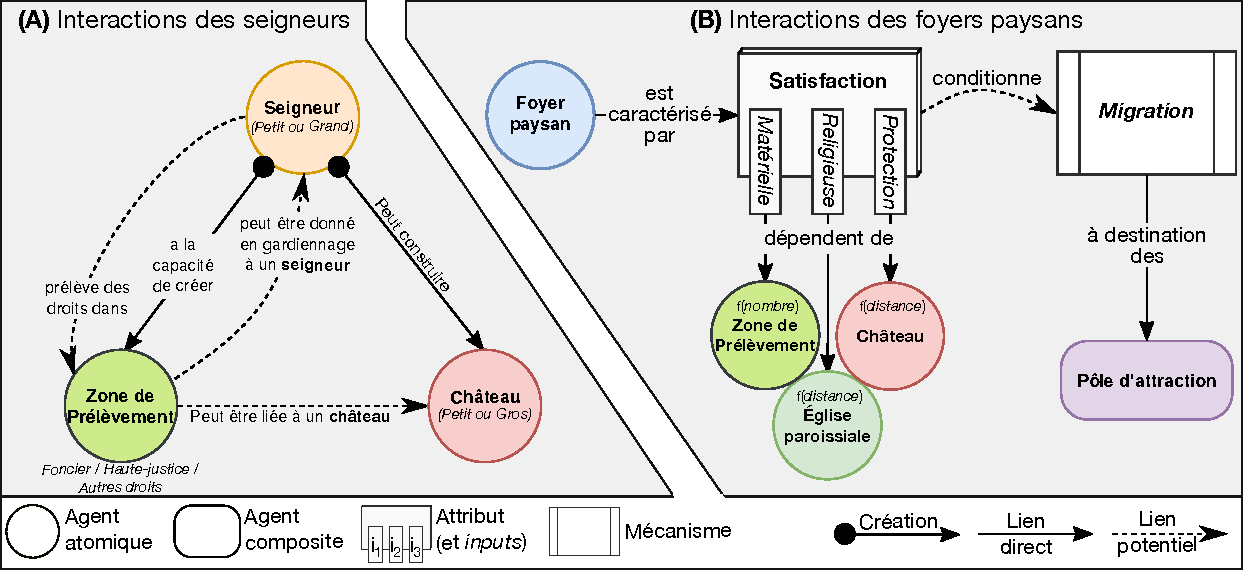
\includegraphics[width=\linewidth]{img/agents_interactions.pdf}
	\caption[Interactions des agents : seigneurs et foyers paysans.]{Interactions des agents : seigneurs (\textbf{A}) et foyers paysans (\textbf{B}).}
	\label{fig:interactions-agents}
\end{figure}

\medskip

Les agents pouvant influencer le niveau de satisfaction ou d'insatisfaction des foyers paysans peuvent être catégorisés en cinq groupes, en fonction de la nature de leur relation avec les foyers paysans.
Les trois premiers sont liés à leur niveau de satisfaction, les deux derniers influent directement sur leur comportement migratoire :
\begin{itemize}
	\item Les agents \og \textbf{seigneurs}\fg{} et les agents \og \textbf{zones de prélèvement}\fg{} : \\
	un foyer paysan doit s'acquitter de droits qui sont \ul{prélevés} par des seigneurs au sein de zones de prélèvement qu'ils \ul{créent}.
	Ces zones sont une représentation spatiale des droits dont les agents-seigneurs disposent sur les agents-foyers paysans :
		\textit{droits fonciers}, \textit{droits de haute justice} et \textit{autres droits} (droits banaux, droits de basse justice, etc.) (\cref{fig:interactions-agents}-\textbf{A}).
	En prélevant des droits, les seigneurs gagnent de la \textit{puissance} et, à l'inverse, l'importance des droits prélevés influe sur l'insatisfaction matérielle des foyers paysans.
	
	\item Les agents \og \textbf{églises}\fg{} et \og \textbf{paroisses}\fg{} : \\
	les agents \og églises\fg{} offrent aux foyers paysans les services religieux dont ils ont besoin.
	Certaines de ces églises ont acquis des \textit{droits paroissiaux}, et ont le statut d'églises paroissiales, ce qui constitue une \ul{promotion} (voir \cref{fig:constitution-agents}).
	La satisfaction religieuse des foyers paysans dépend de la distance à l'église paroissiale la plus proche (\cref{fig:interactions-agents}-\textbf{B}).
	Le territoire est maillé par des agents-paroisses, qui constituent le pendant surfacique des églises paroissiales (ponctuelles) et visent à desservir la population (\cref{fig:constitution-poles-paroisses}-\textbf{B}).
	
	\item Les agents \og \textbf{châteaux}\fg{} qui ont la capacité de protéger les foyers paysans face aux violences de l'époque (guerres, pillages, bandits, etc.).
	La satisfaction relative à cette protection est mesurée en fonction de la distance au château le plus proche.
	Ces châteaux sont \ul{construits} par les seigneurs tout au long de la simulation, en fonction de leur puissance.
	
	\item Les agents \og \textbf{agrégats} de foyers paysans\fg{} : \\
	ces agrégats sont des agents \og composites\fg{}\footnote{
	Par opposition aux autres types d'agents, dénommés \og atomiques\fg{} dans la \cref{fig:interactions-agents}.
	} composés d'un ensemble suffisant (5) de foyers paysans situés à proximité les uns des autres (\cref{fig:constitution-agents}).
	Les agrégats sont des agents en tant que tel, composite puisque constitués par des foyers paysans, mais dotés de leurs propres attributs, telle que l'existence en leur sein d'une éventuelle \textit{communauté paysanne}.
	L'agrégat n'a pas de pérennité propre : il émerge quand les migrations des foyers paysans débouchent sur des regroupements dans l'espace.
	Si les foyers paysans qui le composent migrent ailleurs à un des pas de temps suivants, l'agrégat disparaît.
	
	\item Les agents \og \textbf{pôles d'attraction}\fg{} : \\
	il s'agit ici encore d'agents composites, cette fois constitués d'un ou de plusieurs \textbf{attracteurs}, c'est-à-dire des églises paroissiales, des châteaux ou des agrégats de foyers paysans (\cref{fig:constitution-poles-paroisses}-\textbf{A}).
	C'est vers un tel pôle que se dirige le foyer paysan qui a pris la décision de migrer (\cref{fig:interactions-agents}-\textbf{B}).
\end{itemize}

Le \cref{tab:agents-simfeodal} résume les propriétés et caractéristiques des différents agents de \simfeodal{}.

	\begin{figure}[H]
	\centering
	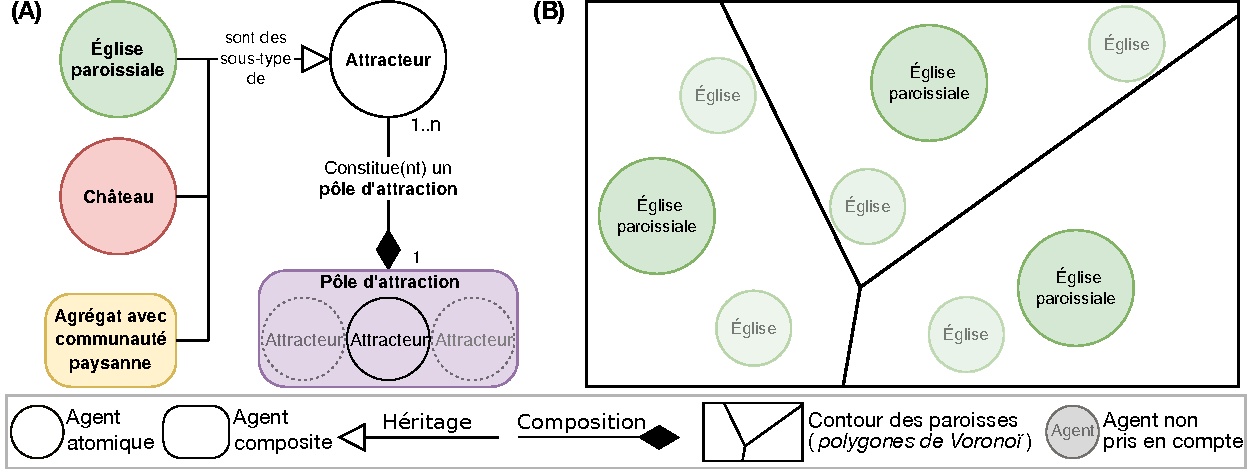
\includegraphics[width=\linewidth]{img/agents_paroisses_poles.pdf}
	\caption[Constitution des pôles d'attraction et des paroisses.]{Constitution des pôles d'attraction (\textbf{A}) et des paroisses (\textbf{B}).\\
		\textit{Exemple de lecture : un pôle d'attraction est composé de 1 ou plusieurs attracteurs ;
			un attracteur peut être une église paroissiale, un château ou un agrégat contenant une communauté paysanne ;
			un pôle d'attraction est ainsi composé d'un ou plusieurs de ces agents.}}
	\label{fig:constitution-poles-paroisses}
\end{figure}




\begin{figure}[H]
	\centering
	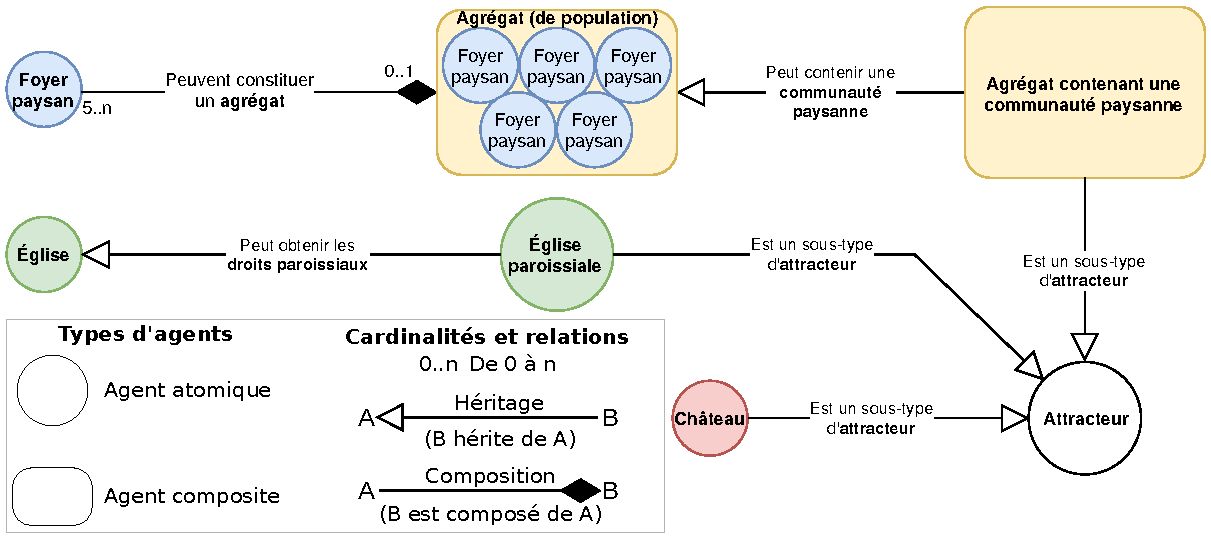
\includegraphics[width=\linewidth]{img/agents_constitution.pdf}
	\caption[Héritages et compositions des agents de \simfeodal{}.]{Héritages et compositions des agents de \simfeodal{}.\\
		\textit{Exemple de lecture :\\
			- un agrégat est composé de 5 ou plus foyers paysans,\\
			- un foyer paysan appartient à 0 ou 1 agrégat.}}
	\label{fig:constitution-agents}
\end{figure}

%Ces agents mobiles répondent à des mécanismes d'agrégation et de migration en fonction de leurs niveaux de \textit{satisfactions}, sur les plans matériel, spirituel et en terme de protection face aux violences.
%Les satisfactions sont mesurées respectivement en fonction des droits prélevés par des \textbf{Seigneurs} au sein de \textbf{Zones de Prélèvements} (satisfaction matérielle) ; en fonction de leur distance aux \textbf{églises paroissiales} les plus proches (satisfaction religieuse) ; et en fonction de leur distance aux \textbf{châteaux} -- construits par les \textbf{Seigneurs} -- les plus proches (satisfaction protection).
%Un niveau de satisfaction trop faible pousse les Foyers Paysans à migrer, soit dans un rayon local soit de manière globale.
%Lors de ces migrations, les Foyers Paysans sont attirés par des \textbf{Pôles}, ensembles composites d'\textbf{Attracteurs} (\textbf{châteaux}, \textbf{églises paroissiales} et \textbf{agrégats} de population) qui jouent un rôle de fixation de la population.
%Plus l'attractivité de ces pôles est importante, plus grandes sont leur chance d'attirer suffisamment de Foyers Paysans pour que ces derniers forment des \textbf{Agrégats} de population.
%Cela leur apportera alors un surcroît de satisfaction et permettront de fixer les Foyers Paysans présents et d'en attirer de nouveaux pour faire émerger une hiérarchie dans le système de peuplement.
%Le \cref{tab:agents-simfeodal} résume les propriétés et caractéristiques de ces différents types d'agents.

\begin{table}[H]
	\centering
	\footnotesize
	{\renewcommand{\arraystretch}{1}%
	\setlength\arrayrulewidth{1pt}\arrayrulecolor{black}
	\begin{tabular}{|M{1.75cm}|M{1.75cm}|M{2cm}|M{2cm}|M{4cm}|}
		\hline
		\textbf{Agent} & \textbf{Sous-type} & \makecell{\textbf{Quantité}\\ \textit{\small{(en 1200)}}} & \textbf{Emprise spatiale$^\upalpha$} & \textbf{Comportements actifs$^\upbeta$} \\ \hline
		
		\rowcolor[HTML]{dae8fc} \multicolumn{2}{|c|}{Foyers Paysans} & \makecell{$\approx$ 4 000 à \\75 000} & Ponctuelle & Migrations \\ \hline
		
		\rowcolor[HTML]{ffe6cc} Seigneurs & \makecell{Grands\\Seigneurs} & $\approx$ 2 & --- & \makecell{Création de zones de\\prélèvement,} \\ \hhline{|>{\arrayrulecolor[HTML]{ffe6cc}}->{\arrayrulecolor{black}}--->{\arrayrulecolor[HTML]{ffe6cc}}-}
		\rowcolor[HTML]{ffe6cc} & \makecell{Petits\\Seigneurs} & $\approx$ 200 & Ponctuelle & \makecell{collecte de droits,\\ construction de châteaux} \\ \hhline{|>{\arrayrulecolor{black}}-----}
		
		\rowcolor[HTML]{cdeb8b} & Foncier & $\approx$ 75 &  &  \\ \hhline{|>{\arrayrulecolor[HTML]{cdeb8b}}->{\arrayrulecolor{black}}-->{\arrayrulecolor[HTML]{cdeb8b}}--}
		\rowcolor[HTML]{cdeb8b} \makecell{Zones de\\ Prélèvement} & Haute-Justice & $\approx$ 50 & Zonale & --- \\ \hhline{|>{\arrayrulecolor[HTML]{cdeb8b}}->{\arrayrulecolor{black}}-->{\arrayrulecolor[HTML]{cdeb8b}}--}
		\rowcolor[HTML]{cdeb8b} & Autres droits & $\approx$ 300 &  &  \\ \hhline{|>{\arrayrulecolor{black}}-----}
		
		\rowcolor[HTML]{d5e8d4} {Églises} & Églises & $\approx$ 300 & {Ponctuelle} & --- \\ \hhline{|>{\arrayrulecolor[HTML]{d5e8d4}}->{\arrayrulecolor{black}}-->{\arrayrulecolor[HTML]{d5e8d4}}->{\arrayrulecolor{black}}-}
		\rowcolor[HTML]{d5e8d4} & Églises paroissiales$^\upgamma$ & $\approx$ 200 &  & \makecell{Création de paroisse} \\ \hhline{|>{\arrayrulecolor{black}}-----}
		
		\rowcolor[HTML]{d5e8d4} \multicolumn{2}{|c|}{\cellcolor[HTML]{d5e8d4} Paroisses} & $\approx$ 200 & Zonale & --- \\ \hhline{|>{\arrayrulecolor{black}}-----}
		
		\rowcolor[HTML]{f8cecc} \multirow{2}{*}{Châteaux$^\upgamma$} & Petits Châteaux & $\approx$ 40 & \multirow{2}{*}{Ponctuelle} &
		 \multirow{2}{*}{---} \\ \hhline{|>{\arrayrulecolor[HTML]{f8cecc}}->{\arrayrulecolor{black}}-->{\arrayrulecolor[HTML]{f8cecc}}--}
		\rowcolor[HTML]{f8cecc} & Gros Châteaux & $\approx$ 10 &  & \\ \hhline{|>{\arrayrulecolor{black}}-----}
		
		\rowcolor[HTML]{fff2cc} \multicolumn{2}{|c|}{Agrégats de population$^\upgamma$} & $\approx$ 200 & Zonale & \makecell{Création de communautés} \\ \hhline{|>{\arrayrulecolor{black}}-----}
		
		\rowcolor[HTML]{e1d5e7} \multicolumn{2}{|c|}{Pôles d'attraction} & $\approx$ 300 & Zonale & \makecell{Attire les Foyers Paysans} \\ \hhline{|>{\arrayrulecolor{black}}-----}
		\end{tabular}}
		\caption[Les différents types d'agents de SimFeodal.]{Les différents types d'agents de SimFeodal.\\
	\textit{$\upalpha$ : Les agents sans emprise spatiale (---) ne sont pas localisés dans l'espace du modèle.\\
		$\upbeta$ : Les agents sans comportements actifs (---) n'agissent pas en tant que tel, mais peuvent servir de support pour les actions d'autres agents.\\
		$\upgamma$ : Ces agents sont également des types d'attracteurs, qui constituent des pôles d'attraction, voir \cref{fig:constitution-poles-paroisses}-\textbf{A}.}}
		\label{tab:agents-simfeodal}
		\end{table}
\clearpage
\subsection{Échelles spatiales et temporelles}

\subsubsection{Résolution et échelle spatiale \label{subsec:reso-spatiale}}

L'espace du modèle est un monde théorique \textbf{isotrope}, \textbf{continu}, symbolisé sous la forme d'un \textbf{carré de 80 km de côté}, strictement \textbf{endogène} au modèle, c'est-à-dire créé (et recréé) à chaque nouvelle simulation.

\paragraph[Isotrope]{} Le monde est \textbf{isotrope} car il ne présente aucune hétérogénéité de surface ou de topologie.
La distance entre deux points est mesurée de manière euclidienne.
Cet espace support se veut le plus neutre et simple possible.
Il est ainsi susceptible de représenter un cas très général, qui peut servir de support à toute la diversité des espaces de l'Europe du Nord-Ouest, par l'entremise de ce dessin théorique.

\paragraph[Continu]{}Contrairement à ce qui se fait usuellement en simulation à base d'agents, nous avons aussi fait le choix de placer \simfeodal{} dans \textbf{un espace continu}, c'est-à-dire non discrétisé.
La discrétisation de l'espace, sous forme de \og patchs\fg{} ou de \og cellules\fg{}, s'inscrit souvent dans l'héritage des modèles à base d'automates cellulaires.
Les \textit{patchs} prennent d'ordinaire la forme d'agents : cela facilite l'attribution de caractéristiques, comme un certain niveau de ressource, une altitude, une population agrégée etc.
Dans le cas de \simfeodal{}, l'espace n'est qu'un support: il ne possède aucune caractéristique propre.
Par sa nature isotropique, il n'est pas utile d'y différencier d'éventuelles cellules les unes des autres.
Une large part des mécanismes de \simfeodal{} s'appuie sur la prise en compte de distances entre agents, à partir de seuils dont les ordres de grandeur peuvent être très variables (de la centaine de mètres à plus de 10 km).
Nous avons préféré ne pas procéder à une discrétisation de l'espace, compte tenu de cette variabilité, afin de ne pas artificiellement réduire la précision des relations spatiales.


\paragraph[Dimension]{}L'espace est formalisé sous la forme d'\textbf{un carré de 80 km de côté}, proche de l'ordre de grandeur des diocèses médiévaux, maillage territorial relativement stable dans le temps depuis cette époque médiévale jusqu'à aujourd'hui.
Dans des versions précédentes de \simfeodal{}, le carré avait un côté de 100 km. Nous avons choisi de le réduire afin d'approcher de la superficie de la Touraine médiévale sur laquelle nous prenons appui pour le calibrage du modèle. 
La superficie du département d'Indre-et-Loire actuel, ou encore du diocèse de Tours qui est à peu près équivalent à ce département, sont d'environ 6 000 km².
En choisissant un espace support de 80 $\times$ 80 km (6 400 km²), on facilite l'estimation des densités et mesures d'écartements dans le modèle au regard des connaissances empiriques.
Notons enfin que si l'espace support est bien un carré de 80 km de côté, on en retranche en réalité une partie (1 km de chaque côté, voir \cref{fig:espace-simfeodal}) pour définir un espace utile, ou \og espace actif\fg{}.
On s'assure ainsi qu'aucune localisation ne soit située trop proche des limites de l'espace, ce qui pourrait avoir pour effet de produire des \og effets de bords\fg{}, aussi bien informatiques qu'en termes d'anomalies de voisinages.
L'espace actif, utilisable dans le modèle, est donc de 79 $\times$ 79 km, soit 6 084 km².

\begin{figure}[H]
	\centering
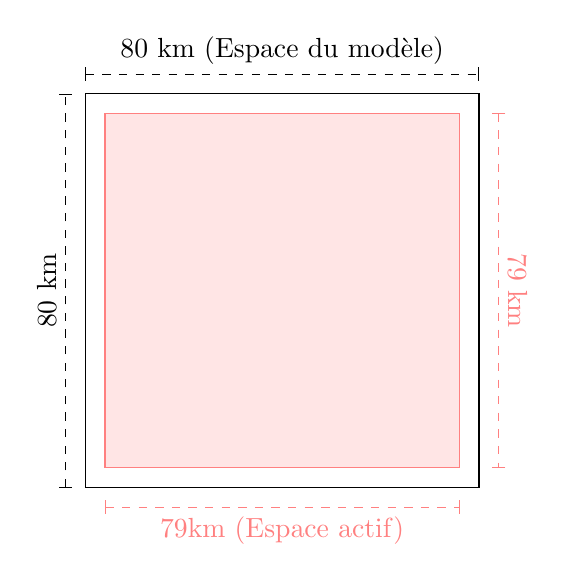
\begin{tikzpicture}[scale=.5]
\draw[] (0,0) -- (0,10) -- (10,10) -- (10,0) -- cycle;
\draw[|-|, very thin, dashed] (0, 10.5) -- node[above] {80 km (Espace du modèle)} (10, 10.5);
\draw[|-|, very thin, dashed] (-0.5, 0) -- node[above, rotate=90] {80 km} (-0.5, 10);

\draw[color=red!50, fill = red!10] (0.5, 0.5) -- (0.5, 9.5) -- (9.5, 9.5) -- (9.5, 0.5) -- cycle;
\draw[|-|, very thin, dashed, red!50] (10.50, 9.50) -- node[above, red!50, rotate=-90] {79 km} (10.5, 0.5);
\draw[|-|, very thin, dashed, red!50] (0.5, -0.5) -- node[below, red!50] {79km (Espace actif)} (9.5, -0.5);
\end{tikzpicture}
\caption[L'espace support de SimFeodal, un monde théorique.]{L'espace support de SimFeodal, un monde théorique.\\
\textit{N.B : Dans le schéma, pour une question de lisibilité, les dimensions de l'espace réduit ne sont pas proportionnelles à celles de l'espace d'ensemble.}}
\label{fig:espace-simfeodal}
\end{figure}

\paragraph[Endogène]{} Notons enfin que l'espace est strictement \textbf{endogène} au modèle.
On entend par là que le monde simulé ne résulte pas d'un \textit{input}\footnote{
	Contrairement à de nombreux modèles utilisés en géographie \autocites[etc.]{white_use_1997,white_high-resolution_2000,dubos-paillard_analyse_2003,benenson_schelling_2009}, il n'y a pas de chargement de configurations initiales dans \simfeodal{} : la génération de l'espace support est un sous-modèle dans le modèle.
} : seul un paramètre, qui régit la taille des côtés, joue sur la géométrie globale de l'espace.
%Il nous semble important de le préciser, en particulier parce que c'est, à notre connaissance, assez inhabituel dans la simulation de données géographiques, mêmes théoriques.
Les agents sont en effet placés, à l'échelle de l'individu, de manière quasi-aléatoire dans l'espace du modèle.
Cet aléa est toutefois contrôlé à l'échelle du système: la structure d'ensemble du peuplement répond à des caractéristiques choisies et paramétrées.
Cette localisation des agents doit répondre à une double contrainte:
\begin{itemize}
	\item Au niveau des agents, la distribution spatiale doit être aléatoire, afin que les différentes situations spatiales générées présentent une large diversité.
	Cette diversité, éprouvée par l'exécution de nombreuses réplications du modèle, est garante de la généricité du modèle.
	\item Au niveau global, la structure du système de peuplement généré doit être partiellement configurable, c'est-à-dire répondre à certains paramètres macroscopiques qui agiront sur le degré de concentration ou de dispersion dans l'ensemble de l'espace \og actif\fg{} des foyers paysans.
\end{itemize}


\subsubsection{Granularité temporelle}

\simfeodal{} modélise des processus qui se déroulent sur le temps long, et à ce titre, la gestion de la temporalité est importante.
Le modèle inscrit son exécution dans une étendue de \textbf{400 ans}, \textbf{discrétisée} sous la forme de 20 pas de temps de \textbf{20 ans} chacun.

\paragraph[Durée]{} La période d'étude, thématique, s'étend entre 800 après J.-C. et 1100, qui correspondent à des repères temporels entre lesquels on estime que la transition s'est déroulée (\cref{subsec:contexte-historio}).
Pour modéliser ces évolutions, nous avons choisi de commencer à la même date, mais de prolonger l'exécution du modèle d'un siècle, soit de \textbf{de 800 à 1200}\footnote{
	Dans les versions précédentes de \simfeodal{} (par exemple dans \textcite{cura_transition_2017}), cette date était fixée à 1160.
	Nous avons choisi de prolonger de 40 ans la date de fin parce que cela 
	permet de comparer l'état final du modèle au début du XIII$^e$ siècle, pour lequel certaines données empiriques supplémentaires sont disponibles.
	On obtient de plus un nombre de pas de temps plus \og rond\fg{} (20) qu'auparavant (18), ce qui permet par exemple de représenter l'évolution d'une simulation de manière plus régulière.
}.
Prolonger cette date d'observation des résultats du modèle permet d'analyser le comportement du modèle après la période même de la transition identifiée, à une date où le système de peuplement est pleinement inscrit dans son régime post-transition (régime 2, cf. \cref{subsec:processus-longue-duree}).
On peut ainsi, entre autres, voir si les processus à l'œuvre subissent bien un ralentissement, marquant par exemple la fin de la féodalité, plutôt qu'un accroissement constant.

\paragraph[Discret]{} Contrairement à la gestion de l'espace, nous avons choisi de modéliser le temps sous forme \textbf{discrète}.
Ce choix s'explique par deux raisons principales.
En premier lieu, la transition s'inscrit dans une forte incertitude temporelle. 
Les experts thématiciens peuvent certes s'appuyer sur des dates précises, par exemple pour des années de réformes, mais les processus à l'œuvre s'inscrivent dans une durée difficile à préciser.
Le niveau de résolution temporel de ces processus est difficilement réductible à moins d'un demi-siècle, et à peine meilleur pour les éléments matériels.
Une vision continue du temps s'inscrirait ainsi dans une certaine sur-détermination du modèle par rapport aux connaissances thématiques sur lesquelles il s'appuie.
En second lieu, les processus sont modélisés à un niveau de résolution correspondant à celui des \og foyers paysans\fg{}, c'est-à-dire à l'échelle de foyers plus que d'individus.
Les migrations des foyers paysans correspondent empiriquement plutôt à des déplacements qui surviennent à l'échelle temporelle de la génération.
Cela signifie que ces migrations se réalisent en fait quand les descendants d'un foyer sont en âge de s'établir dans une nouvelle localisation.
La prise en compte d'un temps continu impliquerait la mise en place de bien plus de mécanismes probabilistes, avec des aberrations potentielles plus importantes en termes de trajectoires des agents.

\paragraph[Pas de temps de 20 ans]{} L'inscription thématique du mécanisme de migration oriente le choix de la granularité du modèle.
\textbf{Les pas de temps ont une durée de 20 ans}, ce qui correspond à peu près à la durée d'une génération à l'époque, c'est-à-dire à l'âge auquel les individus sont en mesure de se marier et de fonder un noyau familial différent de celui de leurs ascendants.
Cela correspond aussi à la précision globale que l'on peut avoir de l'apparition d'éléments matériels tels que les églises, paroisses et châteaux\footnote{
	Certains de ces éléments sont connus avec une précision bien supérieure, par exemple quand des textes historiques mentionnent leur création.
	Ce n'est toutefois pas généralisé, et la précision moyenne est généralement de l'ordre de 20 à 40 ans.
}.
Dans l'ensemble, au vu des connaissances historiques, ces pas de temps doivent être interprétés comme des repères temporels plus que comme des dates précises. 
Que les premiers châteaux apparaissent en 980 ou en 1000 n'a pas d'importance dans le modèle, tant que cela se déroule avant le milieu du XI$^e$ siècle par exemple.

La \cref{fig:frise-chrono} illustre les processus et événements qui surviennent pendant l'ensemble de cette période.
Elle donne à voir la correspondance floue entre les événements historiques, précis ou non, et leur implémentation dans \simfeodal{}.
Cette dernière peut ainsi prendre la forme de changements datés (par exemple le début du mécanisme de don de châteaux), ou au contraire de mises en place graduelles de mécanismes (par exemple les gains de droits de haute justice par les grands seigneurs, qui sont progressifs).

\begin{figure}[H]
	\centering
	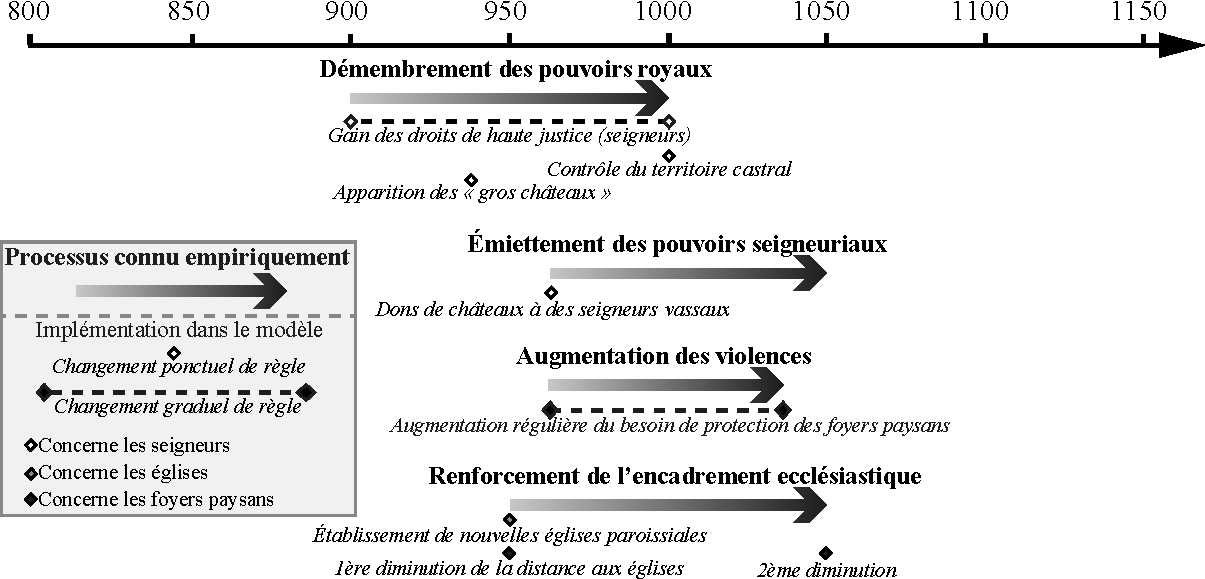
\includegraphics[width=\linewidth]{img/frise_chrono_tmd.pdf}
	\caption[Frise chronologique des processus historiques observés en Touraine implémentés dans \simfeodal{}.]{Frise chronologique des processus historiques observés en Touraine implémentés dans \simfeodal{}. D'après \textcite[fig. 2, p.~315]{cura_transition_2017}.}
	\label{fig:frise-chrono}
\end{figure}



\let\orisectionmark\sectionmark
\renewcommand\sectionmark[1]{}%
\section[Fonctionnement général -- \textit{Process overview and schedulling}]{Fonctionnement général -- \large{\textit{Process overview and schedulling}}\label{sec:fonctionnement-general}}
\orisectionmark{Fonctionnement général}
\let\sectionmark\orisectionmark

\simfeodal{} est un modèle qui s'inscrit plutôt dans une approche KIDS que KISS (voir \cref{chap:chap1}, \cref{subsec:explorer-confronter}).
Il est constitué d'une large variété d'agents (\cref{tab:agents-simfeodal}) dotés, pour certains, de nombreux comportements.
Au total, ce sont près de quarante mécanismes particuliers (ici regroupés en une quinzaine de mécanismes généraux) qui font interagir les agents à chaque pas de temps.
Dans cette partie, nous présentons une synthèse de ces mécanismes, sans entrer dans le détail, algorithmique ou mathématique, de chacun, en accord avec les spécifications du formalisme ODD (voir la \cref{sec:meca-specifiques} pour des descriptions plus précises des mécanismes les plus complexes et importants).
Par ailleurs, afin de bien distinguer ce qui relève du domaine empirique, lié aux connaissances thématiques qui y sont associées, et ce qui relève du domaine du modèle et des choix de modélisation qui y sont opérés, les descriptions et commentaires associés à chacun de ces domaines apparaissent de manière différenciée dans le texte.
Les premiers sont présentés dans un format classique, tandis que les seconds sont encadrés en grisé.

Notons enfin que dans le cas des \og mécanismes globaux\fg{}\footnote{
	C'est-à-dire les mécanismes ne correspondant pas à des \og réflexes\fg{} ou actions des agents, mais qui servent à modifier l'état \og global\fg{} du modèle.
	Par exemple, l'initialisation du monde simulé est un processus global : ce n'est pas un agent qui, par son comportement, va créer le monde simulé, mais un mécanisme global qui suit une logique procédurale programmée par le modélisateur.
} et de certains mécanismes très techniques (mise à jour des agrégats ou des pôles par exemple), la description des mécanismes ne s'appuiera pas sur une description empirique : ce sont des contraintes et choix propres à la description du monde -- et de ses caractéristiques spatiales -- dans lequel les agents qui sont présentés interagissent.
Certains de ces mécanismes peuvent être guidés par les connaissances expertes, mais ils peuvent aussi remplir un rôle purement technique (enregistrement des \textit{outputs} par exemple), nécessaire au bon fonctionnement du modèle mais n'ayant pas d'inscription ou de correspondance empirique.

\subsection*{Ordonnancement général \label{meca-ordonancement}}

\begin{figure}[H]
	\centering
	% Couleurs
	\definecolor{col-fp}{HTML}{dae8fc}
	\definecolor{col-agregats}{HTML}{fff2cc}
	\definecolor{col-seigneurs}{HTML}{ffe6cc}
	\definecolor{col-eglises}{HTML}{d5e8d4}
	\definecolor{col-poles}{HTML}{e1d5e7}
	\definecolor{col-global}{HTML}{F5F5F5}
	% Styles des noeuds et lignes
	\tikzstyle{block} = [rectangle, draw, minimum width=4em, align=center, rounded corners, minimum height=2em, thick]
	\tikzstyle{start} = [draw, circle, minimum height=2em, align=center, thick]
	\tikzstyle{temp} = [very thick, dashed]
	\tikzstyle{line} = [draw, -{Latex[length=2.5mm,width=2.5mm]}]
	\tikzstyle{dline} = [draw, -{Latex[length=2.5mm,width=2.5mm,black!50]}, black!50, densely dotted]
	% 
	\tikzstyle{fps} = [fill=col-fp]
	\tikzstyle{agregats} = [fill=col-agregats]
	\tikzstyle{poles} = [fill=col-poles]
	\tikzstyle{seigneurs} = [fill=col-seigneurs]
	\tikzstyle{globals} = [fill=col-global]
	\tikzstyle{eglises} = [fill=col-eglises]

	\begin{tikzpicture}[node distance = .75cm and .75cm, auto, scale=0.7,every node/.style={transform shape}]
	% Place nodes
	\node [start, globals] (init) at (0,0) {Init.\\du\\monde};
	
	\node [start ,right= of init] (start) {Début\\du tour};
	\node [block, globals,right= of start] (maj-globals) {MaJ* des \\variables\\globales};
	\node [block, fps, right= of maj-globals] (renouvellement-fp) {Renouvellement\\des FP**};
	\node [block, eglises,right= of renouvellement-fp] (maj-paroisses) {Détection et\\promotions des\\paroisses};
	\node [block, poles, right = of maj-paroisses] (maj-poles) {Détection\\des\\Pôles};
	
	\node [block, fps, below= of maj-poles] (maj-satisfaction) {MaJ* satisfactions des FP**};
	\node [block, fps, below=of maj-satisfaction] (migration-fp) {Migration des FP**};
	\node [block, seigneurs, temp, below =of migration-fp] (maj-droits) {Gains de \\droits des seigneurs};
	\node [block, seigneurs, below=of maj-droits] (maj-zp) {Collecte des droits};
	
	\node [block, seigneurs, left=of maj-zp] (maj-dons) {Dons droits\\ et châteaux\\des Seigneurs};
	\node [block, seigneurs, temp, left=of maj-dons] (promo-chateaux) {Promotion\\des châteaux};
	\node [block, seigneurs, temp, left=of promo-chateaux] (constructions-chateaux) {Construction\\ de châteaux};
	\node [block, seigneurs, left=of constructions-chateaux] (creation-seigneurs) {Création des\\nouveaux Seigneurs};		
	
	\node [block, agregats, above= of creation-seigneurs] (maj-agregats) {MaJ* des Agrégats};
	\node [block, poles, above=of maj-agregats] (maj-poles2) {MaJ* des Pôles};
	\node [block, globals, above= of maj-poles2] (maj-outputs) {MaJ* et enregistrement\\des \textit{outputs}};

	
	\path[line]%
	(maj-globals) -- (renouvellement-fp)
	(renouvellement-fp) -- (maj-paroisses)
	(maj-paroisses) -- (maj-poles)
	(maj-poles) -- (maj-satisfaction)
	(maj-satisfaction) -- (migration-fp)
	(migration-fp) -- (maj-droits)
	(maj-droits) -- (maj-zp)
	(maj-zp) -- (maj-dons)
	(maj-dons) -- (promo-chateaux)
	(promo-chateaux) -- (constructions-chateaux)
	(constructions-chateaux) -- (creation-seigneurs)
	(creation-seigneurs) -- (maj-agregats)
	(maj-agregats) -- (maj-poles2)
	(maj-poles2) -- (maj-outputs);

	
	\path[line] (init)-- (start);
	\path[line] (start) -- (maj-globals);
	\path[dline] (maj-outputs)-- (start);	
	\end{tikzpicture}
	\caption[Ordonnancement des mécanismes de SimFeodal.]{Ordonnancement des mécanismes de SimFeodal.\\
	{\footnotesize
	\colorbox{col-global}{\strut Mécanisme global} \colorbox{col-fp}{\strut Foyers Paysans} \colorbox{col-eglises}{\strut Églises} \colorbox{col-agregats}{\strut Agrégats} \colorbox{col-poles}{\strut Pôles} \colorbox{col-seigneurs}{\strut Seigneurs} \dbox{\strut Temporaire}.\\
	{\strut MaJ* : \og Mise à jour\fg{}; FP** : \og Foyers paysans\fg{}}
	}
	}
	\label{fig:ordonnancement}
\end{figure}

\begin{tcolorbox}[breakable,left=0pt,right=0pt,top=0pt,bottom=0pt,
	colback=gray!15,colframe=gray!15,width=\dimexpr\textwidth\relax, 
	enlarge left by=0mm, boxsep=5pt,arc=0pt,outer arc=0pt]
	
Dans \simfeodal{}, les mécanismes sont toujours appelés dans le même ordre (voir \cref{fig:ordonnancement}): l'ordonnancement ne change pas tout au long des 20 pas de temps du modèle.
Certains mécanismes sont toutefois temporaires, c'est-à-dire rendus inactifs en fonction des pas de temps: la construction des châteaux, par exemple, n'est pas possible avant 940.
Jusqu'au pas de temps correspondant, le mécanisme est alors désactivé par un paramètre réglable.
Notons que si les mécanismes suivent un ordre déterminé, ce n'est pas le cas des agents qui y sont associés.
Pour un mécanisme donné, l'ordre d'appel des agents est aléatoire et varie à chaque appel de ce mécanisme.
\end{tcolorbox}


\subsection{Initialisation \label{meca-init}}

L'étape d'initialisation du \og monde\fg{} simulé consiste à créer l'espace théorique dans lequel les agents vont interagir, et à générer ces derniers.
Il s'agit ainsi de créer et de localiser les églises, paroissiales ou non, les seigneurs, et surtout, les foyers paysans.
Ces derniers, empiriquement, sont majoritairement dispersés dans la région d'étude, mais aussi regroupés localement, au sein de villages et d'agglomérations secondaires antiques.

\begin{tcolorbox}[breakable,left=0pt,right=0pt,top=0pt,bottom=0pt,
	colback=gray!15,colframe=gray!15,width=\dimexpr\textwidth\relax, 
	enlarge left by=0mm, boxsep=5pt,arc=0pt,outer arc=0pt]
Pendant cette étape, des foyers paysans sont générés et localisés dans l'espace du modèle.
Comme indiqué dans la \cref{subsec:reso-spatiale}, cette localisation des foyers paysans doit répondre à une double contrainte : aléatoire localement, mais organisée selon une structure macrogéographique prédéfinie.
Pour que ces deux contraintes, d'apparence contradictoires, soient respectées, les agents sont très majoritairement localisés de manière aléatoire, mais certains sont répartis \og par groupe\fg{} dans le monde simulé.
La localisation de ces groupes est aléatoire, mais leurs propriétés (nombre de foyers paysans par exemple) dépendent de paramètres du modèle (voir \cref{sec:initialisation}).

\medskip
Quelques dizaines d'agents sont ainsi localisés de manière agrégée afin de constituer les premiers agrégats de population, de tailles variables (une vingtaine de villages peu peuplés, et quelques petites villes plus importantes qui correspondent aux agglomérations secondaires antiques).
Lors de l'initialisation sont aussi créés les premiers seigneurs -- grands seigneurs sans portée spatiale et petits seigneurs localisés aléatoirement dans l'espace -- et les zones de prélèvement dans lesquelles ils prélèveront des droits divers.
Ces zones de prélèvement sont matérialisées sous formes de cercles de rayons variables, dont le centre correspond à la localisation des seigneurs qui les créent.
Dès le départ de la simulation, l'espace support constitue ainsi une contrainte pour les foyers paysans qui se verront prélever des droits dans ces zones.

L'initialisation est enfin l'occasion de créer et de disperser dans l'espace des églises (150).
Parmi celles-ci, quelques-unes (50), choisies aléatoirement, se verront dotées de droits paroissiaux.
Ces églises paroissiales constitueront ainsi le semis autour duquel sera organisé le premier maillage paroissial.
\end{tcolorbox}

\subsection{Variables globales \label{meca-variables}}


\begin{tcolorbox}[breakable,left=0pt,right=0pt,top=0pt,bottom=0pt,
	colback=gray!15,colframe=gray!15,width=\dimexpr\textwidth\relax, 
	enlarge left by=0mm, boxsep=5pt,arc=0pt,outer arc=0pt]
Plusieurs mécanismes de \simfeodal{} évoluent au cours du temps, c'est-à-dire qu'ils changent de mode de fonctionnement d'une période à l'autre.
Telle est la possibilité, évoquée plus haut, pour les seigneurs de construire un château, mais aussi, l'évolution des distances que les foyers paysans sont prêts à parcourir pour se rendre à l'église, etc.
La mise en place de mécanismes tributaires de dates nous permet ainsi de représenter des événements exogènes au modèle, qui peuvent dès lors servir de déclencheurs ou de catalyseurs à des processus de longue durée.
L'incrémentation de la date et les mises à jour des différentes variables temporelles constituent donc la première étape de chaque nouvelle itération du modèle.
\end{tcolorbox}

\subsection{Renouvellement des foyers paysans \label{meca-renouvellement}}

\simfeodal{} est un modèle qui simule l'évolution d'un système spatial clos.
On entend par là qu'il n'y a pas d'échange ou d'interaction avec les régions voisines, situées hors du carré qui tient lieu de monde simulé.
C'est une limite forte, par ailleurs fréquente dans la modélisation où l'espace joue un rôle, car empiriquement, les systèmes sont rarement entièrement fermés et isolés.
Il est ainsi difficile de s'abstraire du contexte spatial, en particulier dans un modèle simulant des migrations.
Le monde modélisé constitue certes un système en lui-même, mais c'est aussi un système qui n'est qu'une des composantes d'un système de peuplement plus large (le royaume des Francs, voire l'Europe du Nord-Ouest anciennemnt romanisée).

\begin{tcolorbox}[breakable,left=0pt,right=0pt,top=0pt,bottom=0pt,
	colback=gray!15,colframe=gray!15,width=\dimexpr\textwidth\relax, 
	enlarge left by=0mm, boxsep=5pt,arc=0pt,outer arc=0pt]
Nous avons choisi de modéliser les échanges avec l'extérieur par le biais d'un renouvellement partiel des foyers paysans.
À chaque pas de temps, une part (5\%) des foyers paysans existant est supprimée de la simulation, et une quantité équivalente est réinjectée dans l'espace du modèle.
Afin de ne pas bouleverser de manière artificielle le processus émergent de concentration, la localisation dans l'espace des nouveaux foyers suit la proportion de foyers paysans dispersés et agrégés existants à la date considérée :
s'il y avait 90\% de foyers paysans dispersés avant le renouvellent, 90\% des foyers paysans ré-injectés seront localisés aléatoirement dans l'espace du modèle.
Les 10\% restant seront placés dans les agrégats existant selon un tirage aléatoire pondéré : les agrégats les plus peuplés attireront potentiellement plus de ces nouveaux foyers paysans que les moins peuplés\footnotemark.

\end{tcolorbox}
\footnotetext{
	Cette logique d'attachement préférentiel (voir \cref{subsec:basic-principles}) permet de modéliser l'attractivité qu'exercerait un agrégat peuplé, potentiellement plus connu, sur des foyers paysans venant de régions voisines.
}

\subsection{Mise à jour du maillage paroissial \label{meca-paroisses}}

Le Moyen Âge voit apparaître un maillage territorial dense, continu dans l'espace, constitué autour d'églises dotées de droits paroissiaux : les paroisses, qui organisent l'ensemble de la vie spirituelle de la population.
Les archéologues ne s'accordent pas sur la date de leur apparition (avant la période étudiée), ni sur le moment où elles constituent un maillage complet (vraisemblablement pendant la période modélisée).
Ils s'accordent cependant sur le rôle de fixation du peuplement et de stabilisation du territoire qu'elles ont eu \autocite{zadora-rio_paroisses_2008}.
On sait également, d'après les données et connaissances empiriques, que la répartition des églises paroissiales n'est pas homogène et qu'elle dessine des mailles de dimensions inégales.
Dans les zones rurales, l'espacement des églises paroissiales est assez important (quelques kilomètres entre deux églises), tandis que dans les zones urbaines, plusieurs églises paroissiales coexistent au sein d'une même ville.	

\begin{tcolorbox}[breakable,left=0pt,right=0pt,top=0pt,bottom=0pt,
	colback=gray!15,colframe=gray!15,width=\dimexpr\textwidth\relax, 
	enlarge left by=0mm, boxsep=5pt,arc=0pt,outer arc=0pt]
	Dans \simfeodal{}, le maillage paroissial est représenté par un diagramme de Voronoï autour des églises paroissiales.
	À chaque pas de temps, de nouvelles églises paroissiales apparaissent, à travers des mécanismes de promotion ou de création.
	Par construction, une tesselation de Voronoï dépend du semis de point à partir duquel elle est calculée.
	Il est donc nécessaire recalculer ce maillage à chaque fois que l'on ajoute ou supprime des points, en repartant d'une situation \og neutre\fg{} d'où l'on aura supprimé le maillage pré-existant\footnotemark.
	Le mécanisme de \og mise à jour\fg{} du maillage comprend donc plusieurs étapes de délimitation des paroisses (les mailles) et la création et promotion de nouvelles églises paroissiales.
\end{tcolorbox}
\footnotetext{
	Il n'y a pas pour autant de perte totale d'héritage : la tesselation de Voronoï est un processus déterministe, et si les églises paroissiales n'ont pas changé, le maillage sera identique.
	De plus, les répercussions des ajouts d'églises paroissiales sont assez localisées : si on ajoute une église paroissiale dans une zone déjà dense, par exemple dans un agrégat, les répercussions sur les mailles situées en dehors de cette zone seront minimes voire nulles.
}
	Le mécanisme de mise à jour du maillage paroissial s'effectue en trois étapes distinctes~:

\begin{itemize}
	\item \textbf{Dessin du maillage}
		\begin{tcolorbox}[breakable,left=0pt,right=0pt,top=0pt,bottom=0pt,
		colback=gray!15,colframe=gray!15,width=\dimexpr0.94\textwidth\relax, 
		enlarge left by=0mm, boxsep=5pt,arc=0pt,outer arc=0pt]
			Dans \simfeodal{}, le maillage paroissial est calculé et représenté sous la forme d'une partition de Voronoï autour des églises paroissiales.
			On garantit ainsi un pavage complet du territoire.
			Ce pavage sera lâche dans les zones les moins peuplées et dotées de 	moins d'églises paroissiales.
			Dans les zones les plus peuplées, telles que celles contenant les agrégats les plus importants, au contraire, il sera plus dense.
	\end{tcolorbox}
	
	\item \textbf{Création de paroisses \og urbaines\fg{}} Les agrégats de population sont localisés dans l'espace, et à ce titre, nécessairement inclus dans au moins une paroisse.
	Au fur et à mesure que les agrégats croissent, le nombre de foyers paysans que doit desservir chaque paroisse augmente.
	Empiriquement, on sait que plus le nombre de foyers paysans à desservir était important, plus forte était la probabilité de créer une nouvelle paroisse.
	
	\begin{tcolorbox}[breakable,left=0pt,right=0pt,top=0pt,bottom=0pt,
		colback=gray!15,colframe=gray!15,width=\dimexpr0.94\textwidth\relax, 
		enlarge left by=0mm, boxsep=5pt,arc=0pt,outer arc=0pt]
	\simfeodal{} comprend, pour modéliser cela, un mécanisme de création de paroisses.
	Selon une logique probabiliste, le modèle fait apparaître de nouvelles églises, directement dotées de droits paroissiaux, au sein des agrégats les plus peuplés.
	Plus un agrégat est peuplé, plus la probabilité est grande de voir apparaître, en son sein, une nouvelle église paroissiale dédiée à sa desserte.	
	Afin d'éviter l'apparition exponentielle d'églises paroissiales au sein d'un agrégat, cette probabilité est pondérée par le nombre d'églises paroissiales déjà présentes dans l'agrégat.
	La probabilité est donc fonction du nombre de foyers paysans par église paroissiale.
\end{tcolorbox}
	
	\item \textbf{Promotion de paroisses \og rurales\fg{}} Tout au long de son développement et à mesure de l'importance sociale qu'il acquiert, on sait que le maillage paroissial se densifie, pour parvenir en fin de période au maillage quasi-communal qui en est hérité aujourd'hui.
	Cette densification est observée partiellement dans les zones denses, mais aussi très largement et de manière homogène sur l'ensemble du territoire, notamment dans les zones les moins peuplées, afin de garantir un accès facilité aux sacrements à l'ensemble des foyers paysans.
	
	\begin{tcolorbox}[breakable,left=0pt,right=0pt,top=0pt,bottom=0pt,
		colback=gray!15,colframe=gray!15,width=\dimexpr0.94\textwidth\relax, 
		enlarge left by=0mm, boxsep=5pt,arc=0pt,outer arc=0pt]
	Dans le modèle \simfeodal{}, quand le nombre de foyers paysans de ces zones faiblement peuplé dépasse un seuil paramétré, de nouvelles églises paroissiales sont créées.
	Quand c'est possible, ces nouvelles églises paroissiales peuvent s'appuyer sur les églises locales existantes non dotées de droits paroissiaux.
	Quand il n'y a pas d'église non paroissiale à proximité, on construit de nouvelles églises qui deviendront centres paroissiaux.
	Les spécificités de ce mécanisme sont détaillées dans la section dédiée (\cref{sssec:paroisses}).
\end{tcolorbox}
\end{itemize}


%\paragraph{Dessin du maillage} Le maillage paroissial est calculé et représenté sous la forme d'une partition de Voronoï autour des églises paroissiales.
%On garantie ainsi un pavage complet du territoire.
%Ce pavage sera lâche dans les zones les moins peuplées et dotées de moins d'églises paroissiales.
%Dans les zones les plus peuplées, au contraire, il sera plus dense, comme par exemple dans les zones contenant les agrégats les plus importants.

%\paragraph{Création de paroisses \og urbaines\fg{}} Dans les agrégats les plus peuplés, certaines paroisses peuvent être amenées à regrouper des centaines de paroissiens, ce qui ne correspondrait pas aux connaissances empiriques.
%\simfeodal{} comprend donc un mécanisme de création de paroisses, via la construction d'églises dotées de droits paroissiaux, au sein des agrégats les plus peuplés, selon une logique probabiliste. 
%Plus un agrégat est peuplé, plus il a de probabilités de voir apparaître une nouvelle église paroissiale, dans son étendue, dédiée à sa desserte.
%
%Afin d'éviter l'apparition exponentielle d'églises paroissiales au sein d'un agrégat, cette probabilité est pondérée par le nombre d'églises paroissiales déjà présentes dans l'agrégat.
%Ainsi, là où un agrégat constitué de 1~000 foyers paysans et contenant une unique paroisse aura une probabilité de 50\% de voir apparaitre une nouvelle églises paroissiale, un agrégat constitué de 1~000 foyers paysans mais déjà doté de 2 paroisses n'aura qu'une probabilité de 25\%.

%\paragraph{Promotion de paroisses \og rurales\fg{}} Tout au long de son développement et à mesure de l'importance sociale qu'il acquière, on sait que le maillage paroissial se densifie, pour parvenir en fin de période au maillage quasi-communal qu'on lui connaît désormais.
%Cette densification est observée partiellement dans les zones denses, mais aussi très largement de manière homogène sur le territoire, notamment dans les zones les moins peuplées, afin de garantir un accès facilité aux sacrements à l'ensemble des foyers paysans.
%Dans ces zones, on fait apparaître de nouvelles églises paroissiales, soit par promotion d'églises existantes (non dotées de droits paroissiaux), soit par construction de nouvelles églises qui deviendront centres paroissiaux.
%Le mécanisme de ces créations est complexe, et on le détaille et l'illustre donc, à l'instar du détail des règles de création de paroisses \og urbaines\fg{}, dans la partie du chapitre relative aux spécificités des mécanismes (\cref{sssec:paroisses}).
%Notons simplement que là encore, la promotion ou création d'églises paroissiales en zones peu denses suit une logique de seuil : si une paroisse contient trop de foyers paysans qui en sont suffisamment éloignés (paroisse d'une superficie importante), on tendra à créer une nouvelle église paroissiale plus proche de ces foyers paysans.

\subsection{Détection des Pôles \label{subsec:detection-poles}}

\begin{tcolorbox}[breakable,left=0pt,right=0pt,top=0pt,bottom=0pt,
	colback=gray!15,colframe=gray!15,width=\dimexpr\textwidth\relax, 
	enlarge left by=0mm, boxsep=5pt,arc=0pt,outer arc=0pt]
	
Dans le modèle, lorsque les foyers paysans migrent, ils sont attirés par des pôles d'attraction, qui sont des ensembles composites d'agents de type attracteur (voir \cref{subsec:entites} et en particulier la \cref{fig:constitution-poles-paroisses}-\textbf{A}).
Les pôles sont caractérisés par une attractivité, elle-même fonction du nombre et du type d'attracteurs qui composent ces pôles.
Plus l'attractivité d'un pôle est importante, plus il est susceptible d'attirer des foyers paysans lors de leur phase de migration.
Les pôles jouent un rôle central dans le mécanisme de migration.
Ainsi, la manière dont ils sont constitués revêt une forte importance.
Quand plusieurs attracteurs sont suffisamment proches les uns des autres, ils constituent un unique pôle dont l'emprise spatiale et l'attractivité sera affectée par la localisation et les caractéristiques des attracteurs ainsi regroupés (voir \cref{sssec:poles} pour le détail).
Par exemple, quand une église paroissiale est située à proximité\footnotemark{} d'un château, et que ce château est à proximité d'un agrégat de population, ces trois éléments forment un pôle représenté par l'enveloppe convexe formée par leurs géométries.
Dans le but de ne pas artificiellement diviser des pôles pré-existants, ou, au contraire, de voir apparaître de nombreux pôles dans un espace restreint, les pôles les plus proches sont fusionnés.
\end{tcolorbox}
\footnotetext{
	Cette proximité est configurable par le biais d'un paramètre.
	Dans \simfeodal{}, on situe ce seuil à 200 mètres en prenant appui sur les espacements, observés empiriquement, entre les entités considérées dans le modèle comme des attracteurs.
}
%On considère par exemple qu'un agrégat, quelle que soit son importance, contient et fait partie d'un unique pôle.
%
%Les valeurs d'attractivité des pôles, relatives à leur composition en attracteurs, ont donné lieu à un important travail de paramétrage (\hl{voir chapitre 4, et particulièrement les étapes $n$--$j$}), et est désormais fixée selon ces principes (\cref{tab:attraction-poles}) :
%
%\begin{table}[H]
%	\centering
%	{\renewcommand{\arraystretch}{1.1}%
%	\begin{tabular}{|l|l|l|}\hline
%		\textbf{Attracteur} & \textbf{Détail} & \textbf{Attractivité} \\ \hline
%		\multirow{2}{*}{Châteaux} & Petit & 0.15 \\
%		& Gros & 0.25 \\ \hline
%		\multirow{4}{*}{Église paroissiale} & 1 & 0.15 \\
%		& 2 & 0.25 \\
%		& 3 & 0.5 \\
%		& 4+ & 0.6 \\ \hline
%		\multicolumn{2}{|l|}{Agrégat (doté d'une communauté)} & 0.15 \\ \hline
%	\end{tabular}}
%\caption{Attractivité ($\in [0,1]$) conférée aux pôles par leurs attracteurs.}
%\label{tab:attraction-poles}
%\end{table}

\subsection{Satisfaction des Foyers Paysans}

La mesure de la satisfaction\footnote{
	Notons que ce terme n'est pas entièrement \og satisfaisant\fg{} puisque la migration des foyers paysans est favorisée par une faible satisfaction : plus la satisfaction est faible, plus forte est la probabilité qu'il entreprenne une migration.
	Le moteur de la migration est une satisfaction insuffisante (qui n'est donc pas un mécontentement ou \og insatisfaction\fg{}), dont l'on retrouve le sens dans le terme anglais \textit{dissatisfaction}.
} des foyers paysans est le principal déterminant du mécanisme de migration.
Elle qualifie la capacité des foyers paysans à remplir leurs besoins fondamentaux : \og se nourrir\fg{} (satisfaction matérielle) ; \og assurer son salut\fg{} (satisfaction religieuse) ; et \og éviter d'être l'objet de violences\fg{} (satisfaction \og protection\fg{}) \autocite[Tableau 1, \ppno~309]{cura_transition_2017}.
La satisfaction d'ensemble est une synthèse numérique de ces trois satisfactions spécifiques.
Ces composantes sont toutes jugées indispensables.
Ainsi, elles ne sont pas pondérées et la plus faible de ces satisfactions sert de base au calcul de la satisfaction d'ensemble\footnote{
	Les modalités précises de calcul de la satisfaction d'ensemble, ainsi que de ses composantes matérielles, religieuses et de protection, sont détaillées dans la \cref{sssec:satisfaction}.
}.
%, pondérée par l'appartenance à une communauté, laquelle procure un contre-pouvoir face aux différentes pressions subies par les foyers paysans.
%
%Le détail des calculs est donnée dans la partie dédiée (\cref{sssec:satisfaction}), mais on peut toutefois déjà expliciter les choix de modélisation de chacune des composantes de la satisfaction d'ensemble.

\paragraph{Satisfaction matérielle.}

\begin{tcolorbox}[breakable,left=0pt,right=0pt,top=0pt,bottom=0pt,
	colback=gray!15,colframe=gray!15,width=\dimexpr\textwidth\relax, 
	enlarge left by=0mm, boxsep=5pt,arc=0pt,outer arc=0pt]
Dans \simfeodal{}, on considère que plus un foyer paysan doit régler de droits, moins il est satisfait.
La satisfaction matérielle est une fonction des différentes redevances dont un foyer paysan doit s'acquitter.
Comme pour la satisfaction générale, notons que l'appartenance ou non à une communauté intervient dans ce calcul.
On estime en effet que les communautés (paysannes, rurales, villageoises, etc.) constituent un groupe suffisamment important pour exercer un véritable contre-pouvoir face à des seigneurs qui seraient trop exigeants.
\end{tcolorbox}

\paragraph{Satisfaction religieuse.}

Cette satisfaction représente la capacité d'un foyer paysan à se rendre facilement à l'église pour assister aux offices et recevoir les différents sacrements (baptêmes, mariages, eucharistie, etc.) qui rythment la vie spirituelle de l'époque.
Tout au long de la période, la fréquentation de ces offices religieux augmente en fréquence tout aussi bien qu'en importance sociale, en particulier du fait des réformes grégoriennes.

\begin{tcolorbox}[breakable,left=0pt,right=0pt,top=0pt,bottom=0pt,
	colback=gray!15,colframe=gray!15,width=\dimexpr\textwidth\relax, 
	enlarge left by=0mm, boxsep=5pt,arc=0pt,outer arc=0pt]
Dans \simfeodal{}, la satisfaction religieuse est modélisée comme une fonction de la distance à l'église paroissiale la plus proche : plus on est éloigné d'une église paroissiale, moins la satisfaction est forte.
La fonction de distance n'est pas continue : elle est bornée par des seuils, maximaux et minimaux, qui permettent de définir ce qui est considéré comme une distance à ne pas dépasser ou au contraire comme une distance garantissant une satisfaction maximale.
Ces seuils de distance évoluent au cours des pas de temps du modèle, devenant plus restrictifs (les distances minimales et maximales diminuent), quand les obligations religieuses deviennent plus lourdes, impliquant de se rendre plus souvent à l'église.
\end{tcolorbox}

\paragraph{Satisfaction \og protection\fg{}.} 
Avec la diminution de l'autorité centrale carolingienne, assortie d'un émiettement des pouvoirs locaux, la région d'étude subit un regain de violences militaires.
L'apparition et le développement progressif des châteaux forts en sont des résultats représentatifs.
Ils assurent une protection à la population en cas d'attaques, protection qui devient de plus en plus indispensable au cours de la période.

\begin{tcolorbox}[breakable,left=0pt,right=0pt,top=0pt,bottom=0pt,
	colback=gray!15,colframe=gray!15,width=\dimexpr\textwidth\relax, 
	enlarge left by=0mm, boxsep=5pt,arc=0pt,outer arc=0pt]
	Dans \simfeodal{}, de la même manière que la satisfaction religieuse dépend de la distance aux églises, on considère que la satisfaction \og protection\fg{} des foyers paysans dépend de la distance au château le plus proche.
	Cette distance est aussi segmentée par des seuils, eux aussi évolutifs au cours du temps de la simulation.
	Le calcul de la satisfaction en termes de protection dépend d'un paramètre complémentaire, le \og besoin de protection\fg{}, qui permet de représenter l'importance du climat de violence, et notamment, la forme de son évolution temporelle.
\end{tcolorbox}

%\paragraph{Satisfaction religieuse}
%La satisfaction religieuse représente la capacité d'un foyer paysan à se rendre facilement à l'église pour y assister aux différents sacrements (baptêmes, mariages, eucharistie\ldots) qui rythment la vie spirituelle de l'époque.
%Dans \simfeodal{}, cette capacité est modélisée comme une fonction de la distance à l'église paroissiale la plus proche : plus on est éloigné d'une église paroissiale, plus la satisfaction est faible.
%Les seuils de distance définissant le \og loin\fg{} et le \og proche\fg{} évoluent au cours du temps, afin de représenter l'alourdissement des obligations religieuses tout au long de la période, par exemple à l'occasion des réformes grégoriennes.
%
%\paragraph{Satisfaction de \og protection\fg{}}
%Avec la diminution du pouvoir de l'autorité centrale carolingienne assortie d'un émiettement des pouvoirs locaux, la région d'étude subit un regain de violences militaires.
%L'apparition des châteaux forts en est l'un des symptômes représentatifs.
%De la même manière que la satisfaction religieuse dépend de la distance aux églises, on considère dans \simfeodal{} que la satisfaction \og protection\fg{} des foyers paysans dépend de la distance au château le plus proche.
%Un château assure ainsi une certaine protection à la population.
%Cette protection se montre de plus en plus critique au fur et à mesure de l'avancement de la période et donc du modèle.
%Comme pour la satisfaction religieuse, les seuils de distance évoluent au cours du temps, de même ici que le \og besoin de protection\fg{}, qui permet de renforcer l'augmentation nette du climat de violence au cours de la période.

\subsection{Migration des Foyers Paysans \label{meca-migration}}


Sur l'ensemble de la période considérée, les archéologues ont observé de \og fréquentes\fg{} relocalisations (relativement au temps long de 400 ans que nous étudions) des résidences des foyers paysans, c'est-à-dire la construction de nouvelles habitations et l'abandon des anciennes.
Ces \og migrations\fg{} sont observées aussi bien sur des distances faibles (quelques centaines de mètres, voire kilomètres) que sur des distances longues (les foyers paysans changeant par exemple de région).
Thématiquement, l'hypothèse émise pour expliquer ces migrations est qu'elles résultent de l'insatisfaction, pour les foyers paysans, de leurs principaux besoins, qu'ils soient d'ordre matériel, spirituel ou d'intégrité physique.
En changeant de lieu et éventuellement en se regroupant, les foyers paysans espèrent trouver un mode de vie plus clément que celui de la génération précédente, par exemple, dans le cas du regroupement, en mettant en commun leurs outils de production et en présentant une contestation collective face à d'éventuelles exactions ou demandes des seigneurs féodaux.


\begin{tcolorbox}[breakable,left=0pt,right=0pt,top=0pt,bottom=0pt,
	colback=gray!15,colframe=gray!15,width=\dimexpr\textwidth\relax, 
	enlarge left by=0mm, boxsep=5pt,arc=0pt,outer arc=0pt]
Dans \simfeodal{}, une trop faible satisfaction des foyers paysans les poussent à migrer.
Il ne s'agit pas ici de migrations résidentielles, quotidiennes ou saisonnières : ces migrations sont à entendre sur le temps long.
Elles s'appuient d'ailleurs sur une satisfaction qui n'est mesurée qu'à chaque pas de temps du modèle, soit tous les 20 ans.
La satisfaction est alors à comprendre comme une mesure globale de l'adéquation de la localisation d'un foyer paysan à l'issue de 20 ans d'installation.
Il s'agit donc de modéliser le choix de relocalisation qui peut être réalisé tous les 20 ans ou, schématiquement, à chaque nouvelle génération.

\medskip
Le mécanisme simulé repose sur le principe que les foyers paysans suffisamment satisfaits ne sont pas amenés à migrer et que la migration répond à une insatisfaction des agents-foyers paysans.
L'implémentation de cette logique suit un mécanisme probabiliste, où l'insatisfaction augmente la probabilité de migrer.
Le mécanisme de migration est détaillé dans la \cref{sssec:migration}.
Il s'agit sans doute du mécanisme le plus important et impactant du modèle \simfeodal{} : à ce titre, il a subit de très nombreux changements depuis le début de la conception du modèle.

\medskip
Dans la version de \simfeodal{} ici présentée (version 6.3), la migration répond à une succession de conditions.
Dans l'ensemble, quand les foyers paysans migrent, c'est nécessairement vers un pôle d'attraction (voir \cref{fig:constitution-poles-paroisses}-A), et, si possible, un pôle plus attractif pour ceux qui sont déjà localisés dans un pôle.
Cette migration peut prendre deux formes :
\begin{itemize}
	\item une migration \og locale\fg{}, où les foyers paysans cherchent des pôles plus attractifs dans un rayon défini (2~500 mètres, valeur paramétrable) ;
	\item et la migration \og lointaine\fg{}, où au contraire les foyers paysans cherchent un pôle situé au delà du rayon local.
\end{itemize} 

La migration locale est privilégiée sur la migration lointaine.
Quand la migration locale n'est pas possible (absence de pôles locaux, tirages aléatoires insatisfaisants, etc.), alors les foyers paysans envisagent une migration lointaine.

Notons que pour une faible part des agents, intitulés \og non mobiles\fg{}, seule la migration locale est d'ailleurs possible.
Ces foyers paysans \og non mobiles\fg{} représentent les foyers paysans dépendants, c'est-à-dire ceux qui n'avaient pas l'autorisation de quitter les terres de leurs seigneurs (serfs, esclaves, etc.).
\end{tcolorbox}

\subsection{Gains de droits}

Les travaux empiriques montrent qu'au fur et mesure de l'avancement de la période, le pouvoir central s'efface et que les ressorts locaux subissent un émiettement important.
On voit alors apparaître de nombreux seigneurs de moindre importance, par exemple les chevaliers.
Ces seigneurs s'arrogent le prélèvement de nouveaux droits (droits banaux, droits de basse justice etc.), augmentant d'autant la charge fiscale dont doivent s'acquitter les foyers paysans.


\begin{tcolorbox}[breakable,left=0pt,right=0pt,top=0pt,bottom=0pt,
	colback=gray!15,colframe=gray!15,width=\dimexpr\textwidth\relax, 
	enlarge left by=0mm, boxsep=5pt,arc=0pt,outer arc=0pt]
Dans \simfeodal{}, cela est modélisé sous la forme de l'apparition constante de nouvelles zones de prélèvement par l'intermédiaire desquelles les seigneurs pourront prélever de nouveaux droits (voir \cref{fig:interactions-agents}-A).
La création de ces zones de prélèvement peut concerner les nouveaux seigneurs apparus dans l'espace du modèle, ou se faire au bénéfice de seigneurs plus anciens.
Du point de vue de l'implémentation, ce comportement est formalisé sous la forme d'une probabilité, pour les petits seigneurs, de créer une nouvelle zone de prélèvement autour de leur localisation, à chaque pas de temps.
Ce mécanisme concerne uniquement les petits seigneurs.

\medskip
Pour les grands seigneurs, le gain de droits est modélisé sous une autre forme.
À partir d'une date donnée, les grands seigneurs ont la possibilité de prélever des droits de haute justice sur les foyers paysans situés à proximité de leurs châteaux.
Cette possibilité est matérialisée par la création de zones de prélèvement de haute justice, selon un tirage aléatoire dont la probabilité de réalisation augmente au cours du temps.
\end{tcolorbox}

\subsection{Collecte des droits}

Historiquement, les seigneurs prélevaient des droits auprès de leurs sujets pour différentes raisons : droits de haute et moyenne justice -- taxes universelles dont chacun devait s'acquitter --, mais aussi droits d'usages, banaux par exemple, autour de l'utilisation de tel ou tel équipement collectif (le four à pain banal, le moulin, etc.).
Contrairement aux sociétés actuelles, ces droits n'avaient pas nécessairement d'assise spatiale : deux habitants voisins étaient susceptibles de s'acquitter de droits à des seigneurs très différents.
Cette répartition des droits pouvait être faite en fonction de l'usage d'un matériel, ou en fonction d'une appartenance familiale (la \og taille\fg{} personnelle) par exemple, sans que la localisation précise du foyer concerné entre en jeu.

\begin{tcolorbox}[breakable,left=0pt,right=0pt,top=0pt,bottom=0pt,
	colback=gray!15,colframe=gray!15,width=\dimexpr\textwidth\relax, 
	enlarge left by=0mm, boxsep=5pt,arc=0pt,outer arc=0pt]
Dans \simfeodal{}, on a toutefois choisi de modéliser ces droits au travers de représentations géographiques agentifiées de l'emprise spatiale des droits, en l'occurence en créant des agents-zones de prélèvement.
Cette simplification de la complexité empirique ne correspond pas nécessairement aux cas les plus usuels, mais est acceptable aux yeux des thématiciens impliqués dans la construction de \simfeodal{}.
Cette vision s'inscrit par ailleurs dans une approche surfacique de l'espace continu où les relations sont notamment caractérisées par des inclusions et intersections géométriques.
Une vision réticulaire, parfois privilégiée par les médiévistes (voir par exemple \cite{jegou_potentialites_2017}) serait sans doute plus appropriée, mais introduirait des paradigmes très différents dans un modèle déjà très complexe.

\medskip
Les zones de prélèvement sont de trois types (cf. \cref{fig:interactions-agents}-A \cref{tab:agents-simfeodal}), qui correspondent à trois grandes catégories de droits connus : les droits fonciers ; les droits de haute justice ; et les autres droits, qui regroupent une forte diversité de redevances locales (droits banaux, droits de basse et moyenne justice, droits locaux, etc.).

\medskip
Chaque droit a ses propres modalités de collecte (voir le détail en \cref{sssec:collecte-droits}).
On peut les résumer de manière géométrique : les zones de prélèvement sont des cercles de rayon variables, qui se superposent et s'intersectent très largement.
Les seigneurs (propriétaires et gardiens) prélèvent des droits aux foyers paysans situés dans les zones de prélèvement.
Plus ces derniers sont situés dans une région dense en zones de prélèvements, plus ils seront amenés à s'acquitter de nombreux droits, et plus leur satisfaction matérielle sera faible.
Pour les seigneurs, à l'inverse, plus les redevances collectées seront importantes (plus ils posséderont de zone de prélèvement recouvrant de nombreux foyers paysans), plus leur puissance sera importante, ce qui leur permettra notamment de construire des châteaux, gages de renommée et de revenus accrus.
\end{tcolorbox}

\subsection{Dons entre seigneurs \label{meca-dons}}

Historiquement, on connaît la pratique de certains seigneurs qui consistait à nommer des gestionnaires ou à distribuer des terres à des seigneurs de moindre importance pour s'assurer de leur vassalité.
De nombreuses lignées aristocratiques sont ainsi apparues suite à l'adoubement d'un roturier en tant que chevalier, pour le remercier de ses services militaires et en faire un allié inféodé par exemple.
Dans le système féodal, à travers le don, les seigneurs constituaient ainsi de larges réseaux de vassalité, qui leurs procuraient prestige, pouvoir économique et puissance militaire.

\begin{tcolorbox}[breakable,left=0pt,right=0pt,top=0pt,bottom=0pt,
	colback=gray!15,colframe=gray!15,width=\dimexpr\textwidth\relax, 
	enlarge left by=0mm, boxsep=5pt,arc=0pt,outer arc=0pt]
	
	Dans \simfeodal{}, nous représentons ces logiques par un mécanisme de dons entre seigneurs.
	Ce don, que nous nommons \og gardiennage\fg{}, consiste pour un seigneur à donner une partie de ses possessions à un autre seigneur.
	Notons que dans le détail du mécanisme, il s'agit plutôt d'un prêt que d'un don : le seigneur donateur continue à percevoir des recettes sur les éléments donnés en gardiennage\footnotemark.
	Propriétaire initial et gardien s'enrichissent donc simultanément, ce qui permet de modéliser le gain de puissance économique pour le gardien, et celui de puissance symbolique pour le donateur.
	
	\medskip
	Comme les seigneurs ont dès lors tout intérêt à donner, le mécanisme de don repose sur une logique probabiliste : à chaque pas de temps, les seigneurs ont une certaine probabilité de donner chacune de leurs possessions (zones de prélèvement et châteaux) qui ne l'auraient pas encore été.
	Dans le cas des zones de prélèvement, les seigneurs récipiendaires sont choisis de manière privilégiée dans le voisinage des seigneurs donateurs : on favorise ainsi une transmission locale qui correspond aux connaissances empiriques.
	Pour les châteaux, il n'y a pas de préférence locale.
	La portée symbolique des châteaux est en effet différente de celle d'un moulin par exemple, et le seigneur récipiendaire sera alors choisi de manière globale.
	Toutefois, seuls des seigneurs de faible importance peuvent être récipiendaires des dons de châteaux.
	Pour les seigneurs, le don permet de s'assurer la vassalité d'un autre seigneur : ainsi, celui-ci ne peut dès lors être que moins puissant que soi.
	Ces seigneurs de faible importance, dans le modèle, sont ceux qui ne sont pas déjà châtelains, c'est-à-dire qui n'ont pas déjà de château en propre ou en garde.
	
	\medskip
	Notons que ces dons n'ont pas d'influence sur la satisfaction des foyers paysans : pour eux, seul un seigneur (le gardien ou le propriétaire) prélève les droits.
	Le mécanisme de collecte n'est donc pas symétrique : du côté des seigneurs, il représente en même temps le gain de puissance économique (pour le gardien) et symbolique (pour le donateur).
	Au contraire, pour les foyers paysans, la collecte ne représente qu'une contrainte économique : seul le prélèvement influe sur la satisfaction matérielle.
\end{tcolorbox}
\footnotetext{
	Dans le détail, on peut même noter que les recettes des éléments donnés sont supérieures aux droits collectés en propre : en donnant un bien, on considère ainsi qu'il rapporte plus que ce qu'il aurait garanti comme revenu en le conservant pour son unique usage. Cela permet par exemple de formaliser le gain de puissance symbolique obtenu par l'inféodation de seigneurs inférieurs.
	Le tableau des puissances acquises selon le type de collecte (\cref{tab:puissance-droits}) donne à voir la quantification de ce principe.
}

\subsection{Construction et promotion des châteaux}

Tout au long de la période, de nouveaux châteaux sont construits et renforcés. C'est l'apparition des \og châteaux forts\fg{}.
Si l'on connaît des châteaux antérieurs à la période étudiée, leur démultiplication s'effectue surtout à partir de la seconde moitié du X$^e$ siècle.
Ils sont principalement construits par les grands seigneurs afin de mailler le territoire d'un réseau de protection, bien que certains châteaux soient aussi l'œuvre de seigneurs de moindre envergure qui se sont enrichis pendant la période en profitant du système féodal.
En Touraine, on considère que la majeure partie des châteaux forts a été construit entre le X$^e$ et le XIII$^e$ siècle.
Les châteaux sont bâtis en bonne partie dans des villes déjà attractives, même si l'on observe aussi quelques créations dans des espaces peu peuplés, qui tendront ensuite à le devenir (les bourgs castraux).

\begin{tcolorbox}[breakable,left=0pt,right=0pt,top=0pt,bottom=0pt,
	colback=gray!15,colframe=gray!15,width=\dimexpr\textwidth\relax, 
	enlarge left by=0mm, boxsep=5pt,arc=0pt,outer arc=0pt]
	
	Dans \simfeodal{}, on fait apparaître les châteaux de manière endogène, en considérant qu'il n'y en a aucun au début de la période.
	À partir de 940, les seigneurs ont la possibilité de créer des châteaux.
	Cette possibilité est fondée sur une probabilité, fonction de la puissance des seigneurs, c'est-à-dire de l'accumulation des redevances perçues à chaque pas de temps.
	Plus la puissance d'un seigneur est importante, plus il a de chances de pouvoir créer un château.
	Pour que les simulations soient comparables entre les différents paramétrages, et en particulier selon le nombre de foyers paysans implémentés dans chaque simulation, on mobilise cette puissance de manière relative : la puissance relative d'un seigneur est le rapport entre sa propre puissance et la somme des puissances de tous les seigneurs.
	
	\medskip
	Les grands seigneurs, qui perçoivent plus de droits dès le départ de la simulation, sont ainsi favorisés.
	Au fur et à mesure du déroulement de la simulation, certains petits seigneurs peuvent cependant être favorisés par leurs prélèvements et par les gardiennages reçus.
	Dans de rares cas (avec une faible probabilité donc), ils peuvent alors être amenés à bâtir eux-aussi des châteaux.
	Les règles spécifiques de construction de châteaux sont précisées dans la partie \cref{sssec:constru-chateaux}.
	
\end{tcolorbox}

Parmi les nombreux châteaux construits, on sait qu'il y a une forte hétérogénéité de leurs dimensions, leur importance stratégique et le degré de protection qu'ils apportaient à leur voisinage.
Par rapport aux dynamiques étudiées dans ce cas d'étude, nous avons jugé peu utile de rendre compte de toute l'étendue de cette diversité car elle n'influe pas véritablement sur les logiques de polarisation ou de fixation du peuplement.
D'après les connaissances historiques, on note toutefois que certains châteaux, les plus importants, ont eu un rôle plus remarquable dans la polarisation, du fait qu'ils aient été soit suffisamment importants pour attirer une population plus nombreuse, soit que la plus forte population déjà présente ait justifié la création de châteaux plus imposants, soit que ce soit que la conjonction de ces phénomènes ait renforcé la polarisation.

\begin{tcolorbox}[breakable,left=0pt,right=0pt,top=0pt,bottom=0pt,
	colback=gray!15,colframe=gray!15,width=\dimexpr\textwidth\relax, 
	enlarge left by=0mm, boxsep=5pt,arc=0pt,outer arc=0pt]
	Dans \simfeodal{}, on a choisi de simplifier cette hiérarchie en distinguant deux types de châteaux : les \og petits châteaux\fg{} et les \og gros châteaux\fg{}, ces derniers ayant un pouvoir d'attraction plus développé que les petits.
	Ces châteaux renforcent l'attraction des pôles dont ils font partie et, par là même, accroissent la probabilité que des agrégats majeurs se développent à proximité.
	Lors de leur création (voir \textit{infra}), les châteaux sont toujours des \og petits châteaux\fg{}.
	Le mécanisme de promotion, probabiliste, permet à un château situé dans un pôle important (c'est-à-dire constitué de plusieurs attracteurs comme des agrégats ou des églises paroissiales) de devenir un \og gros château\fg{}, et renforce encore l'attrait de ce pôle déjà avantageux.
\end{tcolorbox}

\bigskip
\begin{tcolorbox}[breakable,left=0pt,right=0pt,top=0pt,bottom=0pt,
	colback=gray!15,colframe=gray!15,width=\dimexpr\textwidth\relax, 
	enlarge left by=0mm, boxsep=5pt,arc=0pt,outer arc=0pt]
Notons qu'en matière d'ordonnancement, la construction des châteaux a lieu après la promotion en gros châteaux, après le don de ces mêmes châteaux (cf. \cref{fig:ordonnancement}), ce qui pourrait sembler contre-intuitif.
Ce choix a été fait pour symboliser la durée de construction des châteaux, bien plus longue que les autres phénomènes d'apparition décrits dans le modèle : un château apparaît en fin de tour, il n'est donc pas véritablement utilisable avant le tour suivant, soit 20 ans plus tard.
\end{tcolorbox}

%\subsection{Construction de châteaux}
%
%Tout au long de la période, de nouveaux châteaux sont construits et renforcés. C'est l'apparition des \og châteaux forts\fg{}.
%Si l'on connaît des châteaux antérieurs à la période étudiée, leur démultiplication survient surtout à partir de la seconde moitié du X$^e$ siècle.
%Ils sont surtout construits par les grands seigneurs existants afin de mailler le territoire d'un réseau de protection, même si certains sont aussi l'œuvre de seigneurs de moindre envergure qui se sont enrichis pendant la période en profitant du système féodal.
%En Touraine, on considère que la majeure partie des châteaux forts ont été construits entre le X$^e$ et le XIII$^e$ siècle, et que leur production a ensuite fortement ralenti.
%Les châteaux sont bâtis en bonne partie dans des villes déjà attractives, même si l'on observe aussi quelques créations dans des espaces peu peuplés, qui tendront alors à le devenir par la suite (les bourgs castraux).
%
%\begin{tcolorbox}[breakable,left=0pt,right=0pt,top=0pt,bottom=0pt,
%	colback=gray!15,colframe=gray!15,width=\dimexpr\textwidth\relax, 
%	enlarge left by=0mm, boxsep=5pt,arc=0pt,outer arc=0pt]
%	
%	Dans \simfeodal{}, on fait apparaître les châteaux de manière endogène, en considérant qu'il n'y en a aucun au début de la période.
%	À partir de 940, les seigneurs ont la possibilité de créer des châteaux.
%	Cette possibilité est basée sur une probabilité, fonction de la puissance des seigneurs, c'est-à-dire de l'accumulation des redevances perçues à chaque pas de temps.
%	Plus la puissance d'un seigneur est importante, plus il a de chances de pouvoir créer un château.
%	Pour que les simulations soient comparables entre les différents paramétrages, et en particulier selon le nombre de foyers paysans implémentés dans chaque simulation, on mobilise cette puissance de manière relative : la puissance relative d'un seigneur est le rapport entre sa propre puissance et la somme des puissances de tous les seigneurs.
%
%	\medskip
%	Les grands seigneurs, qui perçoivent plus de droits dès le départ de la simulation, sont ainsi favorisés.
%	Au fur et à mesure du déroulement de la simulation, certains petits seigneurs peuvent toutefois aussi être favorisés par leurs prélèvements et par les gardiennages reçus.
%	Dans de rares cas (avec une faible probabilité donc), ils peuvent alors être amenés à bâtir eux-aussi des châteaux.
%	Les règles spécifiques et précises de construction de châteaux sont explicités dans la partie \cref{sssec:constru-chateaux}.
%	
%	\medskip
%	Notons qu'en matière d'ordonnancement, la construction des châteaux a lieu après le calcul de la \og satisfaction protection\fg{} des foyers paysans, de la promotion en gros châteaux, et aussi après le don de ces mêmes châteaux, ce qui pourrait sembler contre-intuitif.
%	Ce choix a été fait pour symboliser la durée de construction des châteaux, bien plus longue que les autres phénomènes d'apparition décrits dans le modèle : un château apparaît en fin de tour, il n'est donc pas véritablement utilisable avant le tour suivant, soit 20 ans plus tard.
%
%\end{tcolorbox}



\subsection{Création de nouveaux seigneurs}

L'émiettement des pouvoirs implique l'apparition, tout au long de la période, de nombreux seigneurs ayant majoritairement une envergure très locale.
On estime qu'il y avait une vingtaine de seigneurs en Touraine en début de période et plus de 200 en 1200.
Ces seigneurs sont détenteurs d'un faible pouvoir et ne possèdent généralement pas de terres \og en propre\fg{} : une large proportion d ces derniers tire ses revenus de terres et d'installations dont ils assurent le gardiennage pour leur suzerain, par exemple sous la forme de banalités ou de délégations de moyenne justice.

\begin{tcolorbox}[breakable,left=0pt,right=0pt,top=0pt,bottom=0pt,
	colback=gray!15,colframe=gray!15,width=\dimexpr\textwidth\relax, 
	enlarge left by=0mm, boxsep=5pt,arc=0pt,outer arc=0pt]
Dans \simfeodal{}, l'accroissement des seigneurs est modélisé sous la forme de l'apparition régulière de nouveaux seigneurs.
À chaque pas de temps, un nombre quasiment constant\footnotemark{} de nouveaux seigneurs est ainsi créé.
Parmi ces seigneurs, seule une faible proportion d'entre eux (10\%) est dotée de terres et collecte donc des droits fonciers.
Les autres seigneurs constituent un vivier potentiel de récipiendaires de dons divers (voir \cref{meca-dons}).
L'ensemble de ces seigneurs sont répartis, spatialement, au sein des agrégats existants lors de leur création.
\end{tcolorbox}
\footnotetext{
Il s'agit d'un nombre aléatoire tiré d'une distribution normale dont l'écart type est très faible au regard de la moyenne.
Cela permet d'avoir un nombre à peu près constant de 200 seigneurs en fin de simulation, après le tirage effectué à chaque pas de temps.
Le faible aléa insuffle toutefois une certaine variabilité qui nous permet de démarquer les simulations.
}

\subsection{Détection des agrégats \label{meca-agregats}}

L'un des constats forts ayant mené à l'identification d'une \og transition\fg{} \autocite{pumain_convergences_2017, nuninger_cadre_2017} dans le système de peuplement de l'Europe du Nord-Ouest entre 800 et 1100 est la hiérarchisation du peuplement.
On constate ainsi concentration de la population dispersée, avec l'apparition de hameaux, villages et petites villes.
Ces concentrations de population suivent une hiérarchie du peuplement au regard de leur taille évaluée la population.
L'utilisation de ces termes plus spécifiques est particulièrement sensible en histoire et en archéologie, en particulier en raison d'usages potentiellement anachroniques : certains refusent par exemple l'appellation de villes aux agglomérations secondaires antiques du IX$^e$ siècle.
Nous avons donc choisi de ne pas subdiviser, en termes lexicaux, le continuum des tailles et types d'agglomération de foyers.
On fait usage, dans son sens le plus littéral, du terme \og agrégat\fg{} de population pour désigner l'ensemble de ces concentrations humaines.

\begin{tcolorbox}[breakable,left=0pt,right=0pt,top=0pt,bottom=0pt,
	colback=gray!15,colframe=gray!15,width=\dimexpr\textwidth\relax, 
	enlarge left by=0mm, boxsep=5pt,arc=0pt,outer arc=0pt]

Dans \simfeodal{}, ces agrégats sont interprétés de manière morphologique, à l'instar des agglomérations de l'INSEE : est agrégat un regroupement d'au moins 5 foyers paysans, espacés l'un d'un autre d'au plus 100 mètres.
Cette définition permet de représenter des entités géographiques très diverses, depuis le petit agrégat composé de quelques foyers paysans à l'agrégat majeur, semblable à une petite ville, constitué de plusieurs centaines de foyers.
L'agrégat est une entité spatiale au sens propre, dotée de ses propres attributs et de sa propre emprise spatiale, constituée par l'enveloppe convexe des foyers paysans qui le composent.
C'est ainsi une entité individualisée mais composite.
\end{tcolorbox}

Certains agrégats peuvent contenir une \og communauté\fg{} (voir \cref{fig:constitution-agents}), c'est-à-dire une structure institutionnalisée, gérée par les foyers paysans la composant et procurant un avantage en matière de rapport de force face aux seigneurs et de subsistance matérielle (avec, par exemple, les logiques de gestion collective des terres et des outils que permettent les communautés agraires).

\begin{tcolorbox}[breakable,left=0pt,right=0pt,top=0pt,bottom=0pt,
	colback=gray!15,colframe=gray!15,width=\dimexpr\textwidth\relax, 
	enlarge left by=0mm, boxsep=5pt,arc=0pt,outer arc=0pt]
	
Dans \simfeodal{}, les agrégats ont une probabilité, à chaque pas de temps, (20\%, paramétrable), de voir apparaître une communauté en leur sein.
D'un point de vue informatique, cela complexifie énormément la détection des agrégats :
	dès lors que des agents ont des propriétés propres, celles-ci doivent en effet être transmissibles dans le temps, c'est-à-dire d'un pas de temps à l'autre.
Pourtant, la détection des agrégats doit être renouvelée à chaque pas de temps, ce qui signifie qu'un agrégat détecté en 900, situé au même endroit qu'un agrégat de 880, ne peut que difficilement lui être associé.
C'est un problème récurrent des méthodes de \textit{clustering} dynamique que de réussir à mener des associations entre les \textit{clusters} de différentes dates.
Le mécanisme spécifique de détection, de constitution et de transmission des attributs des agrégats est donc particulièrement complexe, et fait l'objet d'une présentation détaillée dans la \cref{sssec:agregats}.
\end{tcolorbox}

\subsection{Actualisation des pôles}

\begin{tcolorbox}[breakable,left=0pt,right=0pt,top=0pt,bottom=0pt,
	colback=gray!15,colframe=gray!15,width=\dimexpr\textwidth\relax, 
	enlarge left by=0mm, boxsep=5pt,arc=0pt,outer arc=0pt]

La détection des pôles (\cref{subsec:detection-poles}) intervient relativement tôt dans l'ordonnancement des mécanismes (voir la \cref{fig:ordonnancement} dans la \cref{meca-ordonancement}).
Il est par exemple nécessaire que les pôles soient définis avant que le mécanisme de migration des foyers paysans puisse être enclenché, puisque celui-ci dépend en partie de ces pôles.
Pourtant, en vue de préparer et de sauvegarder les \textit{outputs}, il est nécessaire de redéfinir les pôles avant la fin de l'itération parce que les attracteurs qui les constituent peuvent avoir changé :
	apparition de nouveaux châteaux, apparition ou disparition d'agrégats contenant une communauté, etc.

\medskip
Cela permet par exemple, lors de l'enregistrement des sorties, de conserver un lien entre un agrégat et le pôle dans lequel il se situe, notamment en faciliter l'étude \textit{a posteriori}.
%pour étudier les relations entre la composition des pôles et les populations des agrégats qui y sont attachées.
Dans \simfeodal{}, nous sommes ainsi obligés de reconstruire les pôles en fin de tour afin d'avoir des sorties exploitables.
Cette duplication d'un mécanisme est malheureusement peu optimale, mais elle est nécessaire en raison de la structure des différents mécanismes précédents et, en particulier, par l'interdépendance qui caractérise de nombreux types d'agents dans le modèle.
\end{tcolorbox}


\subsection{Enregistrement des \textit{outputs} \label{meca-outputs}}

\begin{tcolorbox}[breakable,left=0pt,right=0pt,top=0pt,bottom=0pt,
	colback=gray!15,colframe=gray!15,width=\dimexpr\textwidth\relax, 
	enlarge left by=0mm, boxsep=5pt,arc=0pt,outer arc=0pt]

Nous avons besoin d'enregistrer des données relatives à l'ensemble des agents, pris individuellement, et à leurs attributs.
Les données produites par la simulation sont par conséquent assez massives et revêtent une importance particulière.
Lors de cette phase, des variables globales et spécifiques sont actualisées, des indicateurs synthétiques sont calculés, et l'ensemble des données subit des traitements voués à en simplifier la conservation, par exemple en réduisant la précision des nombres décimaux\footnotemark.
L'enregistrement des données d'un modèle est un problème complexe, dont les enjeux et difficultés sont discutés dans le \cref{chap:chap4} (\cref{sec:sorties-simfeodal}).

\end{tcolorbox}

\footnotetext{
	Pour illustrer l'importance de ce traitement d'apparence anecdotique, on peut prendre l'exemple de l'enregistrement des géométries.
	Celles-ci, dans la plate-forme utilisée pour \simfeodal{}, Gama \autocite{taillandier_building_2018}, sont exportées dans un format textuel normalisé, le \og Well-Known Text\fg{} (\textit{WKT}).
	Par défaut, chaque géométrie est décrite avec une précision de 12 chiffres décimaux, soit une résolution spatiale proche du picomètre, l'ordre de grandeur des atomes.
	Cette précision n'a strictement aucune utilité dans un modèle où les ordres de grandeur minimums tournent autour des dizaines et centaines de mètres.
	D'un point de vue informatique, stocker 12 décimales au lieu d'entiers démultiplie considérablement la place nécessaire pour l'enregistrement des données.
	Ces étapes de simplification sont donc indispensables pour disposer d'un modèle fonctionnel et exploitable.
}

\let\orisectionmark\sectionmark
\renewcommand\sectionmark[1]{}%
\section[Concepts de modélisation -- \textit{Design concepts}]{Concepts de modélisation -- \large{\textit{Design concepts}}}\label{sec:design-concepts}
\orisectionmark{Concepts de modélisation}
\let\sectionmark\orisectionmark

Cette section du protocole ODD vise à mettre en avant les concepts courants de la modélisation de systèmes complexes qui sont employés dans le modèle.
Les catégories du protocole ODD
%\footnote{
%		Le détail de ces \og concepts de conception\fg{} sont énumérées -- et illustrées avec des exemples de questionnement -- dans la partie 4 du \cref{tab:proto-ODD}, au début de ce chapitre.
%}
visent à l'exhaustivité, et l'ensemble des concepts décrits ne sont pas nécessairement utiles à mobiliser pour la description du modèle \simfeodal{}.
Par soucis de clarté, on décrira d'abord les grands principes de modélisation qui nous semblent fondamentaux dans \simfeodal{}, et ensuite, le cas échéant, des ensembles de concepts plus secondaires.

\subsection{Principes de base - \textit{Basic principles} \label{subsec:basic-principles}}

\simfeodal{} a été pensé en s'appuyant sur trois principes importants qui ont fortement orienté son développement conceptuel autant que son implémentation. On souhaitait que le modèle (1) s'ancre et s'appuie résolument sur un espace géographique ; (2) que l'évolution de la structure spatiale résulte de dynamiques multi-scalaires et (3) que la fixation de cette structure soit due à des mécanismes d'auto-renforcement spatial.
Ces principes constituent des choix forts, préalables à l'implémentation en tant que telle, et ont ensuite contribué à guider l'ajout et la spécification des mécanismes.
L'origine thématique et disciplinaire des co-concepteurs de \simfeodal{}, n'est certainement pas étrangère à ces choix.
En rassemblant archéologues et géographes modélisateurs dans un projet de modélisation spatiale, le résultat ne pouvait qu'être très influencé par l'approche systémique et l'analyse spatiale.


\paragraph{\og{}\textit{Space Matters}\fg{}.}

\simfeodal{} est un modèle intrinsèquement spatial.
De nombreux modèles agents \og mobilisent\fg{} l'espace, c'est-à-dire qu'ils s'appuient sur un espace euclidien pour représenter les interactions et émergences qu'ils décrivent.
Pourtant, dans ces modèles, l'espace n'est souvent qu'un support qui tient lieu de référentiel dans lequel on pourra représenter et visualiser un processus quelconque.
On parle d'ailleurs assez peu d'espace, mais le plus souvent de \og monde virtuel\fg{}, ce monde n'étant qu'un contenant des agents modélisés.
Par exemple, on trouve de nombreux modèles de réseaux dans les bibliothèques classiques de modèles agents où l'espace support est une vue planaire plus qu'un support euclidien ou topographique réel.

Dans \simfeodal{}, au contraire, une très large partie des (inter)actions dépendent des distances (modèles de types gravitaires pour le calcul de la satisfaction religieuse et de protection), des contextes spatiaux (évaluation de l'environnement local pour les migrations locales) ou encore des voisinages (constitution d'agrégats, détection des pôles etc.).
\simfeodal{} n'est donc pas un modèle qui ne ferait que prendre appui sur un espace-contenant, mais fait appel à des relations véritablement topologiques dans l'espace.
C'est un modèle dont le fonctionnement inhérent est spatial, voire géométrique.

\paragraph{Dynamiques multi-scalaires et \textit{Push-Pull}.}

L'évolution de la structure spatiale que l'on observe dans \simfeodal{} résulte de la migration des foyers paysans, qui tendent à se concentrer.
En se concentrant, ils créent des agents de niveau supérieur (les agrégats), qui peuvent dès lors attirer de nouveaux foyers paysans, directement (attraction des agrégats) ou indirectement (une forte densité de foyers paysans pousse à la création d'églises paroissiales qui attireront alors à leur tour de nouveaux foyers).
La migration des foyers paysans combine deux échelles d'agrégation :
	les agents migrent à un niveau individuel, mais ils sont attirés par des agents composites de niveaux agrégés.

La mise en place de ce principe de migration est fortement inspirée par et ancrée dans une certaine pratique de modélisation, courante dans le champ des études de mobilité résidentielle, que l'on peut qualifier de \og \textit{push-pull}\fg{} \autocite{tannier_analyse_2017}.
On entend par là que les agents subissent un double mécanisme, répulsif, qui les pousse à déménager (ou migrer dans \simfeodal{} ) : le \textit{push} ; et attractif, qui conditionne leur choix de destination à l'attractivité d'un lieu : le \textit{pull}.
Ce modèle est d'ordinaire mobilisé dans l'étude de mobilités résidentielle, ou encore vis-à-vis de pratiques quotidiennes de l'espace.
Son application nous semble inédite sur des processus opérant dans le passé et sur un temps long comme celui sur lequel \simfeodal{} s'appuie.

Si ce choix peut paraître surprenant, il résulte avant tout d'une certaine \og culture de modélisation\fg{}, l'une des co-conceptrices du modèle ayant une forte expérience de modélisation de dynamiques résidentielles (\textit{ibid.}).
En dehors de l'importance de cette \og path-dependency\fg{} d'un modèle aux conceptions préalables de ses modélisateurs, notons tout de même que ce type de modélisation nous semble faciliter le dialogue avec des thématiciens.
Cette vision \og comportementaliste\fg{} et individu-centrée permet peut-être plus simplement que d'autres paradigmes de passer d'une connaissance experte spécifique à une modélisation plus générique.

\paragraph{Auto-renforcement par attachement préférentiel.}
L'auto-renforcement est le dernier grand principe sur lequel \simfeodal{} s'appuie.
Dans le modèle, plus un élément (pôle d'attraction par exemple) est important, plus il va attirer et accroître son importance en retour.
Cette logique est assez proche du principe de rétroaction positive, si ce n'est qu'il ne s'agit ici que de renforcer ce qui est fort, et non d'amoindrir, en valeurs absolues, ce qui est déjà faible.
La forme de cet auto-renforcement s'apparente en fait assez largement aux mécanismes d'attachement préférentiel, où la croissance d'une entité est directement proportionnelle à sa taille \autocite{barabasi_emergence_1999}.

Dans \simfeodal{}, l'attachement préférentiel est mobilisé, sous une forme faible, en matière de concentration : les pôles les plus importants attirent plus, et peuvent voir se développer des agrégats et des églises paroissiales qui à leur tour augmenteront leur attractivité.
Cela concourt à des logiques de renforcement des plus forts.
%Notons qu'un mécanisme d'attachement préférentiel aboutit a une distribution log-normale de ses composantes, ce qui pourrait être le cas ici pour les tailles des agrégats.
On notera toutefois que dans \simfeodal{}, la relation entre taille et attraction n'est pas continue mais bornée : à partir d'une certaine taille (un pôle contenant plus de 4 églises paroissiales par exemple), la croissance n'entraîne plus de hausse de l'attractivité.
La forme de la hiérarchisation des tailles de pôles et agrégats n'est donc pas directement assimilable aux structures log-normales issues de l'application théorique de mécanismes d'attachement préférentiel.
%A ce titre, on ne peut prédire ou estimer les changements de hiérarchie dans le système depuis le simple énoncé des paramètres et mécanismes, et l'expérimentation par la simulation est alors nécessaire.

\clearpage
\subsection{Théories et concepts de la modélisation agents mobilisés}

Le protocole ODD définit un ensemble de \textit{design concepts} qui peuvent être mobilisés dans la conception d'un modèle à base d'agents.
Pour chacun de ces dix concepts (voir \cref{tab:proto-ODD}
%\footnote{
%	Il nous semble que les dénominations de ces concepts ne sont pas extrêmement claires et intuitives.
%	Nous recommandons au lecteur de plutôt chercher à les comprendre en lisant les exemples de questions donnés dans la colonne de droite du tableau.
%}
), nous décrivons brièvement si ils sont appliqués dans \simfeodal{}, et le cas échéant, comment.

\paragraph{Émergence.} Ce mécanisme constitue l'un des fondements de nombreux modèles de systèmes complexes, dont \simfeodal{}.
La diversité des éléments analysés dans le modèle est trop importante pour établir une liste des éléments qui émergent (voir le \cref{chap:chap3}, \cref{subsec:indicateurs-simfeodal}, par exemple).
On peut prendre pour exemple les modifications de structure spatiale des foyers paysans.
Les foyers paysans ne communiquent ni n'interagissent directement les uns avec les autres, et pourtant ils tendent à se regrouper en formant des agrégats.
Le système d'agrégats ainsi formé tend de plus à se hiérarchiser au fur et à mesure des migrations des foyers paysans.
Il y a donc émergence d'un système de peuplement hiérarchisé à partir de choix de migrations individuels, sans que cette hiérarchie et cette organisation spatiale ne soient inscrites dans les intentions des agents-foyers paysans.

\paragraph{Adaptation et Objectifs.} Dans \simfeodal{}, le concept d'adaptation n'est pas présent au sens littéral : les agents ne s'adaptent pas à un environnement en modifiant leur comportement.
Toutefois, le comportement, en lui-même, de certains agents est largement dépendant de l'environnement.
Les foyers paysans, par exemple, sont caractérisés par une satisfaction qui dépend largement de leur localisation spatiale.
Quand cette satisfaction est insuffisante, les foyers paysans migrent.
De plus, le choix de la destination de la migration n'est pas anodin.
Dans \simfeodal{}, un mécanisme stochastique pondéré est mobilisé de nombreuses fois pour établir la destination d'un foyer paysan, lors du renouvellement de population (voir \cref{meca-renouvellement}), ou encore dans les mécanismes de migration locale ou lointaine (\cref{meca-migration}) : 
la \og loterie pondérée\fg{}.
Dans ce mécanisme, les foyers paysans \og choisissent\fg{} leur pôle de destination en fonction de l'attractivité de celui-ci :
plus un pôle est attractif, plus il est susceptible d'attirer.
En migrant vers un pôle plus attractif, les foyers paysans ont une bonne probabilité de voir leur satisfaction augmenter.

Il y a donc bel et bien adaptation à l'environnement des foyers paysans dans la mesure où ces agents répondent à une insatisfaction par un déplacement et cherchent à maximiser leur satisfaction future, mais il n'y a pas adaptation au sens fort des systèmes multi-agents puisqu'il n'y a pas changement dans les règles de comportement.

On préfèrera cependant y attacher le concept d'\og objectif\fg{}, tel que décrit par les auteurs du protocole ODD : \og If agents (or groups) are explicitly programmed to meet some objectives, what exactly is that and how is it measured ? When individuals make decisions by ranking alternatives, what criteria do they use?\fg{}~(\cite[p. 353]{grimm_documenting_2017}, voir \cref{tab:proto-ODD})

Les foyers paysans ont donc un comportement adaptatif : individuellement, ils fuient les environnements trop inconfortables.
Ce comportement est enrichi d'une logique d'objectif : en choisissant leur destination, ils visent à augmenter, à défaut de maximiser, leur satisfaction.
Notons que dans ces deux cas, il ne s'agit pas d'intentionnalité consciente des agents, mais des mécanismes mis en places pour modéliser leur comportement à échelle agrégée.

\paragraph{Learning \& Prediction.} Ces deux concepts, apprentissage et prédiction, ne nous semblent pas adaptés à la description de \simfeodal{}.

\paragraph{Perception - \textit{Sensing}.}
Perception et cognition sont des concepts fortement utilisés dans certains types de modèles\footnote{
	On pourrait ainsi citer les modèles de type \og BDI\fg{} (\textit{Belief}-\textit{Desire}-\textit{Intention}, d'après \cite{bratman1988plans}), où le niveau de connaissance de l'environnement joue un rôle déterminant \autocite[183--184]{crooks_agent-based_2019}.
} où la rationalité du comportement des agents présente un enjeu majeur.

Dans \simfeodal{}, cette recherche de rationalité n'est pas présente, au moins sur un plan individuel.
La logique de perception et de cognition est toutefois mobilisée, au moins en ce qui concerne les agents les plus réactifs du modèle, c'est-à-dire les foyers paysans.
La manière dont leur satisfaction est mesurée se rapproche assez largement de questions cognitives : les foyers paysans ont une perception parfaite de la configuration spatiale qui les entourent (zones de prélèvement, églises et châteaux les plus proches etc.)

On trouve aussi une logique de perception inégale chez ces agents par la manière dont le mécanisme de migration est formalisé, sous forme d'un choix entre migration locale et migration lointaine (ou globale).
En cas de migration locale, la recherche de destinations potentielles se fait dans le voisinage des foyers paysans.
On peut y voir une notion de perception, et y considérer que ces foyers paysans (ou les foyers paysans \og dépendants\fg{}, tels les serfs) ont une perception uniquement locale de leur environnement, contrairement aux autres foyers paysans, qui effectuent des migrations lointaines et auraient alors une perception globale du monde modélisé.

\paragraph{Interaction.} L'interaction est un concept qui est presque indissociable de la plupart des modèles à base d'agents.
On peut l'entendre dans le sens d'interactions entre des agents d'un même type, entre des agents de types différents, ou encore entre les agents et leur environnement.
De plus, on peut aussi distinguer les interactions directes, où les agents interagissent les uns avec les autres, et des interactions indirectes, où les agents agissent sur un élément tiers (environnement, autre type d'agent), avec lequel d'autres agents interagiront ensuite.
Il y a bien dans ce dernier cas une interaction entre les agents, mais elle se fait par l'intermédiaire d'un autre élément du modèle.

Dans \simfeodal{}, les interactions directes entre agents de même type sont assez minimes : on peut y inscrire les logiques de dons entre seigneurs, qui ont donc une interaction directe à cette occasion, notamment encouragée par une proximité spatiale.
De manière moins directe, on peut aussi voir une interaction entre foyers paysans dans la constitution des agrégats : c'est par leur co-présence que les agrégats sont définis, et ces agrégats influent à leur tour sur le comportement des foyers paysans (en leur apportant potentiellement une meilleure satisfaction).
L'interaction entre les foyers paysans est donc indirecte, par le biais de l'entité de niveau supérieur qu'ils constituent, mais c'est une interaction effective, dont les éléments atomiques sont les foyers paysans.

L'autre grand type d'interaction qui peut être modélisé concerne les interactions avec l'environnement, dont l'usage est très répandu.
Quand l'environnement est agentifié (via des \textit{patchs} ou cellules par exemple), et possède ainsi des attributs et comportements propres (une certaine quantité de ressources par exemple), il peut entrer en interaction avec un autre type d'agent, plus \og actif\fg{}.
Les modèles inspirés de \mbox{\og Sugarscape\fg{}} \autocite{epstein_growing_1996} sont emblématiques de cette approche.
Dans ces modèles, des agents mobiles (des fourmis) \og consomment\fg{} les ressources de leur environnement, lequel est représenté par des cellules contenants du \og sucre\fg{} qui \og pousse\fg{} régulièrement.
Il y a interaction directe entre les agents et leur environnement.

Dans \simfeodal{}, la forme des interactions entre les agents et leur environnement n'est pas aussi nette, puisqu'il n'y a pas d'environnement \og agentifié\fg{} en tant que tel.
On peut cependant considérer comme environnement le contexte spatial dans lequel les foyers paysans évoluent :
	l'environnement est alors composé des autres types d'agents (châteaux, églises paroissiales, zones de prélèvement etc.).
La satisfaction des foyers paysans, et leur comportement, dépendent très largement de leur environnement.
En effet, les différentes composantes de la satisfaction sont affectées par les autres types d'agents :
	distance aux églises paroissiales pour la satisfaction religieuse, distance aux châteaux pour la satisfaction de protection, inclusion dans des zones de prélèvement pour la satisfaction matérielle.

Les foyers paysans ont donc une interaction directe, et forte, avec leur environnement, ou avec d'autres types d'agents, selon le point de vue que l'on adopte.

\paragraph{Stochasticité.} Dans les parties précédentes de ce chapitre, on a plusieurs fois mentionné l'importance de la stochasticité dans \simfeodal{}.
Celle-ci est omniprésente : dès l'initialisation du monde (\cref{meca-init}), la distribution des foyers paysans, agrégats, églises et seigneurs est entièrement aléatoire.
En parcourant l'ensemble du déroulement de \simfeodal{} (\cref{fig:ordonnancement}), on peut constater que tous les mécanismes comportent une part important de stochasticité\footnote{
	À l'exception des mécanismes de \og délimitation\fg{} des entités spatiales (agrégats, pôles et paroisses) et de l'enregistrement des sorties.
}.
L'aléa est présent dès le départ, \textit{a minima} sur l'ordre d'appel des agents (\cref{meca-ordonancement}), et de manière bien plus importante dans d'autres mécanismes (loteries pondérées, probabilités de migration, probabilité de construction et de localisation de châteaux, etc.).
Conjuguée avec la complexité du modèle, c'est-à-dire l'imbrication des mécanismes qui rend leur comportement non linéaire, la stochasticité concoure à faire de \simfeodal{} un modèle profondément complexe.
On ne peut prédire le comportement du modèle, ni même l'effet de certains paramètres, sans le simuler (cf. \cref{chap:chap5}, \cref{sec:ana-sensib} par exemple).

\paragraph{Collectifs.} Cette partie de la grille de lecture ODD interroge l'existence et la constitution de \og collectifs\fg{}, c'est-à-dire d'agrégats d'entités individuelles, ainsi que la manière dont ils sont implémentés : dotés d'attributs propres ou enrichissant les attributs des entités constituantes.


Dans \simfeodal{}, l'exemple le plus évident est celui des agrégats, entités composites constituées de foyers paysans.
Les agrégats ont leurs attributs propres, qui dépendent toutefois largement des foyers paysans (attractivité, emprise spatiale) qui les composent.
Les agrégats ont également une caractéristique propre, qui ne dépend pas des foyers paysans les composant : l'existence en leur sein d'une communauté paysanne, modélisée sous la forme d'un attribut des agrégats.
Cette caractéristique joue, sous la forme d'une boucle de rétroaction, sur les foyers paysans qui composent l'agrégat puisque la présence d'une communauté augmente mécaniquement la satisfaction matérielle et générale des foyers paysans.

Les pôles d'attraction sont un autre exemple de collectif.
Ils sont ainsi composés d'attracteurs (églises paroissiales, châteaux et agrégats de population) situés à proximité les uns des autres.
Comme pour les agrégats, certains attributs des pôles dérivent directement des attracteurs les composant, par exemple leur géométrie.
Les pôles ont aussi une caractéristique propre.
Leur attractivité dépend, certes, des attracteurs qui les composent, mais cette relation n'est pas strictement de l'ordre du cumul.
L'attractivité des pôles est en effet discrète plutôt que continue et basée sur des seuils.
Par exemple, les quatre premières églises paroissiales qui font parti d'un pôle lui apportent un surplus d'attractivité, mais on considère qu'au delà, une nouvelle église paroissiale n'augmentera plus l'attractivité de ce pôle.

%L'autre propriété des pôles, leur attractivité, dépend aussi directement des attracteurs qui les composent, sans toutefois que la relation soit strictement cumulative : une cinquième église paroissiale n'apportera pas d'attractivité au pôle dont elle fait partie (voir \cref{tab:attraction-poles}).

\paragraph{Observation.} Ce dernier \og design concept\fg{} nous semble différer fortement des autres concepts décrits dans le protocole ODD\footnote{
Il est décrit ainsi dans \textcite[354]{grimm_documenting_2017} :
\og What data are collected from the ABM for testing, understanding, and analyzing it, and how are they collected ? \fg{}
}.

Il s'agit de définir les données produites et collectées par le modèle à base d'agents.
Dans \simfeodal{}, la collecte d'un maximum de données est indispensable à la bonne évaluation du modèle, qui ne peut être exécutée qu'à posteriori et par l'intermédiaire d'une \og évaluation visuelle\fg{} basée sur l'étude de nombreux indicateurs de sortie hétérogènes\footnote{
	Ces problématiques occupent une large partie du \cref{chap:chap4} et nous les y expliciterons à cette occasion.
}.
\simfeodal{} est un modèle dont l'un des objectifs est de produire des données, lesquelles permettront de comprendre le modèle ultérieurement.
Cette vision s'oppose à celle des modèles plus théoriques et parcimonieux, tel que celui de Schelling, qui peuvent être appréhendés directement pendant leur exécution. 

\let\orisectionmark\sectionmark
\renewcommand\sectionmark[1]{}%
\section[Situation initiale -- \textit{Details - Initialisation}]{Situation initiale -- \large{\textit{Details - Initialisation}}\label{sec:initialisation}}
\orisectionmark{Situation initiale}
\let\sectionmark\orisectionmark

\setcounter{savefootnote}{\value{footnote}}

\subsection{Une situation initiale théorique et générée de manière endogène}

\simfeodal{} est un modèle qui prend appui sur un espace théorique, très générique et épuré.
Dans cet espace, certains agents se déplacent et font émerger des configurations spatiales particulières que l'on cherche à étudier.
Le choix de la configuration initiale, qui sera transformée au cours du modèle, revêt donc une importance considérable, puisqu'il conditionne (ou tout du moins influence) les structures spatiales qui en seront issues.

Le \og monde\fg{} simulé n'est pas un espace géographique précis qui correspondrait à une observation empirique.
La situation initiale ne correspond pas non plus à une organisation complètement aléatoire, comme c'est le cas dans le modèle de Schelling par exemple.
Il s'agit d'un espace fictif, aléatoire, mais dont la structure a des propriétés précises au niveau macrogéographique, notamment à travers l'existence d’agrégats de deux types (villages et villes) dont le nombre et les effectifs sont fixés (et paramétrables).
D'un point de vue thématique, il est en effet essentiel que la situation initiale du modèle \simfeodal{} corresponde à une configuration macrogéographique précise puisque l'objectif est de modéliser la transition à partir de cette situation initiale (voir \cref{subsec:reso-spatiale}).
À l'inverse, il ne s'agit pas de simuler cette transition pour un espace géographique particulier où les villages et villes existant en 800 seraient positionnés.
Le choix a donc été fait de fixer la macrostructure visée à partir d'un certain nombre de paramètres contraignant les positions des foyers paysans et des seigneurs, tout en les répartissant de manière aléatoire.
Une infinité de situations initiales respectant les contraintes fixées au niveau macrogéographique sont ainsi possibles.
Dans un souci de généricité il a été décidé d'intégrer la construction de la situation initiale en tant que première étape du modèle.

L'initialisation du monde simulé constitue un premier \og sous-modèle\fg{} de \simfeodal{}, chargé de générer le monde dans lequel les agents évolueront.
Le sous-modèle d'initialisation consiste en l'exécution de 3 mécanismes dédiés chacun à la création d'un type d'agent : tout d'abord, création des églises, ensuite, création des foyers paysans et agrégats, et enfin, création des seigneurs.
Dans l'ensemble, un principe commun oriente la création de ces agents : ils sont répartis de manière presque aléatoire (voir \cref{meca-init}) dans l'espace \og actif\fg{} simulé du modèle.

\paragraph{Églises.}
Empiriquement, on estime qu'environ 150 églises pré-existent à la période modélisée pour un espace de cette dimension, en Touraine.
Elles sont réparties de manière assez irrégulière et dispersée, à proximité de villages et de petites villes, mais aussi isolées dans l'espace rural.

Dans \simfeodal{}, on modélise cette configuration spatiale en répartissant ces 150**\footnote{
Dans la suite de cette partie, les astérisques indiquent que la valeur indiquée est paramétrable.
} églises, de manière aléatoire dans l'espace du modèle.
Pour représenter celles qui sont dotées des droits paroissiaux (environ une cinquantaine au début de la période), on procède à un tirage aléatoire d'un tiers** de ces églises auxquelles sont attribués ces droits.
Le semis correspondant aux emplacements de ces églises paroissiales va déterminer le dessin du maillage paroissial (zonal).


\paragraph{Foyers paysans et agrégats.}
La création des foyers paysans est plus complexe, notamment car elle doit être aléatoire au niveau individuel tout en respectant une structure macroscopique contrôlée par les modélisateurs via les paramètres.
De manière empirique, on peut résumer la distribution spatiale initiale à une immense majorité de foyers paysans dispersés, et à la pré-existence de quelques villages (peu peuplés) et petites villes (les agglomérations secondaires antiques, plus importantes en termes de population).

Pour générer la configuration initiale, l'objectif est donc de reproduire ces grandes lignes de manière aléatoire tout en faisant en sorte que ces villages et petites villes soient bien modélisées sous la forme d'agrégats plus ou moins peuplés.
La première étape consiste donc à déterminer, par tirage aléatoire, l'emplacement des agrégats (les \og petites villes\fg{} empiriques).
Le tirage se fait au niveau des foyers paysans et la localisation (aléatoire) du premier sélectionné détermine la localisation d'un premier agrégat.
Les foyers paysans suivants (une trentaine**) sont localisés, de manière aléatoire, à l'intérieur d'un certain rayon du premier (voir \cref{meca-agregats} et \cref{fig:init-fp}).

On répète cette démarche pour les \og villages\fg{}, en plaçant à nouveau quelques** agrégats dans l'espace, cette fois constitués d'une dizaine** de foyers paysans.
On peut alors disperser, de manière entièrement aléatoire, tous les foyers paysans qui n'ont pas encore été localisés dans l'espace du modèle, c'est-à-dire ceux qui ne font pas partie des agrégats précédemment créés.

\begin{figure}[H]
	\centering
	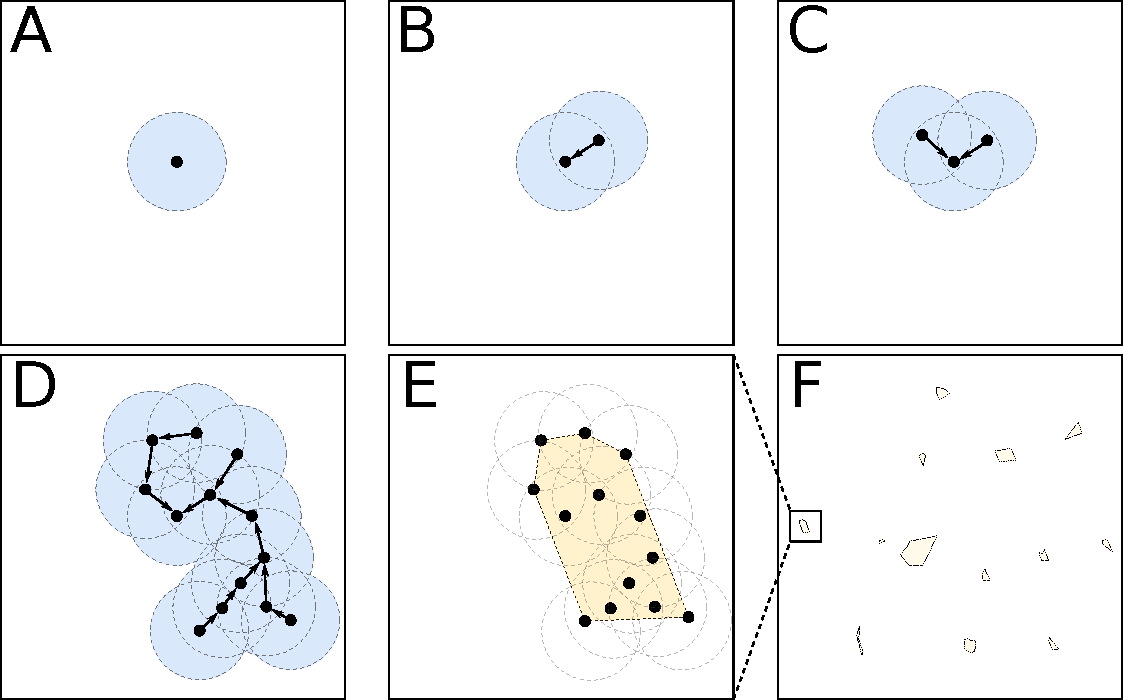
\includegraphics[width=.98\linewidth]{img/init_fp.pdf}
	\caption[Étapes successives de l'initialisation des foyers paysans agrégés (petites villes et villages).]{Étapes successives de l'initialisation des foyers paysans agrégés (petites villes et villages).\\
	(\textit{A) On génère un foyer paysan qui est positionné de manière aléatoire ;\\
	(B) on génère un nouveau foyer paysan dans un rayon donné du premier ;\\
	(C) et (D) on continue à générer de nouveaux foyers paysans dans le rayon de n'importe lequel des foyers existants ;\\
	(E) la géométrie d'un agrégat correspond à l'enveloppe convexe des foyers paysans ;\\
	(F) en fin d'initialisation, les étapes A à E ont été répétées pour le nombre d'agrégats initiaux défini, et l'ensemble des agrégats sont donc dispersés dans l'espace actif (voir \cref{fig:espace-simfeodal}) du modèle.}}
	\label{fig:init-fp}
\end{figure}


\paragraph{Seigneurs.}
Parmi les seigneurs, on distingue deux types : les grands seigneurs, sans représentation spatiale, et les petits seigneurs, localisés dans l'espace du modèle, toujours au sein d'un agrégat.
L'initialisation spatiale des seigneurs ne concerne donc que les petits seigneurs, dont on estime empiriquement le nombre initial à une vingtaine**.

À l'initialisation de \simfeodal{}, on répartit ces seigneurs dans l'espace du modèle, d'une manière aléatoire contrainte dans la mesure où il s'agit de les positionner dans un des agrégats créés à l'étape précédente.
Pour chaque seigneur, un premier tirage aléatoire est donc effectué pour déterminer dans quel agrégat il est situé, et un deuxième tirage pour le placer au sein de la délimitation de cet agrégat.
Plusieurs seigneurs peuvent ainsi être situés dans le même agrégat, et certains agrégats peuvent ne contenir aucun seigneur.

%Le mécanisme de création des premiers seigneurs est tout aussi simple et aléatoire : on répartit, de manière toujours aléatoire, un nombre donné de grands seigneurs.\\
%On localise aussi, selon un aléa contraint, un ensemble\footref{ftn:nombre-parametrable} de petits seigneurs au sein des agrégats existants, lesquels ont été délimités selon le mécanisme standard (voir \cref{meca-agregats}).
%Les petits seigneurs générés se voient directement associés à une zone de prélèvement de type \og foncier\fg{}, de rayon et de taux de prélèvement aléatoires bornés : dès l'initialisation, les premières zones de prélèvement sont donc créées.

\subsection{Paramètres d'initialisation}

Dans la partie précédente, on a plusieurs fois indiqué que certaines des valeurs numériques de l'initialisation étaient paramétrables, c'est-à-dire qu'on peut les faire varier afin de générer des structures spatiales initiales différentes à l'échelle macrogéographique.
Cela participe à la recherche de caractérisation de l'espace support initial de \simfeodal{}, où il n'y a pas d'\og \textit{input}\fg{} en tant que tel, mais un ensemble de paramètres qui influent sur les différents sous-modèles (voir \cref{sec:inputs}).
Pour l'initialisation, les paramètres sur lesquels on peut jouer pour tester différents scénarios sont précisés dans le \cref{tab:params-initiaux}.

\begin{table}[H]
	\centering
	{\renewcommand{\arraystretch}{1.2}%
	\begin{tabular}{|M{2.15cm}|M{4cm}|m{5.25cm}|m{1.25cm}|}
		\hline
		\textbf{Sous-mécanisme} & \textbf{Paramètre} & \textbf{Intitulé} & \textbf{Valeur} \\ \hline
		\makecell{Création\\du\\ \og monde\fg{} \\ du modèle} & Dimension & taille\_cote\_monde & 80 km \\ \hline
		\multirow{7}{*}{\makecell{Génération\\des\\Foyers\\Paysans\\(FP)}} & Nombre total de FP & init\_nb\_total\_fp & 4000 \\ \cline{2-4} 
		& Nombre de petites villes & init\_nb\_agglos & 8 \\ \cline{2-4} 
		& Nombre de FP par petite ville & init\_nb\_fp\_agglo & 30 \\ \cline{2-4} 
		& Nombre de villages & init\_nb\_villages & 20 \\ \cline{2-4} 
		& Nombre de FP par village & init\_nb\_fp\_village & 10 \\ \cline{2-4} 
		& Distance d'agrégation des FP & distance\_detection\_agregat & 100 m \\ \cline{2-4} 
		& \makecell{Taux de FP \\ \og dépendants\fg{}\\(ie. non mobiles)} & proba\_fp\_dependant & 20\% \\ \hline
		\multirow{2}{*}{\makecell{Génération\\des\\Églises}} & Nombre total d'églises & init\_nb\_eglises & 150 \\ \cline{2-4} 
		& (dont) Nombre d'églises paroissiales & init\_nb\_eglises\_paroissiales & 50 \\ \hline
		\multirow{3}{*}{\makecell{Génération\\des\\Seigneurs}} & Nombre de Grands Seigneurs & init\_nb\_gs & 2 \\ \cline{2-4} 
		& \makecell{Puissance relative\\des Grands Seigneurs\footnotemark} & \makecell{puissance\_grand\_seigneur$1$ \\ \textelp{} \\ puissance\_grand\_seigneur$N$} & 50\% \\ \cline{2-4} 
		& Nombre de Petits Seigneurs & init\_nb\_ps & 18 \\ \hline
	\end{tabular}}
	\caption{Paramètres permettant de contrôler l'initialisation du monde de SimFeodal.}
\label{tab:params-initiaux}
\end{table}
\begin{center}
	\hl{\large Problème de numérotation interrompue des notes de bas de page !}
\end{center}
\footnotetext{
	Ces paramètres sont plus spécifiques que les autres présentés ici et n'ont pas été introduits avant.
	Ils conditionnent la part des loyers que les grands seigneurs collectent.
	Voir la \cref{fig:prelevement-fonciers}, dans la \cref{sssec:collecte-droits}, p.~\pageref{fig:prelevement-fonciers}.
}

\let\orisectionmark\sectionmark
\renewcommand\sectionmark[1]{}%
\section[Données en entrée -- \textit{Input data}]{Données en entrée -- \large{\textit{Input data}} \label{sec:inputs}}
\orisectionmark{Données en entrée}
\let\sectionmark\orisectionmark

L'initialisation de \simfeodal{} constitue un sous-mécanisme à part entière, entièrement endogène au modèle.
À ce titre, on ne peut dire que des données en entrée (\textit{inputs}) contrôlent l'état initial du modèle, tel que c'est la norme dans des modèles spatiaux classiques (cf. \cref{sec:initialisation}).
Pour autant, on peut voir une forme d'\textit{inputs} dans les nombreux paramètres mobilisés pour l'initialisation et dans ceux, plus nombreux encore, qui influencent l'ensemble des mécanismes.

Par exemple, pour mettre en place des comportements exogènes permettant de faire varier le modèle à différentes dates précises, on peut classiquement faire appel à des données de sortie d'un autre modèle, ou à un fichier de configuration.
Dans \simfeodal{}, cette logique est bien présente, mais est gérée directement au sein du modèle, sans faire appel à des données externes.
Certains paramètres prennent ainsi la forme de tableaux d'associations (aussi appelés dictionnaires, ou \og \texttt{map}\fg{} en informatique), qui mettent en correspondance des valeurs de paramètres à des dates précises (voir \cref{lst:maps-gama}).
\medskip

{\footnotesize
	\begin{lstlisting}[caption={
	Deux exemples de \texttt{map} dans Gama.
	\textit{À partir de 800, les églises doivent se situer entre 5 et 25~km, puis entre 3 et 10~km de 960 à 1060, et entre 1.5 et 5~km après cette date.}}, captionpos=b, label={lst:maps-gama}]
map<int,int> dist_min_eglise <- [800::5000, 960::3000, 1060::1500];
map<int,int> dist_max_eglise <- [800::25000, 960::10000, 1060::5000]; 
	\end{lstlisting}
}

%Comme indiqué, il n'y a pas véritablement d'\textit{inputs} dans \simfeodal{} : tout est paramètre, et dès lors dynamique.
%En même temps, le modèle comporte de très nombreux paramètres : entre une quarantaine et une soixantaine selon les définitions possibles de ce qu'est un paramètre, voir \hl{chapitre 4}.\\
%On peut donc voir dans la multiplicité des paramètres une proximité avec la notion de données en entrée, qui ne s'expriment toutefois pas sous la forme traditionnelle.

%Pour respecter le formalisme ODD que suit ce chapitre, on peut au final considérer que \simfeodal{} est un modèle qui ne repose sur aucune donnée en entrée.
%Conceptuellement, le rôle joué par les paramètres du modèle s'en approche toutefois assez fortement.
%Le \hl{chapitre 4} permet d'éclairer cette description en entrant plus en détail dans la définition et la nomenclature des paramètres.

Quand bien même ce n'est pas le sens traditionnel d'\textit{inputs}, la multiplicité des paramètres et leur forte diversité remplit le même rôle (voir \cref{chap:chap3}, \cref{sssec:types-parametres}).
Il s'agit de contrôler précisément l'initialisation du modèle, mais aussi des éléments et événements indispensables, sur le plan empirique, qui ne doivent pas émerger des interactions du modèle, mais au contraire, les conditionner.


\let\orisectionmark\sectionmark
\renewcommand\sectionmark[1]{}%
\section[Mécanismes spécifiques -- \textit{Submodels}]{Mécanismes spécifiques -- \large{\textit{Submodels}}\label{sec:meca-specifiques}}
\orisectionmark{Mécanismes spécifiques}
\let\sectionmark\orisectionmark


\subsection{Introduction}

Cette partie du chapitre est plus technique et vise à présenter précisément différents mécanismes de \simfeodal{} évoqués dans la partie relative au fonctionnement général du modèle (\cref{sec:fonctionnement-general}).
Nous avons fait le choix de présenter les mécanismes sous la forme, discursive et schématique, la plus courte et compréhensible possible, quand bien même cette forme n'est qu'un \og modèle\fg{} de la réalité de l'implémentation : les formalismes, souvent graphiques, empruntés ici ne peuvent entièrement correspondre à l'implémentation effective en lignes de code.
De la même manière qu'une traduction d'une langue à une autre ne peut transcrire toutes les nuances originelles (\textit{traduttore}, \textit{traditore}), le passage d'une suite d'instruction algorithmiques à un formalisme plus accessible ne peut se faire sans quelques approximations.
Ces écarts entre présentation discursive des mécanismes et implémentation effective sont discutés dans l'\cref{enc:polarite-implementation}.
Dans un objectif de lisibilité, on a en effet choisi de ne pas entreprendre une description détaillée et exhaustive de tous les détails d'implémentation.
Il nous semble que ces éléments présentent un intérêt fondamental en termes de reproductibilité, mais qu'une description très précise présenterait aussi un caractère redondant avec le code-source du modèle.
Celui-ci est disponible publiquement\footnote{
	À l'adresse \href{https://github.com/SimFeodal/SimFeodal}{https://github.com/SimFeodal/SimFeodal}, voir l'\hyperlink{avant-propos}{avant-propos}
} et est partie intégrante de ce travail de thèse.
Sa reproduction à l'écrit, dans ces pages, même sous forme d'annexe, nous semble assez peu appropriée.
Cela n'enlève en rien, en revanche, de notre point de vue, à l'importance de sa consultation pour une compréhension plus fine du modèle.

%Notons aussi que la présentation des mécanismes n'est pas nécessairement exacte, c'est-à-dire une description fidèle de la manière dont les mécanismes sont implémentés informatiquement sous forme de codes-sources.

On remarquera enfin que nous avons préféré présenter ces mécanismes spécifiques dans un ordre différent de celui de l'ordonnancement dans le modèle (cf. \cref{fig:ordonnancement}), en les regroupant plutôt suivant les types d'agents concernés.
On présentera d'abord les mécanismes \og globaux\fg{}, c'est-à-dire relevant de la détection des agrégats, des pôles et des logiques de promotion et de création des paroisses ; puis les mécanismes relatifs aux foyers paysans ; et enfin ceux impliquant l'action des seigneurs.

\bigskip 
\begin{encadre}{Écarts entre présentation et implémentation}{polarite-implementation}
		\renewcommand{\thempfootnote}{\alph{mpfootnote}}
La présentation des mécanismes d'un modèle ne suit pas toujours la manière dont ces mécanismes sont implémentés dans le code-source d'un modèle.
C'est naturellement vrai entre deux \og domaines\fg{} d'un modèle -- si l'on reprend la triade des domaines conceptuels, empirique et informatique de \textcite[\ppno~3, fig. 2]{sargent2009verification} --
%\hl{(Lena : à reproduire quelque part dans la thèse)}
, au vu des écarts qu'il peut y avoir par exemple entre le modèle conceptuel et le modèle implémenté.
Toutefois, cela peut aussi se produire au sein d'un même domaine, par exemple ici pour le domaine du modèle informatique (\og computerized model\fg{} chez Sargent), notamment dans la phase de l'implémentation.
La présentation discursive d'un modèle suit ses règles propres, par exemple la nécessité de suivre une progression linéaire.
L'implémentation informatique, au contraire, ne suit pas forcément les mêmes règles, et tend même à requérir des logiques très différentes au nom d'une \og optimisation\fg{} du code-source, propre à chaque langage informatique.
Dans cet encadré, nous souhaitons mettre en avant trois types de processus où la présentation discursive et l'implémentation effective sont différentes tout en menant à des aboutissements équivalents.
Cette typologie ne vise pas l'exhaustivité, mais s'articule autour d'exemples rencontrés dans la présentation du modèle \simfeodal{}.

\paragraph{Point de vue de l'implémentation.} Quand un tirage aléatoire probabiliste est appliqué sur un grand nombre d'entités, son espérance théorique tend vers une fréquence empirique, en vertu de la loi des grands nombres.
En simulation à base d'agents, cela signifie que choisir une proportion de 10\% d'une large population (ce que l'on pourrait qualifier de \og probabilité de groupe\fg{}) est quasi-équivalent à doter chacun des individus d'une probabilité de $0.1$ d'être choisis (ce qui correspond à une \og probabilité individuelle\fg{}).
Cette équivalence est fortement mobilisée dans \simfeodal{}, le \og point de vue\fg{} -- probabilité individuelle ou de groupe -- changeant parfois à plusieurs reprises dans un même mécanisme, selon la praticité ou la performance (informatique) de l'une ou de l'autre.
Dans la description du modèle, l'objectif, pour des raisons de clarté, est d'avoir la vision la plus \og agent-centrée\fg{} possible.
On présentera préférentiellement les mécanismes comme faisant appel à des probabilités individuelles, quand bien même l'implémentation effective se fonde sur une approche proportionnelle, mobilisant des probabilités de groupe.

\paragraph{Factorisation.} Un autre écart entre description et implémentation tient à l'ordre d'exécution des sous-mécanismes par un ensemble d'agents.
En mathématiques, $k\times (x+y)$ est égal, selon les règles de factorisation, à $k{\cdot}x + k{\cdot}y$.
Dans un système multi-agents, la logique est la même.
On considère ainsi que même si l'ordre d'appel des agents diffère lors de l'implémentation d'un sous-mécanisme donné, ce qui peut faire varier le résultat, les sous-mécanismes décrits sont équivalents (plutôt qu'égaux).
Les programmes \ref{lst:facto1} et \ref{lst:facto2} sont ainsi considérés comme équivalents en dépit de la différence dans leur ordre d'appel.
Le premier programme demande à tous les agents, chacun leur tour, d'effectuer les mécanismes A et B successivement.
Le second est légèrement différent en ce qu'il demande d'abord à tous les agents d'effectuer A, et une fois que A est réalisé pour chacun, d'effectuer B.\bigskip

\noindent\begin{minipage}[b]{.45\textwidth}
	\begin{lstlisting}[caption={Factorisé},frame=tlrb, captionpos=b, label = {lst:facto1}]
ask agents [
 do A;
 do B;
]
	\end{lstlisting}
\end{minipage}\hfill
\begin{minipage}[b]{.45\textwidth}
	\begin{lstlisting}[caption={Développé},frame=tlrb, captionpos=b, label = {lst:facto2}]
ask agents [
 do A; ]
ask agents [
 do B; ]
	\end{lstlisting}
\end{minipage}

En termes d'efficacité du code, l'alternance entre ces deux approches permet de résoudre certaines difficultés d'implémentation.
On peut ainsi factoriser les calculs légers et au contraire développer les calculs plus lourds, par exemple pour faciliter l'enregistrement de variables intermédiaires liées à l'itération. 
En revanche, dans le cadre d'une description discursive, il sera souvent plus aisé de présenter les sous-processus de manière développée plutôt que factorisée pour bien différencier les étapes successives.

\paragraph{Optimisation.} Les deux types de processus précédents peuvent être combinés, pour répondre à des questions d'optimisation informatique, par exemple pour permettre au modèle de fonctionner plus rapidement en fonction des spécificités des langages informatiques choisis.
Dans Gama, par exemple, il est plus lent, informatiquement, de calculer la distance depuis 1000 agents à 10 agents, que l'inverse, quand bien même les résultats sont strictement identiques.
Le calcul de la satisfaction de protection des foyers paysans en offre un exemple.
Il requiert de mesurer la distance de chaque agent concerné au château le plus proche.
Il est ainsi bien plus rapide de calculer cette mesure depuis les châteaux, puis de sélectionner la distance minimale pour chaque couple (foyer paysan; château).
On voit donc bien dans cet exemple que l'implémentation se fait dans un sens opposé à celui du discours, sans que cela ait la moindre conséquence sur le plan conceptuel.
\end{encadre}

\subsection{Mécanismes globaux}

Dans cette sous-partie, nous présentons le détail des mécanismes \og globaux\fg{}, c'est-à-dire des mécanismes qui sont exécutés au niveau global du modèle, et non au niveau des agents (voir le paragraphe dédié dans l'introduction de \cref{sec:fonctionnement-general}).

Même s'ils ne résultent pas de comportements des agents, ces mécanismes sont indispensables au modèle en ce qu'ils dessinent le contexte spatial dans lequel les agents-foyers paysans évolueront et seront en interaction.
À ce titre, ces mécanismes ont une influence très importante sur le déroulé du modèle, et ont donc été changés, adaptés et améliorés de nombreuses fois.
Cette forte évolutivité se transcrit par des mécanismes parfois très spécifiques, dont les étapes peuvent être nombreuses, de même que les cas particuliers au regard de telles ou telles conditions vis-à-vis des agents.

\subsubsection{Identification des agrégats \label{sssec:agregats}}

La \cref{fig:detection-agregats} présente les étapes successives de détection des agrégats.
À chaque pas de temps, on repart d'une situation \og neutre\fg{}, c'est-à-dire que tous les foyers paysans sont considérés comme dispersés (\textbf{A}).
On exécute un algorithme de classification basé sur la distance\footnote{
	L'opérateur Gama \textsf{simple\_clustering\_by\_distance}, proche conceptuellement de l'algorithme DBSCAN.
} : les \textit{clusters} constitués d'au moins 5 foyers paysans espacés de moins de 100~m sont considérés comme des agrégats (\textbf{B}).
On fixe alors la géométrie des agrégats, qui prend la forme de l'enveloppe convexe des foyers paysans qui les composent (\textbf{C}).
Les foyers paysans inclus dans la surface d'un agrégat y sont ajoutés (\textbf{D}).
	
\begin{figure}[H]
	\centering
	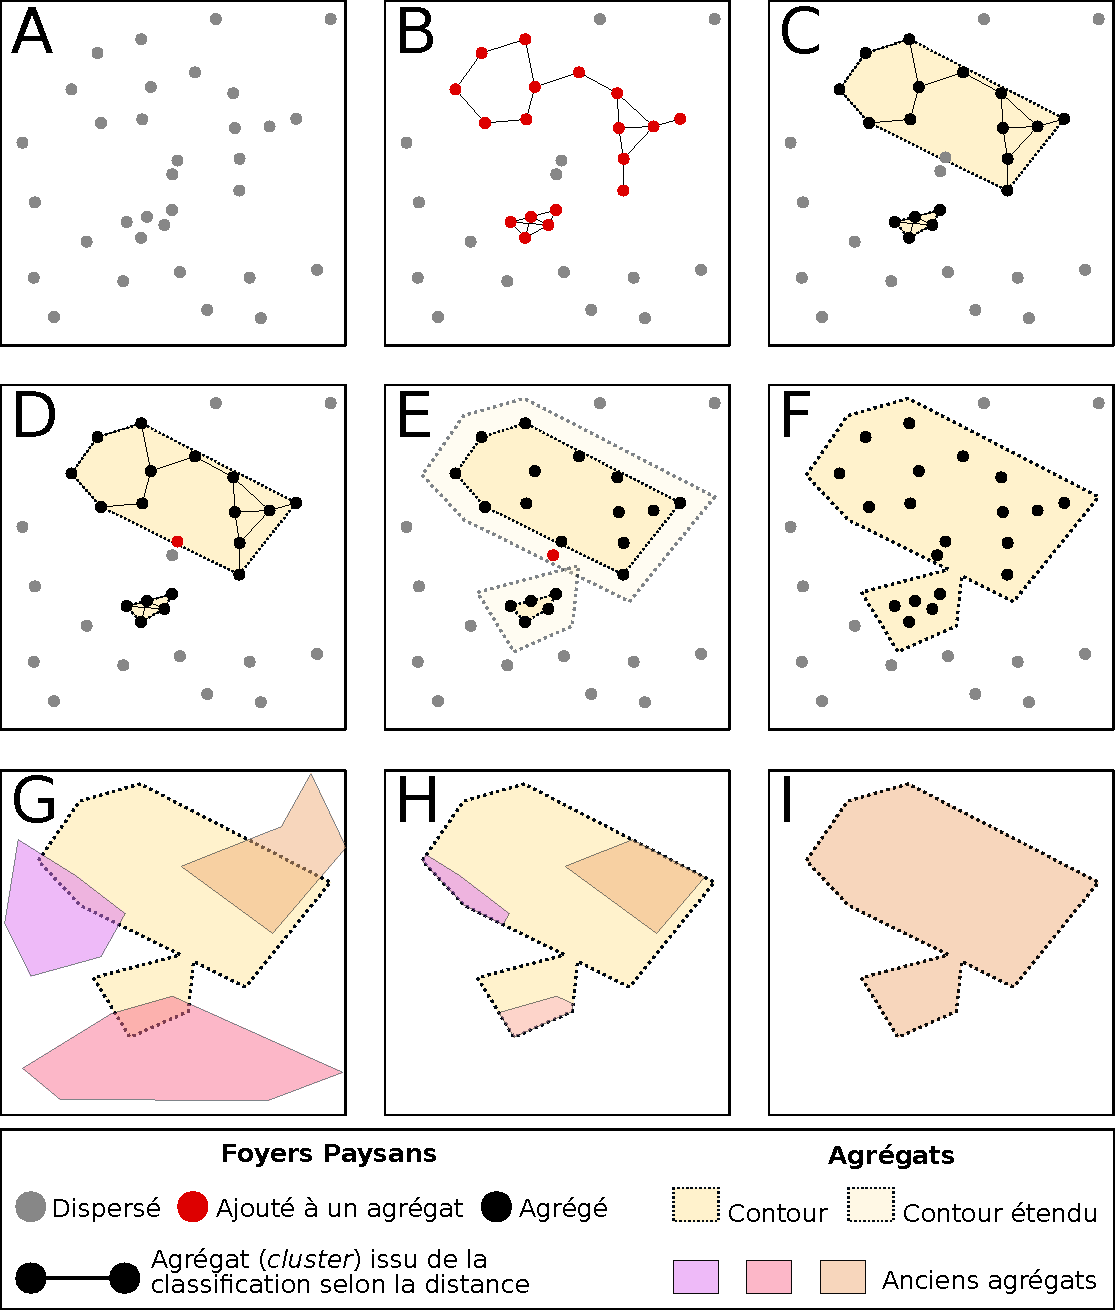
\includegraphics[width=.75\linewidth]{img/detection_agregats.pdf}
	\caption{Détection des agrégats et identification de leur \og héritage\fg{}.}
	\label{fig:detection-agregats}
\end{figure}

On crée ensuite des \textit{buffers} de 100~m autour des agrégats et on y rattache à nouveau les foyers paysans inclus dans la surface (\textbf{E}).
Dernière étape dans la détection des agrégats, pour ne pas multiplier les agrégats proches les uns des autres, on procède à une étape de fusion en réalisant l'union géométrique des agrégats qui s'intersectent (\textbf{F}).\\
Les trois dernières étapes concernent la transmission des propriétés des agrégats à travers les pas de temps et, en particulier, de la présence ou non d'une communauté en leur sein.
On isole les agrégats du pas de temps précédent qui intersectent les nouveaux agrégats (\textbf{G}).
On procède ensuite à une intersection entre les géométries de ces anciens agrégats et le nouvel agrégat (\textbf{H}).
Le nouvel agrégat hérite alors des propriétés de l'ancien agrégat dont la superficie d'intersection est la plus importante (l'agrégat orange dans l'étape \textbf{I}).
	
\subsubsection{Identification des pôles \label{sssec:poles}}

Les pôles sont des agents composés d'attracteurs de trois types (cf. \cref{fig:constitution-poles-paroisses}-\textbf{A}) : les châteaux (petits et gros), les églises (dotées de droits paroissiaux) et les agrégats (comportant une communauté).
Notons que les églises simples ou les agrégats ne comportant pas de communauté villageoise ne sont pas considérés comme des attracteurs.
Les pôles et leur délimitation spatiale revêtent une importance particulière lors de la migration des foyers paysans : ils attirent d'autant plus que leur attractivité est importante et, le cas échéant, les foyers paysans migrants s'installent à l'intérieur de leur délimitation.
La \cref{fig:detection-poles} illustre la méthode de définition spatiale des pôles, ainsi que des exemples de calcul de leurs attractivités.

\begin{figure}[H]
	\centering
	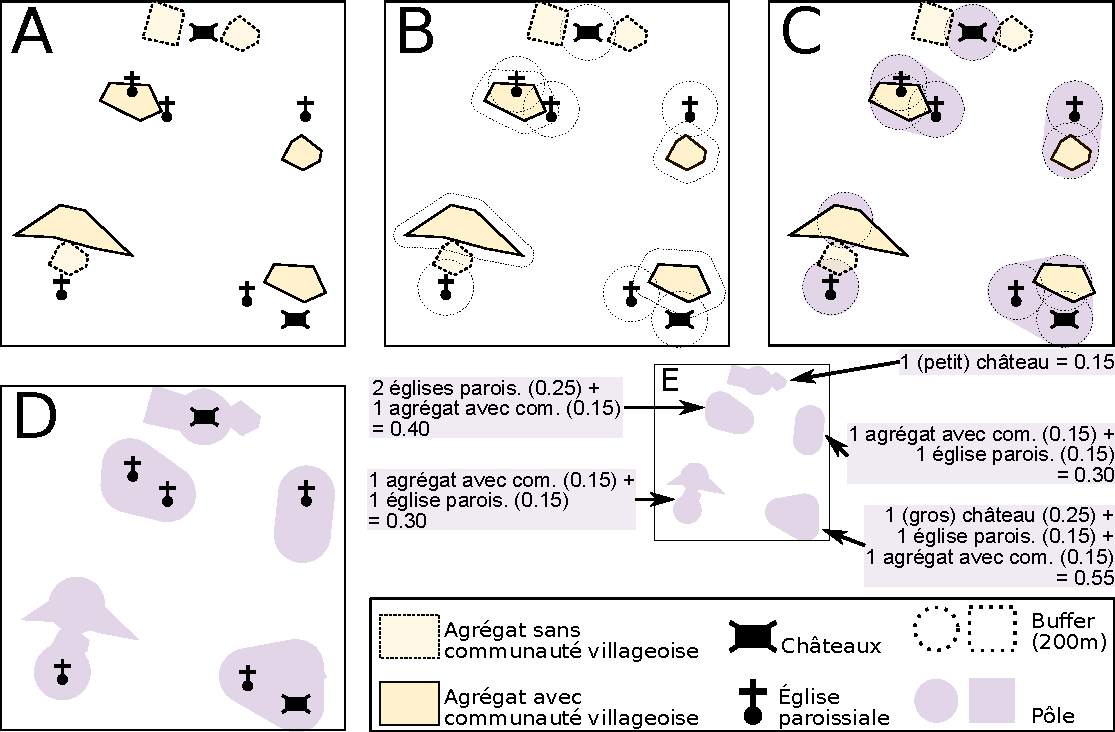
\includegraphics[width=\linewidth]{img/detection_poles.pdf}
	\caption{Les étapes du mécanisme de détection et de calcul d'attractivité des pôles.}
	\label{fig:detection-poles}
\end{figure}

À chaque pas de temps, on repart d'une situation \og neutre\fg{}, c'est-à-dire que l'on recalcule systématiquement les pôles sans repartir des pas de temps précédents (\textbf{A}).
On commence par identifier les attracteurs situés à moins de 200~m les uns des autres (\textbf{B}) pour identifier les pôles qui peuvent être constitués de plusieurs attracteurs proches, ou d'un unique attracteur.
L'enveloppe spatiale des pôles est définie comme un \textit{buffer} de 200~m autour de l'enveloppe convexe formée par le centroïde des attracteurs qui les composent (\textbf{C}).
Il s'agit par conséquent d'un cercle de rayon de 200~m pour les pôles mono-attracteurs, et d'un polygone pour les pôles composites.
Pour que les agrégats proches d'un pôle soient bien identifiés comme en faisant partie, on fusionne (union géométrique) l'enveloppe spatiale des pôles avec les contours de l'ensemble des agrégats (comportant ou non une communauté paysanne) intersectés.
Cela permet à des pôles peu éloignés de fusionner à leur tour (\textbf{D}).
On peut enfin calculer leur attractivité à partir des seuils définis dans le \cref{tab:attraction-poles} (\textbf{E}).

\begin{table}[H]
	\centering
	{\renewcommand{\arraystretch}{1.1}%
	\begin{tabular}{|l|l|l|}\hline
		\textbf{Attracteur} & \textbf{Détail} & \textbf{Attractivité} \\ \hline
		\multirow{2}{*}{Châteaux} & Petit & 0.15 \\
		& Gros & 0.25 \\ \hline
		\multirow{4}{*}{Église paroissiale} & 1 & 0.15 \\
		& 2 & 0.25 \\
		& 3 & 0.5 \\
		& 4+ & 0.6 \\ \hline
		\multicolumn{2}{|l|}{Agrégat (doté d'une communauté)} & 0.15 \\ \hline
	\end{tabular}}
\caption[Attractivité conférée aux pôles par leurs attracteurs.]{Attractivité ($\in [0,1]$) conférée aux pôles par leurs attracteurs.}
\label{tab:attraction-poles}
\end{table}


	
\subsubsection{Création et promotion d'églises paroissiales \label{sssec:paroisses}}

Dans les zones peu denses, c'est-à-dire hors agrégat, de nouvelles églises paroissiales peuvent apparaître soit par promotion, soit par création.
Dans le premier cas, c'est une église existante, qui n'a pas de droits paroissiaux, qui sera promue et deviendra église paroissiale.
Dans le second cas, c'est-à-dire quand il n'y a pas d'église non paroissiale qui satisfasse aux critères spatiaux, une nouvelle église est créée et directement dotée des droits paroissiaux.

Dans les zones faiblement peuplées, c'est-à-dire là où peu d'agrégats sont présents, la population des foyers paysans doit aussi être desservie par des églises paroissiales.
Quand une paroisse comporte plus de 20 foyers paysans insatisfaits sur le plan religieux, elle cherche à se subdiviser en créant une nouvelle église paroissiale.
Celle-ci peut être une église non dotée de droits paroissiaux qui se verrait promu, ou donner lieu à la création d'une nouvelle église, directement dotée de droits paroissiaux.
Les paragraphes suivants résument les différentes manières de renforcer le maillage paroissial, autour de l'exemple de quatre paroisses \og insatisfaisantes\fg{} (\textbf{A}, \textbf{B}, \textbf{C} et \textbf{D}, voir \cref{fig:promotion-paroisses-base}).

\begin{figure}[H]
	\centering
	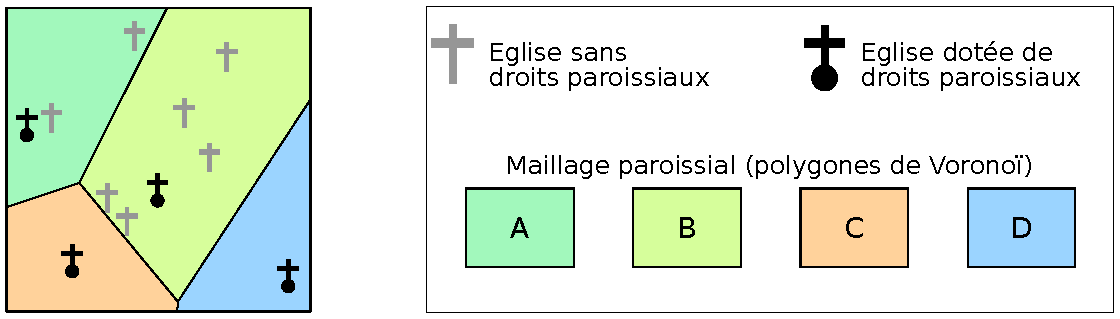
\includegraphics[width=1\linewidth]{img/promo_creation_paroisses_base.pdf}
	\caption{Quatre exemples de paroisses insatisfaisantes.}
	\label{fig:promotion-paroisses-base}
\end{figure}


\subparagraph{Promotion d'églises paroissiales en présence d'églises non paroissiales.}
Les deux paroisses \textbf{A} et \textbf{B} de cet exemple contiennent chacune des églises non paroissiales dont l'une pourra être promue en église paroissiale (\cref{fig:promotion-paroisses-1}).

\begin{figure}[H]
	\centering
	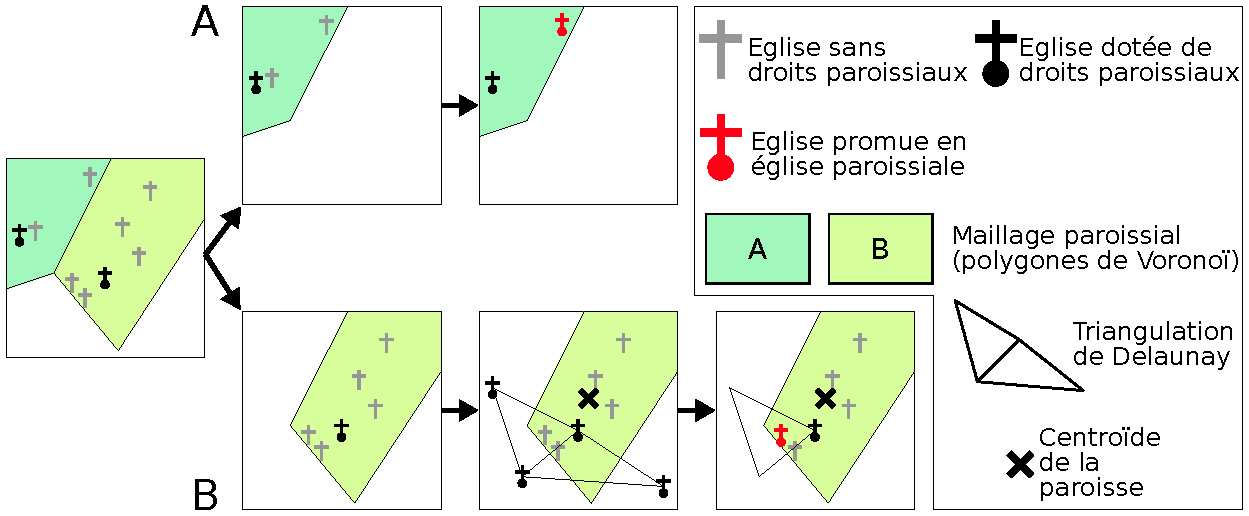
\includegraphics[width=1\linewidth]{img/promo_creation_paroisses_promo1.pdf}
	\caption{Promotion d'églises paroissiales avec églises non paroissiales.}
	\label{fig:promotion-paroisses-1}
\end{figure}

\begin{itemize}
	\item S'il y a au plus 3 églises non paroissiales disponibles dans la maille de la paroisse (\textbf{A}), on en sélectionne une aléatoirement et on la promeut en église paroissiale.
	
	\item S'il y a plus de trois églises non paroissiales disponibles (\textbf{B}), on réalise une triangulation de Delaunay autour de toutes les églises paroissiales (les églises \textbf{A}, \textbf{B}, \textbf{C} et \textbf{D}, visibles dans la \cref{fig:promotion-paroisses-base}).\\
	Puis, on sélectionne le triangle résultant qui est le plus proche du centroïde de la paroisse.\\
	Enfin, on promeut en église paroissiale l'église la plus proche du centre de ce triangle et appartenant à la paroisse.	
\end{itemize}


\subparagraph{Paroisses sans églises non paroissiales.}

Les deux paroisses situées en bas (\textbf{C} et \textbf{D}) de l'exemple ne contiennent pas d'églises non paroissiales (\cref{fig:promotion-paroisses-2}).

\begin{figure}[H]
	\centering
	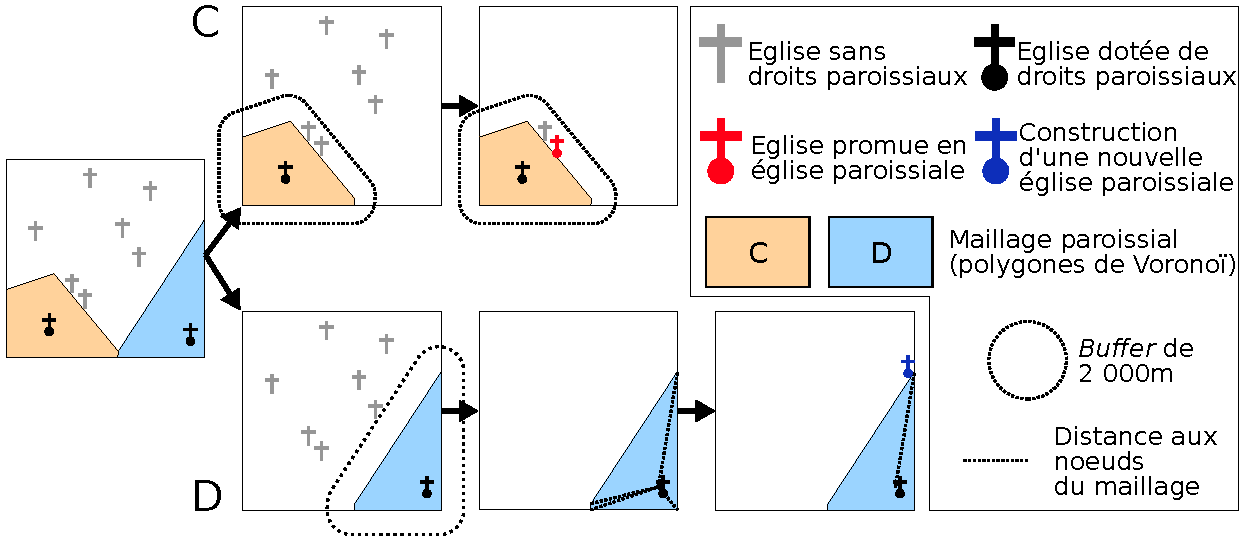
\includegraphics[width=1\linewidth]{img/promo_creation_paroisses_promo2.pdf}
	\caption{Promotion et création d'églises paroissiales dans des paroisses n'ayant initialement pas d'églises sans droits paroissiaux.}
	\label{fig:promotion-paroisses-2}
\end{figure}

Dans ce cas de figure, on cherche les églises non paroissiales situées dans un rayon de 2000 m autour de la paroisse.
\begin{itemize}
	\item Si des églises non paroissiales sont présentes dans ce \textit{buffer} (\textbf{C}), on en sélectionne une de manière aléatoire et on lui attribue des droits paroissiaux.
	
	\item S'il n'y a aucune église non paroissiale dans ce \textit{buffer} de 2 000 m (\textbf{D}), on bâti une nouvelle église.\\
	Celle-ci sera localisée sur le sommet du polygone paroissial le plus éloigné de l'église paroissiale existante.
\end{itemize}

%	
%	\begin{figure}[H]
%		\centering
%		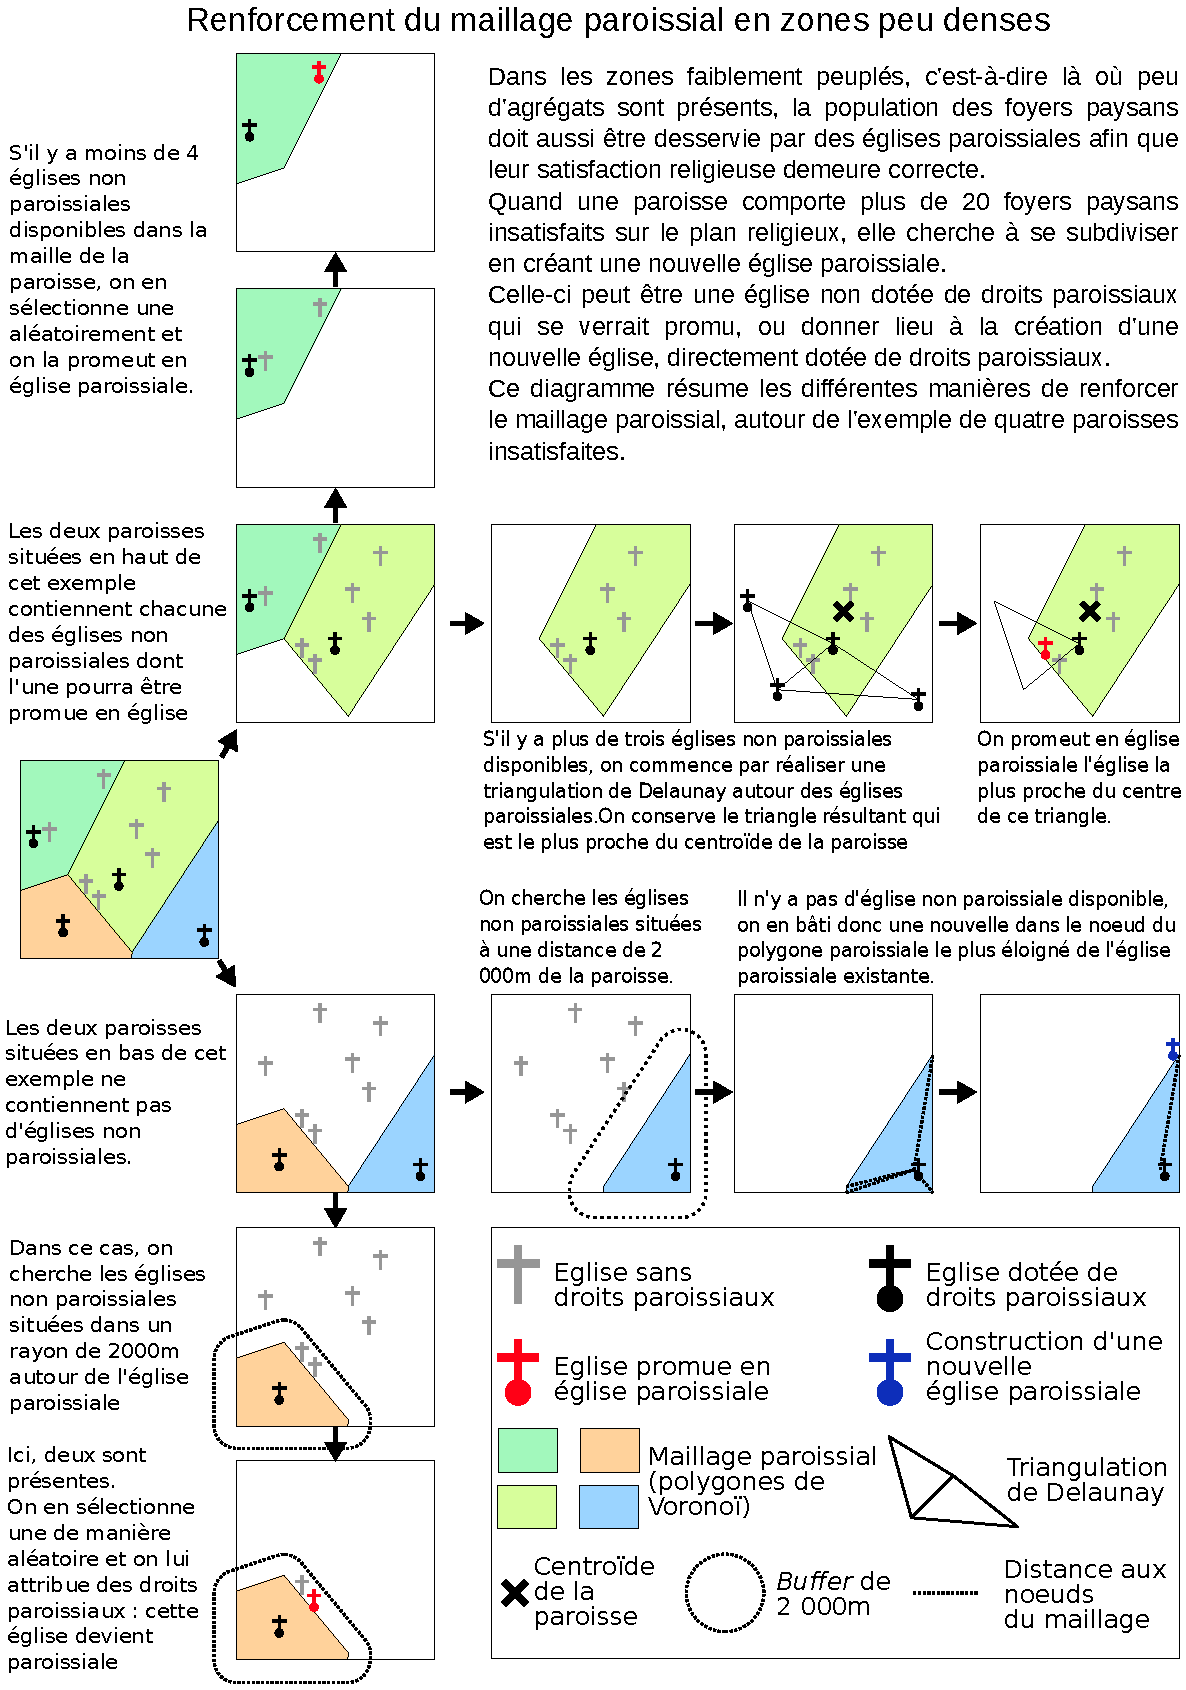
\includegraphics[width=1\linewidth]{img/constru-promo_paroisses_rurales.pdf}
%		\caption{Construction et promotion de paroisses en zone peu dense.}
%		\label{fig:promotion-paroisses}
%	\end{figure}
	
\subsection{Foyers paysans}

	\subsubsection{Satisfaction et modèles gravitaires \label{sssec:satisfaction}}
	
Les satisfactions religieuses et de protection des foyers paysans suivent une logique proche du modèle gravitaire : plus les foyers sont éloignés des \og attracteurs\fg{} (les châteaux pour la satisfaction \og protection\fg{} ; les églises paroissiales pour la satisfaction religieuse), moins ils sont satisfaits.
Cette logique simple est légèrement contrainte par l'introduction de seuils :
	 en dessous d'une certaine distance (\textit{distance\_min}), le foyer paysan est entièrement satisfait (satisfaction = 1), et au delà d'une distance (\textit{distance\_max}), sa satisfaction est nulle (satisfaction = 0).
Entre ces deux seuils, minimal et maximal, la satisfaction suit une logique gravitaire simple, associée à une décroissance linéaire.
L'équation \ref{eq:satisfaction-distance} permet de formaliser ce type de calcul, et la \cref{fig:satisfaction-distance} illustre cette relation.

\begin{figure}[H]
	\centering
	\begin{equation}\label{eq:satisfaction-distance}
	\begin{gathered}
	satis\_dist = min \left \lbrack max \left \lbrack \frac{(distance_{max} - distance\_attracteur)}{(distance_{max} -distance_{min})}; 0 \right \rbrack ; 1 \right \rbrack
	\end{gathered}
	\end{equation}
	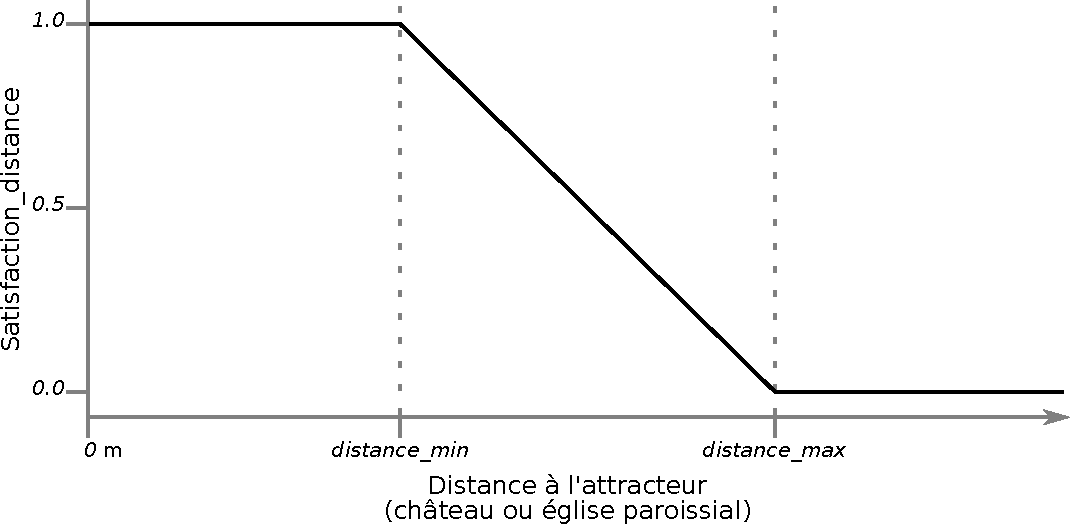
\includegraphics[width=.8\linewidth]{img/satisfaction_distance.pdf}
	\caption{Variation de la satisfaction en fonction de la distance à l'attracteur le plus proche.}
	\label{fig:satisfaction-distance}
\end{figure}

\paragraph{Satisfaction religieuse.}
		
Le calcul de la satisfaction religieuse s'inscrit rigoureusement dans cette logique.
On peut le formuler ainsi :
		\begin{equation*}
		s_{religieuse} = min \left \lbrack max \left \lbrack \frac{(distance_{max} - distance\_eglise)}{(distance_{max} -distance_{min})}; 0 \right \rbrack ; 1 \right \rbrack
		\end{equation*}
avec des seuils de distance ($distance\_max$ et $distance\_min$) qui évoluent au cours du temps :
\begin{itemize}
	\item avant 960 : $distance_{min}$ = 5 km et $distance_{max}$ = 25 km
	\item de 960 à 1060 : $distance_{min}$ = 3 km et $distance_{max}$ = 10 km
	\item après 1060 : $distance_{min}$ = 1,5 km et $distance_{max}$ = 5 km
\end{itemize}
Ces seuils, tenant compte de notamment de l'augmentation de la fréquence obligatoire de visite des églises paroissiales, ont été déterminés par les archéologues et historiens participant au projet.

	
\paragraph{Satisfaction \og protection\fg{}.}	

La satisfaction \og protection\fg{} mobilise une logique semblable, c'est-à-dire qu'elle est fonction de la distance au château le plus proche.
Cette distance est ici pondérée par un paramètre ($besoin\_protection$) qui permet de prendre en compte la sensibilité des foyers paysans au climat de violence, lequel tend à augmenter pendant la période.

\begin{equation*}
s_{protection} = (s_{distance\_chateau})^{(besoin\_protection)}
\end{equation*}
avec
\begin{equation*}
\begin{gathered}
s_{distance\_chateau} = min \left \lbrack
max \left \lbrack \frac{(dist_{max} - distance\_chateau)}{(dist_{max} -distance_{min})}; 0.01 \right \rbrack ; 1 \right \rbrack
\end{gathered}
\end{equation*}
($dist_{min}$ = 1,5 km et $dist_{max}$ = 5 km )
et un paramètre de sensibilité évoluant au cours du temps ($besoin\_protection$)  :
\begin{itemize}
	\item avant 960 : $besoin\_protection = 0 $
	\item de 960 à 1020 : $besoin\_protection = 0.2 ; 0.4 ; 0.6 ; 0.8$ (augmente de $0.2$ à chaque pas de temps)
	\item après 1020 : $besoin\_protection = 1$
\end{itemize}

\paragraph{Satisfaction matérielle.}

La satisfaction matérielle ne prend aucune distance en compte : elle s'appuie sur le montant des taxes dont le foyer paysan doit s'acquitter ($redevance\_acquittees$).
Ce montant est pondéré par un paramètre technique représentant un niveau \og acceptable\fg{} de taxation ($coef\_redevances$, qui vaut $15$ ici, c'est-à-dire qu'un foyer paysan s'acquittant de 15 droits ou plus aura une satisfaction matérielle de 0).

L'appartenance du foyer paysan à une communauté permet aussi de pondérer l'influence des redevances acquittées : plus le paramètre $puissance\_communaute$ est important, moins la satisfaction matérielle du foyer paysan sera affectée par les droits dont il s'acquitte.
La valeur de ce paramètre est par ailleurs évolutive : elle augmente au fur et à mesure de la période modélisée\footnote{
	$puissance\_communaute$ vaut $0.2$ jusqu'en 1060, puis augmente de $0.2$ à chaque pas de temps pour atteindre $1$ en 1140 et rester à ce niveau.
}.
Cela permet d'intégrer le rôle croissant, connu empiriquement, des communautés paysannes.


\begin{equation*}
\begin{gathered}
s_{materielle} = (s_{redevance})^{(1-puissance\_communaute)}
\end{gathered}
\end{equation*}
avec 
\begin{equation*}
\begin{gathered}
s_{redevance} = max \left[ \left( 1- \frac{redevances\_acquittees}{coef\_redevances} \right) ; 0 \right]
\end{gathered}
\end{equation*}

\paragraph{Satisfaction générale.}

La satisfaction générale est mesurée à partir du minimum de ces satisfactions individuelles.
Ce choix traduit l'hypothèse que ces satisfactions ne s'équilibrent pas.
Une \og satisfaction protection\fg{} forte ne compensera pas une forte insatisfaction religieuse par exemple.
En revanche l'appartenance du foyer paysan à une communauté intervient directement dans la satisfaction générale, cette appartenance tendant à l'augmenter.
L'appartenance à une communauté paysanne intervient ainsi à deux reprises dans le calcul de la satisfaction, une fois dans le calcul de la satisfaction matérielle et ensuite dans le calcul de la satisfaction générale.
Ce choix permet de tenir compte du poids que prennent ces structures sociales et institutionnelles au cours de la période modélisée.


Le calcul de la satisfaction s'exprime ainsi :
\begin{equation*}
\begin{split}
satisfaction =~& 0.75 \times \left[ min \left( s_{materielle} ; s_ {religieuse}; s_{protection} \right) \right] + \\
& 0.25 \times [appartenance\_communaute]
\end{split}
\end{equation*}
avec $ \{satisfaction ; s_{materielle} ; s_ {religieuse} ; s_{protection}\} \in [0,1]$ et $[appartenance\_communaute] \in \{0;1\} $


	\subsubsection{Migration des foyers paysans \label{sssec:migration}}

La migration des foyers paysans est sans doute le mécanisme le plus complexe et qui a été le plus modifié depuis la conception de \simfeodal{}.
La règle d'ensemble est pourtant extrêmement simple : un foyer paysan a une probabilité de migrer qui est proportionnelle à son insatisfaction. 
Autrement dit, $P \left( migration \right) = \left( 1 - satisfaction \right)$.
Cette règle simple a été progressivement complexifiée afin d'augmenter la rationalité et l'ancrage empirique des choix de localisation.
Cette complexification du mécanisme est inhérente au choix de modélisation, KIDS, dans lequel \simfeodal{} s'inscrit (cf. \cref{subsec:explorer-confronter}), et où l'on cherche à suivre autant que possible les connaissances empiriques, quitte à complexifier plus que de nécessaire (par rapport au niveau de détail des autres mécanismes) certaines règles.

Une première complexification a abouti à la distinction de migrations \og locales\fg{} et de migrations \og lointaines\fg{} (voir \cref{fig:migrations-locales-lointaines}).

\begin{figure}[H]
\centering
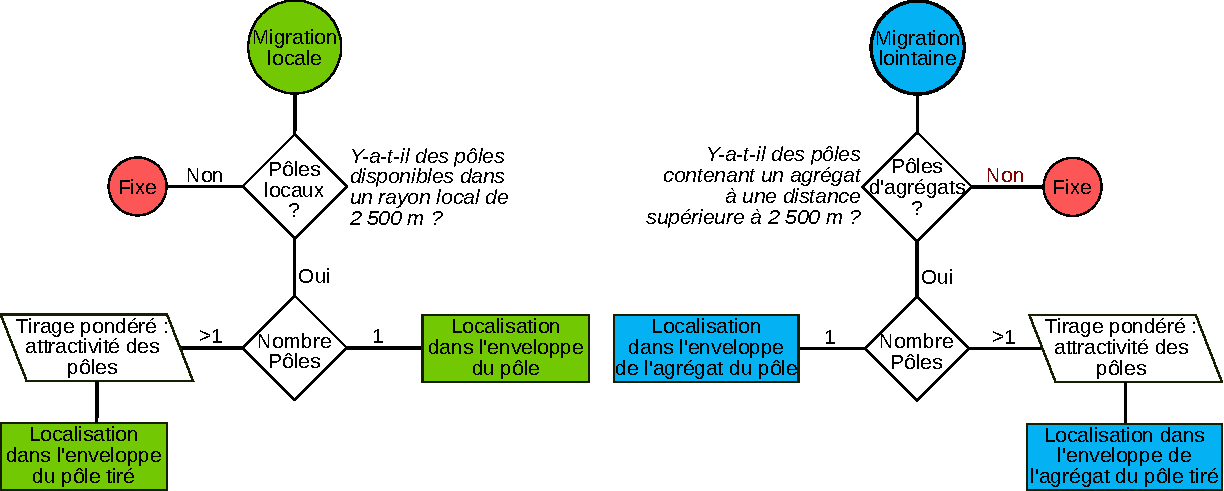
\includegraphics[width=1\linewidth]{img/migration_locale-lointaine.pdf}
\caption{Migrations locales et lointaines.}
\label{fig:migrations-locales-lointaines}
\end{figure}
Pour aboutir à cette différence entre migration locale et migration lointaine, la règle repose sur le fait que les foyers paysans privilégient les migrations locales.
Quand celles-ci ne sont pas possibles, ils ont une probabilité (plus faible) d'effectuer une migration lointaine.
Afin de prendre en compte les connaissances empiriques sur la migration des foyers paysans de cette époque, nous avons introduit une légère différence de comportement entre les foyers paysans déjà agrégés et ceux qui sont dispersés lors de l'exécution du mécanisme de migration (\cref{fig:choix-migration}).
On a ainsi considéré qu'un foyer paysan déjà agrégé cherchait un agrégat potentiellement plus attractif, afin de voir sa satisfaction augmenter, tandis qu'un foyer paysan dispersé cherchait avant tout à rejoindre un agrégat, en faisant preuve de moins d'exigence dans son choix.

\begin{figure}[H]
	\centering
	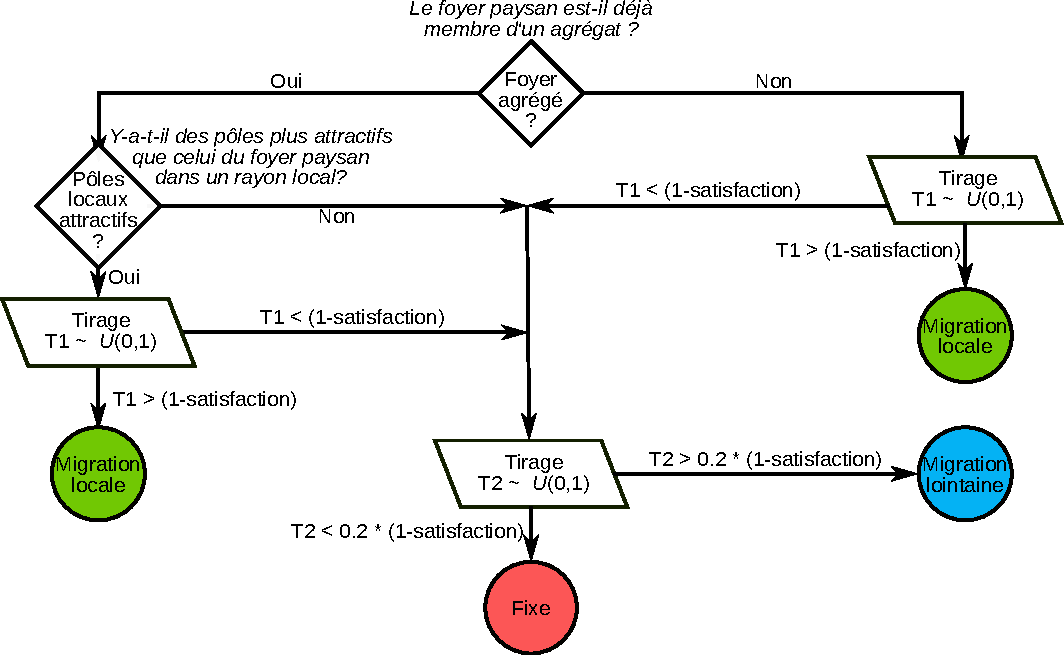
\includegraphics[width=0.9\linewidth]{img/choix_migration.pdf}
	\caption{Décision de migration.}
	\label{fig:choix-migration}
\end{figure}

Une dernière distinction a été opérée entre les foyers paysans classiques, libres de leurs choix migratoires, et les foyers paysans \og dépendants\fg{}.
Ces derniers représentent les foyers qui n'ont pas le droit de quitter le domaine de leur seigneur (les serfs entre autres).
Ceux-là ne peuvent effectuer que des migrations locales, et on considère qu'ils seront amenés à migrer plus facilement, les migrations locales ayant un \og coût\fg{} moindre pour le foyer paysan.

Cette nouvelle distinction, comme les précédentes, s'inscrit encore dans le processus de modélisation KIDS : pour les thématiciens, la distinction entre foyers paysans \og mobiles\fg{} et foyers paysans \og dépendants\fg{} est importante empiriquement, et devait être prise en compte dans le modèle.
Le mécanisme spécifique de migration des foyers paysans dépendants est présenté dans la \cref{fig:choix-migration-dependants}.


\begin{figure}[H]
	\centering
	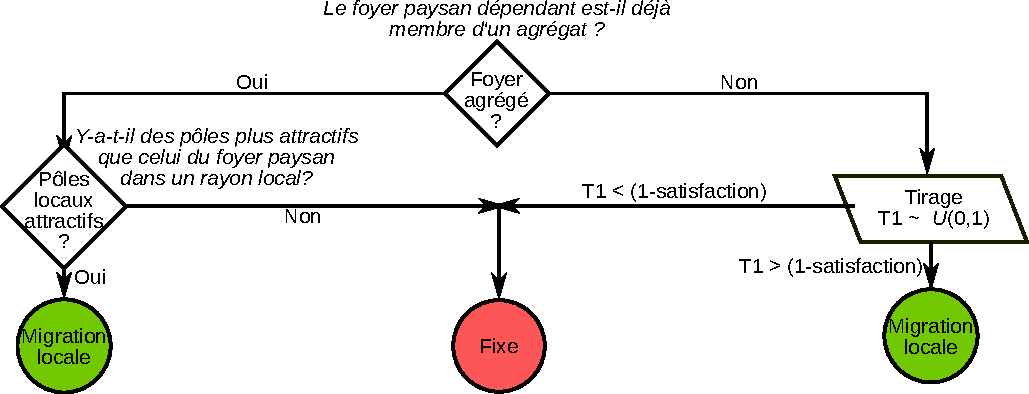
\includegraphics[width=0.9\linewidth]{img/choix_migration_dependants.pdf}
	\caption{Décision de migration des foyers paysans dépendants.}
	\label{fig:choix-migration-dependants}
\end{figure}
 

\subsection{Seigneurs}
	\subsubsection{Prélèvement des droits \label{sssec:collecte-droits}}
\setcounter{footnote}{\value{savefootnote}}
Les seigneurs, petits et grands, collectent les taxes dont doivent s'acquitter les foyers paysans (droits de haute justice et autres droits) majoritairement (exception faite des droits fonciers pour les grands seigneurs, voir \cref{fig:prelevement-fonciers}) par l'intermédiaire des zones de prélèvement.
Ces zones sont caractérisées par un propriétaire (le seigneur qui les possède), éventuellement un gardien (le seigneur à qui la zone a été \og donnée\fg{}, voir \cref{meca-dons}), une localisation\footnote{
	Pour les petits seigneurs, il s'agit de leur propre localisation
}, un rayon\footnote{
	Ce rayon est tiré aléatoirement suivant une distribution uniforme, \\$rayon\_zp \sim \mathcal{U}\left[ rayon\_min\_zp\_ps , rayon\_max\_zp\_ps \right]$, avec $rayon\_min\_zp\_ps$ et $rayon\_max\_zp\_ps$ des paramètres qui valent respectivement 1 000 et 5 000 m.\\
	N.B : zp = zone de prélèvement et ps = petit seigneur
} et un taux de prélèvement\footnote{
	idem : $taux\_prelevement\_zp \sim \mathcal{U}\left[ min\_taux\_prelevement\_zp\_ps , max\_taux\_prelevement\_zp\_ps \right]$ avec $min\_taux\_prelevement\_zp\_ps$ et $max\_taux\_prelevement\_zp\_ps$ valant 5\% et 25\%.
}.
%À noter que les zones de prélèvement liées à des châteaux suivent une règle légèrement différente, que nous n'aborderons pas ici\footnote{Se référer au code-source du modèle, dans la fonction \textsf{construction\_chateaux}}.

Les prélèvements rapportent de la \og puissance\fg{} aux seigneurs, différenciés selon les types de droits (\cref{tab:puissance-droits}).

\begin{table}[H]
	\centering
	{\renewcommand{\arraystretch}{1.1}%
		\begin{tabular}{|l|l|l|}\hline
			\textbf{Type de droit} & \textbf{Fonction du seigneur} & \textbf{\makecell{Puissance acquise\\par foyer paysan}} \\ \hline
			\multirow{2}{*}{Haute Justice} & Propriétaire ou Gardien & 2 \\
			& Souverain (zone donnée) & 2.5 \\ \hline
			\multirow{2}{*}{Droits fonciers} & Propriétaire ou Gardien & 1 \\
			& Souverain (zone donnée) & 1.25 \\ \hline
			\multirow{2}{*}{Autres droits} & Propriétaire ou Gardien & 0.25 \\
			& Souverain (zone donnée) & 0.35 \\ \hline	
	\end{tabular}}
\caption{Gain de puissance par foyer paysan prélevé.}
\label{tab:puissance-droits}
\end{table}


\paragraph{Foncier.}

Quelques petits seigneurs (tous ceux créés dès l'initialisation ainsi que $\approx 10\%$ de ceux créés pendant le déroulement de la simulation) possèdent des droits fonciers.
À ce titre, ils peuvent collecter ces droits au sein d'une zone de prélèvement qu'ils créent lors de leur apparition.
Le mécanisme de collecte des droits fonciers est illustré par la \cref{fig:prelevement-fonciers}.
\begin{figure}[H]
	\centering
	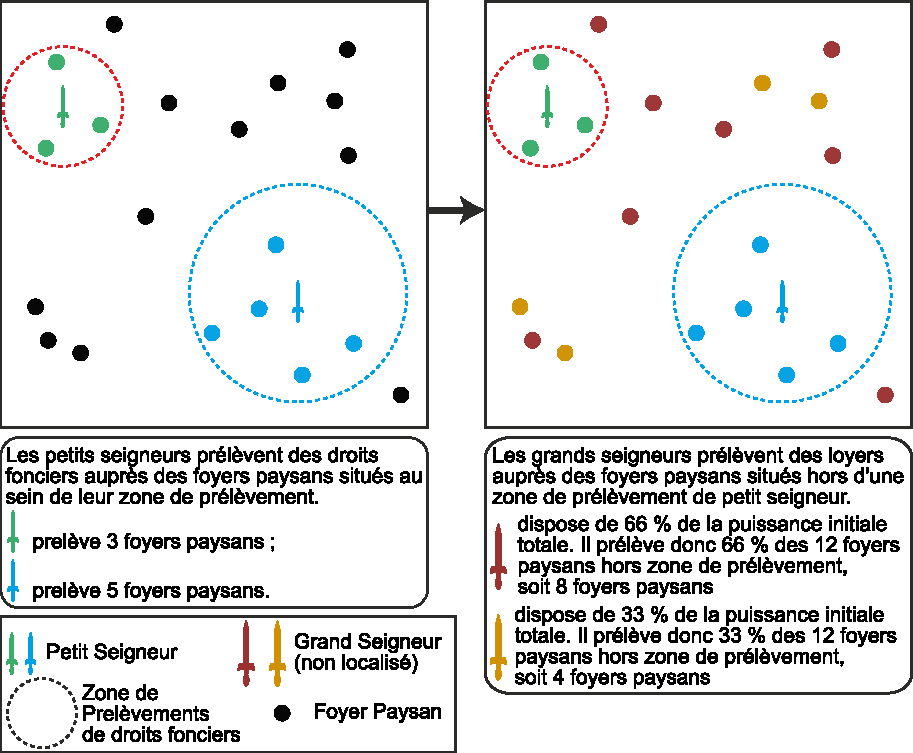
\includegraphics[width=0.8\linewidth]{img/prelevements_foncier.pdf}
	\caption{Prélèvement des droits fonciers par les petits et grands seigneurs.}
	\label{fig:prelevement-fonciers}
\end{figure}

\paragraph{Haute justice et autres droits.}

Les autres droits suivent un mécanisme plus générique : les seigneurs propriétaires collectent des droits auprès d'une partie des foyers paysans inclus dans la surface de la zone de prélèvement.
Cette partie correspond aux \og taux de prélèvement\fg{} décrit plus haut. La \cref{fig:prelevement-droits} récapitule les différentes modalités de collecte de droits via les zones de prélèvement.

La partie (b) de la figure (prélèvements multiples) illustre le cas où un même seigneur possède plusieurs zones de prélèvement concentriques, et où les taux de prélèvement partiels (20\% et 25\% dans cet exemple) s'appliquent donc en partie aux mêmes foyers paysans.
Du point de vue du foyer paysan, cela montre qu'avec ces deux zones, un même foyer paysan situé dans la zone de prélèvement de plus faible rayon peut se voir prélevé 0, 1 ou 2 droits, affectant sa satisfaction matérielle en conséquence.

\begin{figure}[H]
	\centering
	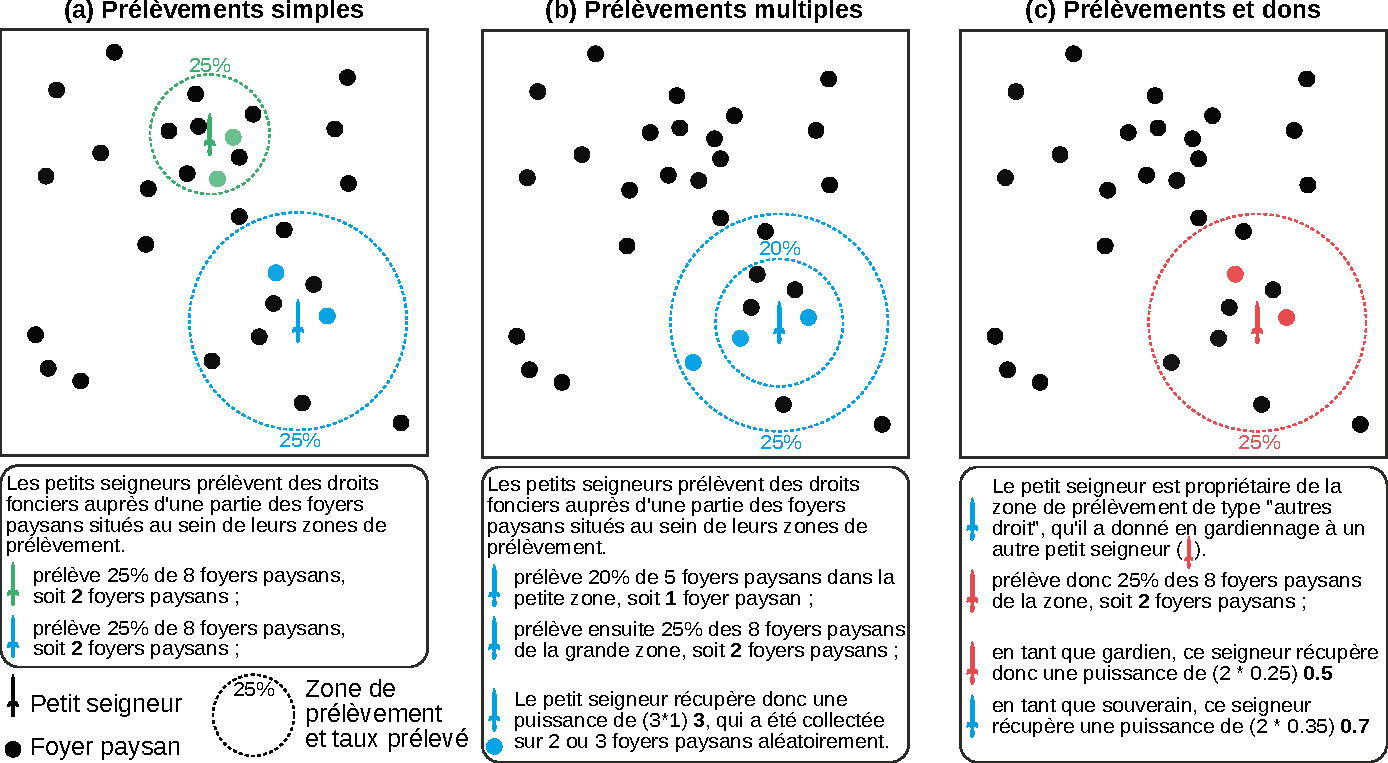
\includegraphics[width=\linewidth]{img/prelevements_droits.pdf}
	\caption{Mécanisme général de prélèvement des droits par les seigneurs.}
	\label{fig:prelevement-droits}
\end{figure}

Les droits de haute justice sont prélevés exactement comme les autres droits, à la seule différence qu'ils correspondent nécessairement à des taux de prélèvement de 100\%.

\subsubsection{Construction de châteaux \label{sssec:constru-chateaux}}


À partir de 940, les seigneurs ont la possibilité de créer des châteaux, dans un espace limité par la présence d'autres châteaux : on considère ainsi, au regard des connaissances empiriques, que deux châteaux ne peuvent être espacés de moins de 3 000 mètres.
Le mécanisme de construction des châteaux est commun aux grands et aux petits seigneurs, mais certains paramètres varient selon le type du seigneur considéré :
\begin{itemize}
	\item Un grand seigneur peut construire jusqu'à $2$ châteaux par tour (paramètre $nb\_max\_chateaux\_par\_tour\_gs$), alors qu'un petit seigneur peut en construire au maximum $1$ par pas de temps ($nb\_max\_chateaux\_par\_tour\_ps$).
	\item Pour un seigneur $i$, la probabilité de construire un château est formalisée ainsi :\\
	$$ P \left( construction \right) = \frac{puissance\_seigneur_{i}}{\sum{puissance\_seigneur_{1..n}}} \times ponderation\_proba\_chateau $$ avec $ponderation\_proba\_chateau$ valant $1.25$ pour les grands seigneurs et $7$ pour les petits (paramètres techniques).
	\item Les grands seigneurs peuvent construire des châteaux n'importe-où dans l'espace du modèle (en respectant toutefois les règles exposées plus bas), alors que les petits seigneurs ne peuvent le faire que dans un rayon de 5 000 m de leur localisation : s'il n'y a pas d'espace disponible dans ce rayon, le petit seigneur ne crée pas de château.
\end{itemize}

Les règles de localisation de château sont identiques et illustrées dans la \cref{fig:construction-chateaux}.

\begin{figure}[H]
	\centering
	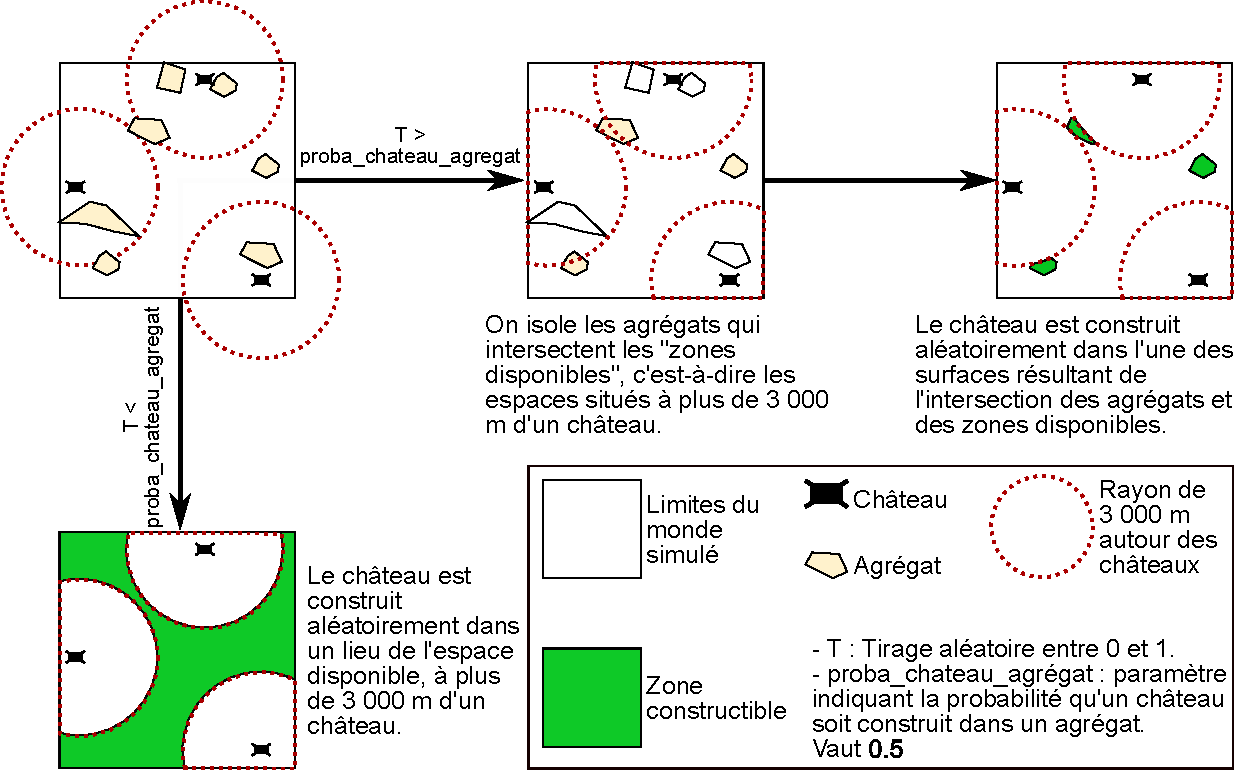
\includegraphics[width=\linewidth]{img/construction_chateaux.pdf}
	\caption{Mécanisme de localisation des châteaux construits.}
	\label{fig:construction-chateaux}
\end{figure}

\paragraph{Rayon des zones de prélèvement associées.}

La construction d'un château implique systématiquement la création de zones de prélèvements qui lui sont associées, c'est-à-dire qu'elles appartiennent au seigneur qui crée le château.
Si le château est donné en gardiennage, l'ensemble des zones de prélèvement qui lui sont associées seront aussi données en gardiennage au petit seigneur choisi.

Les zones de prélèvement créées concernent des droits fonciers et des autres droits.
Si le seigneur châtelain obtient les droits de haute justice, une zone de prélèvement de droits de haute justice sera automatiquement créée autour de chacun de ses châteaux.

Contrairement aux zones de prélèvement habituelles, celles qui sont associées à un château ont un taux de prélèvement de $100\%$.
Cette particularité est due à l'importance thématique des châteaux, qui remplissent un rôle de protection au prix d'un investissement important.
Cela implique dès lors que les prélèvements y sont plus élevés et systématiques que dans les zones plus classiques.
Dans \simfeodal{}, cela est modélisé sous la forme de ce taux de prélèvement supérieur à la norme et par à un rayon, lui aussi, supérieur.
Ce dernier est variable et dépend de la puissance relative du seigneur qui construit le château.
Plus précisément, le rayon varie entre un seuil minimal de 2 000 m ($rayon\_min\_zp\_chateau$) et un seuil maximal de 15 000 m ($rayon\_max\_zp\_chateau$).
Entre ces deux seuils, la valeur du rayon dépend d'une fonction linéaire correspondant au ratio entre la puissance du seigneur constructeur et les puissances maximales et minimales de l'ensemble des seigneurs, tel que formalisé dans l'équation \ref{eq:rayon-zp-chateau}. 

\begin{equation}\label{eq:rayon-zp-chateau}
\begin{aligned}
& rayon\_zp\_chateau = \\
& min \left[ max \left[ puissance\_relative; rayon\_min\_zp\_chateau \right] ; rayon\_max\_zp\_chateau \right]
\\
& \text{avec}
\\
& puissance\_relative_i = \frac{max(puissance_{0..n}) - puissance_i}{max(puissance_{0..n}) \times min(puissance_{0..n})}
\end{aligned}
\end{equation}

\section*{Conclusion}
\addcontentsline{toc}{section}{Conclusion}

Le protocole de description ODD, suivi tout au long de ce chapitre, présente l'avantage indéniable de forcer les modélisateurs à harmoniser les présentations de leur modèle.
Cette harmonisation est \og interne\fg{}, en ce que le protocole demande de suivre un niveau homogène de présentation des propriétés et règles d'un modèle.
Il est ainsi nécessaire de présenter ces règles de manière simplifiée dans un premier temps (\textit{Process overview}, \cref{sec:fonctionnement-general}) puis détaillée par la suite (\textit{Submodels}, \cref{sec:meca-specifiques}).
Mais l'harmonisation est aussi \og externe\fg{}, chaque section poussant à positionner son modèle vis-à-vis d'autres modèles de simulation à base d'agents de la littérature, par exemple dans la partie des \og concepts de modélisation\fg{} (\cref{sec:design-concepts}), où le rapport des agents à l'environnement spatial ne peut être appréhendée qu'en comparaison avec des modèles connus.

Le prix de cette généricité et de cette contextualisation est une certaine inadaptation à certains modèles.
La dernière partie de ce chapitre, consacrée à la présentation détaillée de certains mécanismes, montre ainsi à quel point le protocole de description ODD peut être difficile à mobiliser pour des modèles descriptifs et exploratoires comme \simfeodal{}.
%Cela complique la démarche d'explicitation de ces mécanismes : 
%en voulant en simplifier la présentation, on a vite fait d'en dénaturer le fonctionnement réel.
Cette difficulté de présentation du modèle dans le cadre d'ODD est renforcée par la forte hétérogénéité, en termes de complexité\footnote{
Le terme complexité est ici employé au sens algorithmique, et non au sens des systèmes complexes.
Une plus forte complexité désigne ici un mécanisme plus \og compliqué\fg{}, régit par un nombre de règles, d'étapes ou de conditions plus importantes qu'un autre.
}, des mécanismes de \simfeodal{}.
On en a déjà mentionné les raisons dans l'introduction :
	les niveaux de précision des connaissances des différents objets modélisés sont très variables et liés aux parcours et sujets de recherche individuels des thématiciens impliqués dans la construction du modèle.
Si l'on ajoute une \og longue durée\fg{} de conception et de développement du modèle, qui plus est caractérisée par des allers-retours entre des phases de simplification et des phases de complexification, on ne peut qu'obtenir un modèle difficile à homogénéiser.
Tous ces éléments sont toutefois caractéristiques de la nature -- et de la vocation -- exploratoire de \simfeodal{}, dont le développement comporte sans doute plus de résultats que l'utilisation d'un état \og final\fg{}.

En dépit de cette forte hétérogénéité dans les mécanismes, il nous semble en revanche important de pointer aussi la certaine généricité qui en caractérise les fondations.
Par exemple, le calcul des différentes composantes de la satisfaction générale est assez similaire, autour de logiques de seuils minimum et maximum entre lesquels la satisfaction suit une logique linéaire.
Cette logique prédominait initialement dans de nombreux autres mécanismes (probabilité de construction de châteaux, probabilité de créer de nouvelles églises paroissiales\ldots), de même qu'une certaine logique gravitaire dans le choix des destinations de migration des foyers paysans.

Les nombreuses versions successives du modèle ont entrainé des spécifications de ces mécanismes autrefois très génériques, spécifications qui peuvent en masquer une logique initiale qui demeure cependant bien présente et que nous avons parfois essayé de rappeler.
Par exemple, les mécanismes de migration des foyers paysans (\cref{sssec:migration}) sont très particuliers et semblent fortement variables d'un cas à l'autre (migrations locales ou lointaines, migrations des foyers paysans \og mobiles\fg{} ou \og dépendants\fg{}), alors que toutes ces particularités sont autant de variations complexes autour d'une logique commune et simple, dans laquelle la probabilité de migrer est directement proportionnelle à l'insatisfaction (ie. $1 - satisfaction$).

Au cours du temps, le modèle a donc été complexifié par ses auteurs.
Cette complexification, ou spécification, visait d'une part à détailler des comportements pour les rendre plus représentatifs des connaissances thématiques, et d'autre part à en ajuster le fonctionnement en fonction des résultats sur lesquels ils aboutissaient.
Ce double objectif a défini le processus de \og paramétrage\fg{} qui a été réalisé, et visait ainsi à \og améliorer\fg{} le modèle.

Cette \og amélioration\fg{} ne peut s'entendre qu'au regard des objectifs du modèle, c'est-à-dire du questionnement initial auquel il doit permettre de répondre.
Pour cela, il est nécessaire de définir des critères permettant de qualifier la capacité du modèle à répondre à ces questions ainsi que la qualité de ces réponses.
En somme, après avoir présenté le fonctionnement du modèle, il est indispensable de revenir sur les raisons de ce fonctionnement, et aussi de présenter les modalités de ce qui a guidé le paramétrage de \simfeodal{}, à savoir son évaluation.
